%  A simple AAU report template.
%  2015-05-08 v. 1.2.0
%  Copyright 2010-2015 by Jesper Kjær Nielsen <jkn@es.aau.dk>
%
%  This is free software: you can redistribute it and/or modify
%  it under the terms of the GNU General Public License as published by
%  the Free Software Foundation, either version 3 of the License, or
%  (at your option) any later version.
%
%  This is distributed in the hope that it will be useful,
%  but WITHOUT ANY WARRANTY; without even the implied warranty of
%  MERCHANTABILITY or FITNESS FOR A PARTICULAR PURPOSE.  See the
%  GNU General Public License for more details.
%
%  You can find the GNU General Public License at <http://www.gnu.org/licenses/>.
%
%  A simple AAU report template.
%  2015-05-08 v. 1.2.0
%  Copyright 2010-2015 by Jesper Kjær Nielsen <jkn@es.aau.dk>
%
%  This is free software: you can redistribute it and/or modify
%  it under the terms of the GNU General Public License as published by
%  the Free Software Foundation, either version 3 of the License, or
%  (at your option) any later version.
%
%  This is distributed in the hope that it will be useful,
%  but WITHOUT ANY WARRANTY; without even the implied warranty of
%  MERCHANTABILITY or FITNESS FOR A PARTICULAR PURPOSE.  See the
%  GNU General Public License for more details.
%
%  You can find the GNU General Public License at <http://www.gnu.org/licenses/>.
%
\documentclass[11pt,twoside,a4paper,openright]{report}
%%%%%%%%%%%%%%%%%%%%%%%%%%%%%%%%%%%%%%%%%%%%%%%%
% Language, Encoding and Fonts
% http://en.wikibooks.org/wiki/LaTeX/Internationalization
%%%%%%%%%%%%%%%%%%%%%%%%%%%%%%%%%%%%%%%%%%%%%%%%
% Select encoding of your inputs. Depends on
% your operating system and its default input
% encoding. Typically, you should use
%   Linux  : utf8 (most modern Linux distributions)
%            latin1 
%   Windows: ansinew
%            latin1 (works in most cases)
%   Mac    : applemac
% Notice that you can manually change the input
% encoding of your files by selecting "save as"
% an select the desired input encoding. 
\usepackage[utf8]{inputenc}
% Make latex understand and use the typographic
% rules of the language used in the document.
\usepackage[danish,english]{babel}
% Use the palatino font
\usepackage[sc]{mathpazo}
\linespread{1.05}         % Palatino needs more leading (space between lines)
% Choose the font encoding
\usepackage[T1]{fontenc}
%%%%%%%%%%%%%%%%%%%%%%%%%%%%%%%%%%%%%%%%%%%%%%%%
% Graphics and Tables
% http://en.wikibooks.org/wiki/LaTeX/Importing_Graphics
% http://en.wikibooks.org/wiki/LaTeX/Tables
% http://en.wikibooks.org/wiki/LaTeX/Colors
%%%%%%%%%%%%%%%%%%%%%%%%%%%%%%%%%%%%%%%%%%%%%%%%
% load a colour package
\usepackage{xcolor}
\definecolor{aaublue}{RGB}{33,26,82}% dark blue
% The standard graphics inclusion package
\usepackage{graphicx}
% Set up how figure and table captions are displayed
\usepackage{caption}
\captionsetup{%
  font=footnotesize,% set font size to footnotesize
  labelfont=bf % bold label (e.g., Figure 3.2) font
}
% Make the standard latex tables look so much better
\usepackage{array,booktabs}
% Enable the use of frames around, e.g., theorems
% The framed package is used in the example environment
\usepackage{framed}

%%%%%%%%%%%%%%%%%%%%%%%%%%%%%%%%%%%%%%%%%%%%%%%%
% Mathematics
% http://en.wikibooks.org/wiki/LaTeX/Mathematics
%%%%%%%%%%%%%%%%%%%%%%%%%%%%%%%%%%%%%%%%%%%%%%%%
% Defines new environments such as equation,
% align and split 
\usepackage{amsmath}
% Adds new math symbols
\usepackage{amssymb}
% Use theorems in your document
% The ntheorem package is also used for the example environment
% When using thmmarks, amsmath must be an option as well. Otherwise \eqref doesn't work anymore.
\usepackage[framed,amsmath,thmmarks]{ntheorem}

%%%%%%%%%%%%%%%%%%%%%%%%%%%%%%%%%%%%%%%%%%%%%%%%
% Page Layout
% http://en.wikibooks.org/wiki/LaTeX/Page_Layout
%%%%%%%%%%%%%%%%%%%%%%%%%%%%%%%%%%%%%%%%%%%%%%%%
% Change margins, papersize, etc of the document
\usepackage[
  inner=28mm,% left margin on an odd page
  outer=41mm,% right margin on an odd page
  ]{geometry}
% Modify how \chapter, \section, etc. look
% The titlesec package is very configureable
\usepackage{titlesec}
\titleformat{\chapter}[display]{\normalfont\huge\bfseries}{\chaptertitlename\ \thechapter}{20pt}{\Huge}
\titleformat*{\section}{\normalfont\Large\bfseries}
\titleformat*{\subsection}{\normalfont\large\bfseries}
\titleformat*{\subsubsection}{\normalfont\normalsize\bfseries}
%\titleformat*{\paragraph}{\normalfont\normalsize\bfseries}
%\titleformat*{\subparagraph}{\normalfont\normalsize\bfseries}

% Clear empty pages between chapters
\let\origdoublepage\cleardoublepage
\newcommand{\clearemptydoublepage}{%
  \clearpage
  {\pagestyle{empty}\origdoublepage}%
}
\let\cleardoublepage\clearemptydoublepage

% Change the headers and footers
\usepackage{fancyhdr}
\pagestyle{fancy}
\fancyhf{} %delete everything
\renewcommand{\headrulewidth}{0pt} %remove the horizontal line in the header
\fancyhead[RE]{\small\nouppercase\leftmark} %even page - chapter title
\fancyhead[LO]{\small\nouppercase\rightmark} %uneven page - section title
\fancyhead[LE,RO]{\thepage} %page number on all pages
% Do not stretch the content of a page. Instead,
% insert white space at the bottom of the page
\raggedbottom
% Enable arithmetics with length. Useful when
% typesetting the layout.
\usepackage{calc}

%%%%%%%%%%%%%%%%%%%%%%%%%%%%%%%%%%%%%%%%%%%%%%%%
% Bibliography
% http://en.wikibooks.org/wiki/LaTeX/Bibliography_Management
%%%%%%%%%%%%%%%%%%%%%%%%%%%%%%%%%%%%%%%%%%%%%%%%
\usepackage[backend=bibtex,
  bibencoding=utf8
  ]{biblatex}
\addbibresource{bib/mybib}

%%%%%%%%%%%%%%%%%%%%%%%%%%%%%%%%%%%%%%%%%%%%%%%%
% Misc
%%%%%%%%%%%%%%%%%%%%%%%%%%%%%%%%%%%%%%%%%%%%%%%%
% Add bibliography and index to the table of
% contents
\usepackage[nottoc]{tocbibind}
% Add the command \pageref{LastPage} which refers to the
% page number of the last page
\usepackage{lastpage}
% Add todo notes in the margin of the document
\usepackage[
%  disable, %turn off todonotes
  colorinlistoftodos, %enable a coloured square in the list of todos
  textwidth=\marginparwidth, %set the width of the todonotes
  textsize=scriptsize, %size of the text in the todonotes
  ]{todonotes}

%%%%%%%%%%%%%%%%%%%%%%%%%%%%%%%%%%%%%%%%%%%%%%%%
% Hyperlinks
% http://en.wikibooks.org/wiki/LaTeX/Hyperlinks
%%%%%%%%%%%%%%%%%%%%%%%%%%%%%%%%%%%%%%%%%%%%%%%%
% Enable hyperlinks and insert info into the pdf
% file. Hypperref should be loaded as one of the 
% last packages
\usepackage{hyperref}
\hypersetup{%
	pdfpagelabels=true,%
	plainpages=false,%
	pdfauthor={Author(s)},%
	pdftitle={Title},%
	pdfsubject={Subject},%
	bookmarksnumbered=true,%
	colorlinks=false,%
	citecolor=black,%
	filecolor=black,%
	linkcolor=black,% you should probably change this to black before printing
	urlcolor=black,%
	pdfstartview=FitH%
}
% package inclusion and set up of the document

% see, e.g., http://en.wikibooks.org/wiki/LaTeX/Formatting#Hyphenation
% for more information on word hyphenation
\hyphenation{ex-am-ple hy-phen-a-tion short}
\hyphenation{long la-tex}% 
%  A simple AAU report template.
%  2015-05-08 v. 1.2.0
%  Copyright 2010-2015 by Jesper Kjær Nielsen <jkn@es.aau.dk>
%
%  This is free software: you can redistribute it and/or modify
%  it under the terms of the GNU General Public License as published by
%  the Free Software Foundation, either version 3 of the License, or
%  (at your option) any later version.
%
%  This is distributed in the hope that it will be useful,
%  but WITHOUT ANY WARRANTY; without even the implied warranty of
%  MERCHANTABILITY or FITNESS FOR A PARTICULAR PURPOSE.  See the
%  GNU General Public License for more details.
%
%  You can find the GNU General Public License at <http://www.gnu.org/licenses/>.
%
%
%
% see, e.g., http://en.wikibooks.org/wiki/LaTeX/Customizing_LaTeX#New_commands
% for more information on how to create macros

%%%%%%%%%%%%%%%%%%%%%%%%%%%%%%%%%%%%%%%%%%%%%%%%
% Macros for the titlepage
%%%%%%%%%%%%%%%%%%%%%%%%%%%%%%%%%%%%%%%%%%%%%%%%
%Creates the aau titlepage
\newcommand{\aautitlepage}[3]{%
  {
    %set up various length
    \ifx\titlepageleftcolumnwidth\undefined
      \newlength{\titlepageleftcolumnwidth}
      \newlength{\titlepagerightcolumnwidth}
    \fi
    \setlength{\titlepageleftcolumnwidth}{0.5\textwidth-\tabcolsep}
    \setlength{\titlepagerightcolumnwidth}{\textwidth-2\tabcolsep-\titlepageleftcolumnwidth}
    %create title page
    \thispagestyle{empty}
    \noindent%
    \begin{tabular}{@{}ll@{}}
      \parbox{\titlepageleftcolumnwidth}{
        \iflanguage{danish}{%
          
\includegraphics[width=\titlepageleftcolumnwidth]{figures/aau_logo_da}
        }{%
          
\includegraphics[width=\titlepageleftcolumnwidth]{figures/aau_logo_en}
        }
      } &
      \parbox{\titlepagerightcolumnwidth}{\raggedleft\sf\small
        #2
      }\bigskip\\
       #1 &
      \parbox[t]{\titlepagerightcolumnwidth}{%
      \textbf{Abstract:}\bigskip\par
        \fbox{\parbox{\titlepagerightcolumnwidth-2\fboxsep-2\fboxrule}{%
          #3
        }}
      }\\
    \end{tabular}
    \vfill
    \iflanguage{danish}{%
      \noindent{\footnotesize\emph{Rapportens indhold er frit tilgængeligt, men offentliggørelse (med kildeangivelse) må kun ske efter aftale med forfatterne.}}
    }{%
      \noindent{\footnotesize\emph{The content of this report is freely available, but publication (with reference) may only be pursued due to agreement with the author.}}
    }
    \clearpage
  }
}

%Create english project info
\newcommand{\englishprojectinfo}[8]{%
  \parbox[t]{\titlepageleftcolumnwidth}{
    \textbf{Title:}\\ #1\bigskip\par
    \textbf{Theme:}\\ #2\bigskip\par
    \textbf{Project Period:}\\ #3\bigskip\par
    \textbf{Project Group:}\\ #4\bigskip\par
    \textbf{Participant(s):}\\ #5\bigskip\par
    \textbf{Supervisor(s):}\\ #6\bigskip\par
    \textbf{Copies:} #7\bigskip\par
    \textbf{Page Numbers:} \pageref{LastPage}\bigskip\par
    \textbf{Date of Completion:}\\ #8
  }
}

%Create danish project info
\newcommand{\danishprojectinfo}[8]{%
  \parbox[t]{\titlepageleftcolumnwidth}{
    \textbf{Titel:}\\ #1\bigskip\par
    \textbf{Tema:}\\ #2\bigskip\par
    \textbf{Projektperiode:}\\ #3\bigskip\par
    \textbf{Projektgruppe:}\\ #4\bigskip\par
    \textbf{Deltager(e):}\\ #5\bigskip\par
    \textbf{Vejleder(e):}\\ #6\bigskip\par
    \textbf{Oplagstal:} #7\bigskip\par
    \textbf{Sidetal:} \pageref{LastPage}\bigskip\par
    \textbf{Afleveringsdato:}\\ #8
  }
}

%%%%%%%%%%%%%%%%%%%%%%%%%%%%%%%%%%%%%%%%%%%%%%%%
% An example environment
%%%%%%%%%%%%%%%%%%%%%%%%%%%%%%%%%%%%%%%%%%%%%%%%
\theoremheaderfont{\normalfont\bfseries}
\theorembodyfont{\normalfont}
\theoremstyle{break}
\def\theoremframecommand{{\color{gray!50}\vrule width 5pt \hspace{5pt}}}
\newshadedtheorem{exa}{Example}[chapter]
\newenvironment{example}[1]{%
		\begin{exa}[#1]
}{%
		\end{exa}
}
% my new macros

\begin{document}
%frontmatter
\pagestyle{empty} %disable headers and footers
\pagenumbering{roman} %use roman page numbering in the frontmatter
%  A simple AAU report template.
%  2015-05-08 v. 1.2.0
%  Copyright 2010-2015 by Jesper Kjær Nielsen <jkn@es.aau.dk>
%
%  This is free software: you can redistribute it and/or modify
%  it under the terms of the GNU General Public License as published by
%  the Free Software Foundation, either version 3 of the License, or
%  (at your option) any later version.
%
%  This is distributed in the hope that it will be useful,
%  but WITHOUT ANY WARRANTY; without even the implied warranty of
%  MERCHANTABILITY or FITNESS FOR A PARTICULAR PURPOSE.  See the
%  GNU General Public License for more details.
%
%  You can find the GNU General Public License at <http://www.gnu.org/licenses/>.
%
\pdfbookmark[0]{Front page}{label:frontpage}%
\begin{titlepage}
  \addtolength{\hoffset}{0.5\evensidemargin-0.5\oddsidemargin} %set equal margins on the frontpage - remove this line if you want default margins
  \noindent%
  \begin{tabular}{@{}p{\textwidth}@{}}
    \toprule[2pt]
    \midrule
    \vspace{0.2cm}
    \begin{center}
    \Huge{\textbf{
      Double tracking antennas for drone communication% insert your title here
    }}
    \end{center}
    \begin{center}
      \Large{
        - Automation and control -% insert your subtitle here
      }
    \end{center}
    \vspace{0.2cm}\\
    \midrule
    \toprule[2pt]
  \end{tabular}
  \vspace{4 cm}
  \begin{center}
    {\large
      Project Report%Insert document type (e.g., Project Report)
    }\\
    \vspace{0.2cm}
    {\Large
      Group 832%Insert your group name or real names here
    }
  \end{center}
  \vfill
  \begin{center}
  Aalborg University\\
  Electronics and IT
  \end{center}
\end{titlepage}
\clearpage
\thispagestyle{empty}
{\small
\strut\vfill % push the content to the bottom of the page
\noindent Copyright \copyright{} Aalborg University 2015\par
\vspace{0.2cm}
\noindent Here you can write something about which tools and software you have used for typesetting the document, running simulations and creating figures. If you do not know what to write, either leave this page blank or have a look at the colophon in some of your books.
}
\clearpage
\pdfbookmark[0]{English title page}{label:titlepage_en}
\aautitlepage{%
  \englishprojectinfo{
    Double Tracking Antennas for \\
    UAS Communication %title
  }{%
    Multivariable Control %theme
  }{%
    Spring Semester 2016 %project period
  }{%
    CA832 % project group
  }{%
    %list of group members
    Alvaro Perez Ortega\\ 
    Kenny Lund Lafon\\
    Kelvin Kjærvik Pagels\\
    Robert-Octavian Popescu\\
    Orlando Bastos Vaz
  }{%
    %list of supervisors
    Anders La Cour Harbo
  }{%
    1 % number of printed copies
  }{%
    \today % date of completion
  }%
}{%department and address
  \textbf{Electronics and IT}\\
  Aalborg University\\
  \href{http://www.aau.dk}{http://www.aau.dk}
}{% the abstract
  In an Unamanned Aircraft System (UAS) scenario, one of the main goals is to secure Line-of-Sight (LOS) between the Unmanned Aicraft (UA) and the Ground Station (GS). Moreover, in most cases permanent communication between systems must be assured. Such that, tracking directional antennas in both ends have been considered to have assure this communication. 

  Furthermore, the tracking is done with the help of a DC servomotor which will turn each antenna. Additionally, different controller's have been tested and tunned for this specific application to achieve valuable results. Also, 2D and 3D simulations of the whole system have been made with the servomotor model and controller integrated.  
  
  The scope of the tracking is to achieve satisfactory link budget over long distances. In such a way, large areas can be covered in any application that requires permanent communication between GS and UA. 
}

\cleardoublepage
% {\selectlanguage{danish}
% \pdfbookmark[0]{Danish title page}{label:titlepage_da}
% \aautitlepage{%
%   \danishprojectinfo{
%     Double tracking antennas for drone communication %title
%   }{%
%     Multivariable control %theme
%   }{%
%     Spring 2016 %project period
%   }{%
%     Group: 832 % project group
%   }{%
%     %list of group members
%     Alvaro Perez Ortega\\ 
%     Kenny Lund Lafon\\
%     Kelvin Kjærvik Pagels\\
%     Robert-Octavian Popescu\\
%     Orlando Vaz
%   }{%
%     %list of supervisors
%     Anders La Cour Harbo
%   }{%
%     1 % number of printed copies
%   }{%
%     \today % date of completion
%   }%
% }{%department and address
%   \textbf{Elektronik og IT}\\
%   Aalborg Universitet\\
%   \href{http://www.aau.dk}{http://www.aau.dk}
% }{% the abstract
%   Her er resuméet
% }}
\cleardoublepage
\chapter*{Preface\markboth{Preface}{Preface}}\label{ch:preface}
\addcontentsline{toc}{chapter}{Preface}
Here is the preface. You should put your signatures at the end of the preface.

\vspace{\baselineskip}\hfill Aalborg University, \today
\vfill\noindent
\begin{minipage}[b]{0.45\textwidth}
 \centering
 \rule{\textwidth}{0.5pt}\\
  Alvaro Perez Ortega\\
 {\footnotesize <aperez15@student.aau.dk>}
\end{minipage}
\hfill
\begin{minipage}[b]{0.45\textwidth}
 \centering
 \rule{\textwidth}{0.5pt}\\
  Kelvin Kjærvik Pagels\\
 {\footnotesize <kpagel15@student.aau.dk>}
\end{minipage}

\vspace{3\baselineskip}
\noindent
\begin{minipage}[b]{0.45\textwidth}
 \centering
 \rule{\textwidth}{0.5pt}\\
  Kenny Lund Lafon\\
 {\footnotesize <klafon15@student.aau.dk>}
\end{minipage}
\hfill
\begin{minipage}[b]{0.45\textwidth}
 \centering
 \rule{\textwidth}{0.5pt}\\
  Orlando Vaz\\
 {\footnotesize <obasto16@student.aau.dk>}
\end{minipage}

\vspace{3\baselineskip}

\begin{center}
\begin{minipage}[b]{0.45\textwidth}
 \centering
 \rule{\textwidth}{0.5pt}
  Robert-Octavian Popescu\\
 {\footnotesize <rpopes15@student.aau.dk>}
\end{minipage}
\end{center}

\cleardoublepage
\pdfbookmark[0]{Contents}{label:contents}
\pagestyle{fancy} %enable headers and footers again
\tableofcontents
\newpage
\section*{List of Acronyms}
% Acronym definitions
\begin{itemize}
	\item CRC - Cyclic Redundancy Check
	\item DC - Direct Current
	\item ECEF - Earth-Cenntered Earth-Fixed
	\item EPP - Expanded Polypropylene
	\item HPBW - Half Power Beam Width
	\item LTP - Local Tangent Plane
	\item LOS - Line-Of-Sight
	\item GPC - Ground Control Points
	\item GPS - Global Positioning System
	\item GSD - Ground Sampling Distance
	\item GS - Ground Station
	\item NED - North-East-Down
	\item PID - Proportional-Integral-Derivator (Controllers)
	\item PWM - Pulse Width Modulation
	\item RF - Radio Frequency
	\item RTK - Real Time Kinematic
	\item RPM - Rotations Per Minute
	\item SHF - Super High Frequency
	\item UA - Unmanned Aircraft
	\item UAS - Unmanned Aircraft System
	\item UHF - Ultra High Frequency
	\item VHF - Very High Frequency
	\item WGS - World Geodetic System
	\item XML - Extensible Markup Language
\end{itemize}
% \printglossaries
\pagenumbering{arabic} %use arabic page numbering in the mainmatter

\chapter{Introduction}\label{ch:intro}

The current legislation prevents the use of UA out of Line-of-Sight, meaning that the owner has to see it in a flying scenario. However, this legislation will be changed, so it will be possible to control these devices without seeing them. A way to keep a connection with the aircraft is to improve the communication systems with the GS. Hence, this regulation will allow the introduction of UAs in new fields where they can optimize humans' tasks. For instance, these new UAs can be used to patrol huge forest areas in order to detect fire starts (aircraft equipped with a thermal camera), instead of having some fire lookout towers preventing this catastrophe. This surveillance, that has to be done day and night in large areas, would not involve risks for human beings and would also be cheaper. 

%This solution that would improve the actual one that is lookout towers and human patrols...%

%PREVIOUS FIRST PARAGRAPH% 
%The current legislation prevents the people to control UAVs out of the line of sight, which means that the users need to see the aircraft when they are piloting it. However, this legislation will change and it will be possible to control this device using a camera and a system which allows the communication between the ground station and the UAV. So, in order to have these mechanisms, it is necessary to solve some issues that, until now, were not studied. The connection between them is one of the main problems because it requires new skills that the old devices don't have. This new legislation allows the introduction of UVAs in new fields where they can perform some functions that the humans are not able to do. For instance, these new UAVs can be used to patrol huge forest areas in order to detect fire starts, instead of having some fire lookout towers that are ineffective against this catastrophe. This surveillance, that has to be done day and night in large areas, would be cheaper without risks for human beings.%

%%%%Currently, the

In this project, the challenge is to maintain the connection between the UA and the GS, not only when the distance is a few meters, but also when it is tens of kilometers. Such a zone can include mountainous areas, which are physical barriers, flat areas and zones where the atmospheric conditions can be a problem for the navigation (for example, windy or rainy places). Due to the difficulty or, sometimes, the impossibility of exceed these obstacles, it is mandatory to improve the connection to decrease their effect. In other words, the aircraft needs to be prepared for this barriers in order to have a reliable communication with its GS. 

Thus, the main goal of this project is to increase the distance between the devices using two tracking antennas (one on the ground and one on the aircraft) that are able to keep the communication. Directional antennas can solve this problem  because it is possible to use their main lobes to guarantee a reliable connection. As a result, it will be necessary to develop a system capable of controlling both antennas to make them point at each other.

%PREVIOUS THIRD PARAGRAPH%
%In this project, the challenge is to maintain the connection between the UAV and the ground station when the distance that separates them is some tens of kimometers. This huge distance involves not only flat areas, but also mountainous areas which are physical barriers that don’t allow a correct communication and where the atmospheric conditions can be really hard (for example, windy or rainy places). However, the aircraft needs to be prepared structurally for a set of conditions in which the communication between the ground station and the UAV is reliable. The signal emitted and received by both antennas needs to be strong enough to overtake every obstacle. Thus, the main goal of this project is to communicate with a UAV through two tracking antennas (one on the ground and one on the other on the aircraft) when the distance between them is too big. In order to improve the communication it will be necessary to explore the best qualities of the antennas. In other words, directional antennas will be the best choice because it is possible to use their main lobes to guarantee a reliable connection. So that, it will be necessary to develop a system able to control both antennas to put them pointing at each other.%


Before the new legislation, due to the fact that the UA was flying close to the GS, the signal was strong enough to maintain the contact. For example, omnidirectional antennas are able to do this task although they don't have any prime direction. On the other hand, when the distance between the aircraft and the GS increases, the contact becomes difficult because the loss of signal increases a lot. The limited frequency and bandwidth by means of law and the limited antenna power and size are other constraints that can compromise the detection of the signal. 


%Our case: limited frequency and bandwidth by means of the Law. the can't emit a signal.......(read more about this)
%Limited antenna power and size. The power of the antennas is not infinite so it is difficult to make sure that the signal will be received by the receiver. The mountains are physical barriers because the signal can't pass through it - the drone needs to fly in a high altitude
%The weather degradates the signal and it will be difficult to communicate through certain conditions. The only solution is to try to point the antennas to each other because it will increase the probability of communication.
%Controller used controls 2 angles of both antennas (just say that not explain anything).

%\section{Problem: Forest fire}
Wildfires in some countries can be a huge problem. Devastating forests, plantations or even habitations, the causes of such fires can be natural or criminal.
Each year wildfires destroy 6 to 14 million hectares of fire-sensitive forests worldwide. Throughout the world, forest fires are out of control. As an example at least one hundred villages are burned every year in Nepal, and some of them are destroyed by forest fires.
In order to prevent these catastrophes, fire lookout towers, public hotlines, ground and aerial patrols are used to detect fire starts. However, this surveillance has to be done day and night in large areas, resulting in high costs and risks for the patrols.

\section{Solution: Drone surveillance}
Early location and identification of fires is needed. A solution to improve the actual surveillance could be the use drones in order to fly long distances and cover large areas to find forest fires in an incipient stage. Also, this will minimize risks and time spent on such operations. 

\subsection{Project Scope}
\begin{itemize}  
        \item Assure permanent connection between drone and GNS
        \item Use directional antennas for both drone and GNS 
        \item Control both antennas to have maximum directivity (pointing directly at each other)
\end{itemize}

\subsection{Constraints}
\begin{itemize}  
        \item Limited frequency and bandwidth by means of the Law
        \item Limited antenna power and size
\end{itemize}

\subsection{Scenario parameters}
We assume that the risk area that the drone will cover is a rectangle:
\begin{equation*}\label{eq:scenario_parameters1} 
 		A_{zone} = xy
\end{equation*}

\begin{figure}[hb]
  	\centering
 	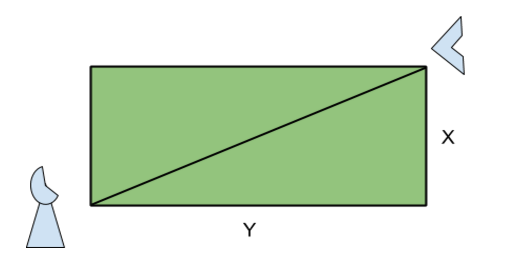
\includegraphics[width=0.8\textwidth]{figures/pic1.png}
  	\caption[Pipeline survey]{Scenario}
\end{figure}

Given the area of the rectangle we can compute the maximum distances of communication, which is the diagonal of the rectangle: 
\begin{equation*}\label{eq:scenario_parameters2} 
 		d_{max} = \sqrt{x^2 + y^2}
\end{equation*}
This distance will be taken into account when computing the radio link communication between the drone and GNS.


\chapter{Unmanned Aerial System Overview}\label{ch:uas}

Unmanned Aerial System, UAS, is the hardware responsible for keeping the connection between the ground station and the UA. However, when the distance between these two elements increases, the quality of the signal that is received and sent by both antennas is reduced. Therefore, it is essential to have the proper physical infrastuctures to be able to detect both strong and weak signals. These infrastuctures constitute the hardware and they cover every element connected with the vehicle, in the air, and the ground station, on the ground.

%However, increasing of the distance will reduce the quality of the signal that is received and sent by both antennas. In order to keep the communication, it is essential to have the proper physical infrastuctures to be able to detect both strong and weak signals. These infrastuctures constitute the hardware and they cover every element connected with the vehicle, in the air, and the ground station, on the ground. The previous description of the system as a whole constitutes the Unmanned Aerial System, UAS.

The UAS illustrated in Figure \ref{fig:uas} can be decomposed in the following elements:
\begin{itemize}
	\item Unmanned Aerial Vehicle, UAV
	\item Ground Station, GS
	\item Antennas
	\item Mission sensors
\end{itemize}

\begin{figure}[H]
	\centering
	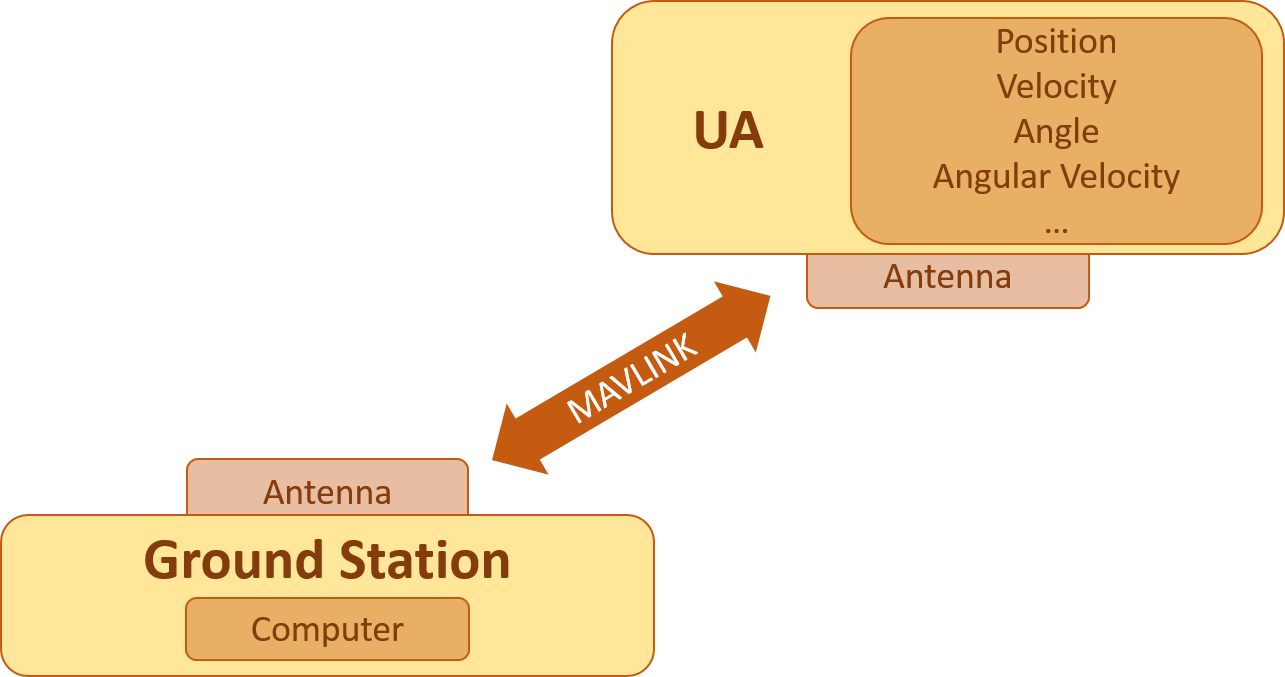
\includegraphics[scale=0.4]{figures/uas.png}
	\caption{Unmanned Aerial System}
	\label{fig:uas}
\end{figure}

%In order to have some bounds of the system we can have a look at the drone performances:
%\begin{itemize}
%	\item 50 km/h - stability at high speeds 
%	\item 40 minutes - battery autonomy (30 minutes with payload)
%	\item 2400 m - maximum flight altitude (higher if take off from mountain site)
%	\item 50 km - maximum radio communication (with directional antennas)
%	\item under 1 m - absolute positioning of X-Y GPS
%	\item GPS return-to Home (automatically activates when radio link is lost)
%\end{itemize}



\section{Unmanned Aircraft}\label{sec:drone}

The unmanned aircraft, UA, commonly called drone, is a vehicle, that to be piloted, doesn't need a person inside of it. Thus, it is necessary to have a system which is able to control the UA in order to accomplish the desired task. This system gives partial or total autonomy to the aircraft, meaning that it can be, respectively, a remote control from an operator or on-board computers prepared to act depending on different situations. The remote control from an operator can be either on the ground, in a GS, either in the air, in another vehicles.

Nowadays, the use of UAs is increasing due to the various tasks that they can perform, as surveillance, mapping, aerial photography, monitoring and military applications.

In this project, the operator will be on the ground and the UA will be controlled by a couple of tracking antennas. One antenna will be on-board the aircraft and the other will be on the ground on a base station which will receive and send information from and to the aircraft. 

For this project, eBee will be used as an example and can be observed in Figure \ref{fig:ebee}. This drone was developed by the company senseFly and has three different models: eBee, the mapping drone, eBee RTK, the survey-grade mapping drone and eBee Ag, the precision agriculture drone. Each model was created for a specific task, however the main characteristics are common to every model. The weight of this aircraft varies between 0.69 Kg and 0.73 Kg, the wingspan is 96 cm and they are made of EPP foam and carbon. They are equipped with a 11,1 V battery, which allows a flight time between 40 and 50 minutes, and with a WX camera (18.2 MP) which can be changed by another cameras like the thermoMAP. The thermoMAP captures thermal videos and still images which allows the creation of a full thermal map of a site. The Ground Sampling Distance (GSD), that is the distance measured on the ground between the center of two consecutive pixels when the picture was taken from the air, varies between 1.5 cm and 2 cm (maximum values). 
 
\begin{figure}[H]
  \centering
  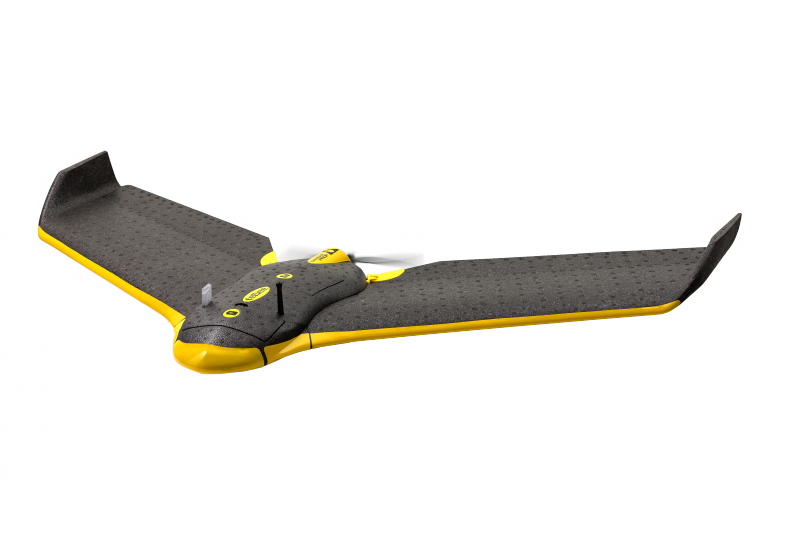
\includegraphics[scale=0.45]{figures/eBee.png}
  %\caption[The professional mapping drone eBee]
   %{The professional mapping drone \textit{eBee} \href{https://www.sensefly.com/drones/ebee.html}{(www.sensefly.com)}. Fully autonomous drone to capture high-resolution aerial photos that can transform into accurate 2D orthomosaics \& 3D models.}
   \caption{Commercial Drone \textit{eBee} \cite{eBee}.}
   \label{fig:ebee}
\end{figure}

The accuracy related to the position depends on the existence of ground control points (GCP). In the table \ref{accuracy} the vertical and horizontal accuracy for each model are described.

\begin{table}[h!]
	\centerline{
	\begin{tabular}{|c||c|c|c|}
		\hline
		Parameter & eBee & eBee RTK & eBee Ag\\ \hline\hline
		Horizontal Accuracy (with GCPs) & Down to 3 cm & - & Down to 4 cm\\ \hline
		Vertical Accuracy (with GCPs) & Down to 5 cm & - & Down to 7 cm\\ \hline
		Horizontal Accuracy (without GCPs) & 1-5 m & Down to 3 cm & 1-5 m\\ \hline
		Vertical Accuracy (without GCPs) & 1-5 m & Down to 5 cm & 1-5 m\\ \hline
	\end{tabular}}
	\caption{GPC Accuracy of the eBee models.}
	\label{accuracy}
\end{table}

The software that is responsible for controlling and planning the flight is called eMotion. This is a GS software and is supplied with every eBee model.
\section{Ground Station}\label{sec:gs}

The ground station is, generally, a terrestrial radio station designed for planetary and extraplanetary telecommunication with aircrafts and spacecrafts, respectively. For planetary telecommunications, the ground stations are located on the surface of the Earth and they communicate with the aircrafts by sending and receiving radio waves in a specific band of the spectrum. When a ground station successfully transmits radio waves to an aircraft or vice versa, it establiches a telecommunication link.

In the case this project, the ground station is prepared to control the UA using an antenna and a computer to communicate, analyse the received data and send commands to the aircraft. As was described in the section \ref{sec:drone}, in order to accomplish the desired task, the eBee was taken as an example. The monitorization of the movement of this aircraft is done using the eMotion software that is installed in the base station computer.

eMotion is a software that enables the user to plan, simulate, monitor and control the movement of the UA. In the planning part it is possible to import the background map and to draw a polygon that will correspond to the area that the user wants to cover. Then the user needs to define some parameters, like the ground resolution, and the eMotion will automatically generate a full flight plan, calculating the eBee’s required altitude and displaying its projected trajectory. It is also possible to correct some parameters of the generated trajectory that were not taking into account in the previous case, allowing, for instance, a fly over an uneven terrain.

Before the flight, it is possible to simulate the trajectory of the UA using eMotion's simulator. The simulation helps the user to understand how the camera will work during the flight and how will be the movement of the UA, without putting the aircraft at risk. After the simulation, while the vehicle is flying, eMotion provides a real-time information displaying all the flight parameters, the battery level and the image acquisition progress. During the flight, it is possible to manually control the UA using a tool that is available in this software. Every mistake can be corrected allowing the reconfiguration of the vehicle's flight plan and the landing point. Hence, this system allows a versatile control of the aircraft from the plan of the trajectory until the control during the flight.
\section{Antennas}\label{sec:antennas}

As it was mentioned before the often approach to this kind of communication is to use directional antennas.
The reason to do this, is that a directional antennas are known for having a very high gain in a narrow beam width, whereas on the other hand, an omnidirectional antenna has a lower gain while having a very broad beam width.
Therefore, the use of this first type of antennas will allow us to improve the quality of the radio link as long as the antennas are pointing at each other.

The antennas used for the GS and the UA are different by means of weight and size. The preference of using them is based on the application at hand, thus for:
\begin{itemize}
	\item GS - Parabolic (grid) directional antenna 
	\item UA - Patch directional antenna
\end{itemize}

A parabolic antenna in an antenna that uses a parabolic reflector and a curved surface to direct the radio waves and its main advantage is that it has a high directivity. This type of antennas are able to produce a narrow beam width which allow them to have some of the highest gains Parabolic antennas, due to their high gain, are intensively used for carry telephone and television signals between nearby cities.

Patch antenna, which is the original type of microstrip, is a low profile antenna that can be mounted on a flat surface and it consists in a rectangular sheet of metal. These antennas are very useful because they are very thin and they provide a quite high directivity.

Later on, in chapter \ref{ch:model} a modelling process to simulate these types of directional antennas will be addressed.
\section{DC Servomotor}\label{sec:servo_motor}

The control of both antennas requires the use of four motors which will be able to change its orientation (two motors per antenna in order to control two different angles). In this project, the DC servomotor was chosen because it can be either a rotary or a linear actuator which allows a precise control of angular or linear position, velocity and acceleration.

The servomotor can be described in two different parts: an electrical motor and a servomechanism. The electrical motor is a DC motor which is able to convert electrical power into rotational mechanical power and the servomechanism is the group of elements connected with the DC motor. The shaft of the DC motor is coupled with another shaft denominated output shaft. The connection is made through a gear assembly which is not only responsible for the connection between both shafts, but also for the reduction of the RPM of the motor’s shaft (figure \ref{servomotor_expl1}).

\begin{figure}[H]
\centering
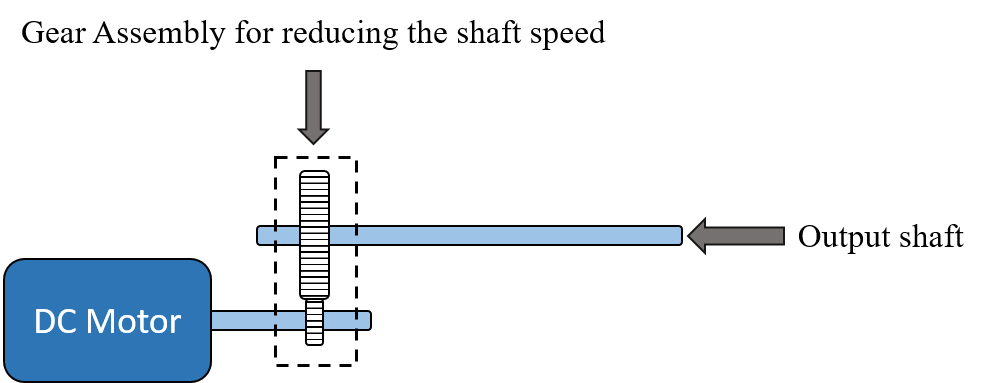
\includegraphics[scale=0.7]{figures/servomotor_expl1.png}
\caption{Connection between the output shaft and the DC motor}
\label{servomotor_expl1}
\end{figure}

The output shaft is also connected with a potentiometer by another gear assembly and, during its rotation, the knob rotates and creates an electrical signal. This signal increases proportionally with the angular movement of the potentiometer knob. The connection between the output shaft and the potentiometer can be
observed in the figure \ref{servomotor_expl2}.

\begin{figure}[H]
\centering
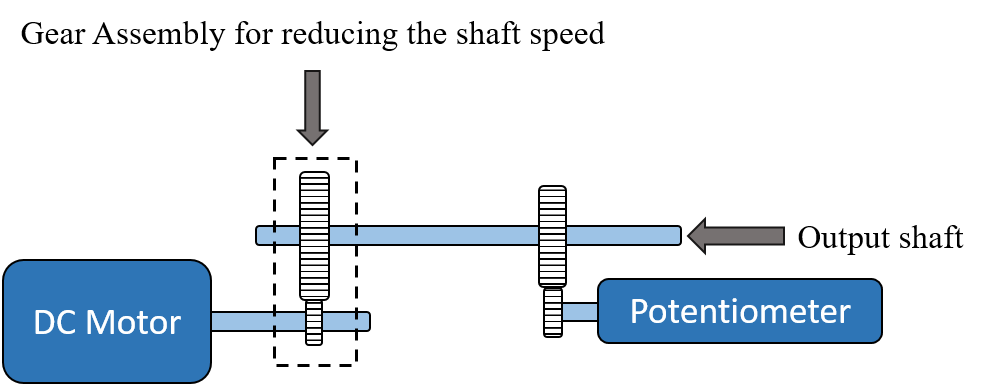
\includegraphics[scale=0.61]{figures/servomotor_expl2.png}
\caption{Connection between the output shaft and the potentiometer}
\label{servomotor_expl2}
\end{figure}

The previous described gears are involved in the gear mechanism which is responsible for the transformation of the original input speed provided by the DC motor into a slower output speed which is practical and widely applicable. 

The potentiometer is also connected with an error detector feedback amplifier where the electrical potential (from the potentiometer) and the input command voltage (the signal that represents the desired angle) are compared. The output of the error detector amplifier is called electrical input of the DC motor and is represented in the figure \ref{servomotor_expl3}. When the electrical potential equals the input voltage, which means that the shaft is in the desired position, the input of the DC motor becomes zero and the motor stops rotating until the next command.

\begin{figure}[H]
\centerline{
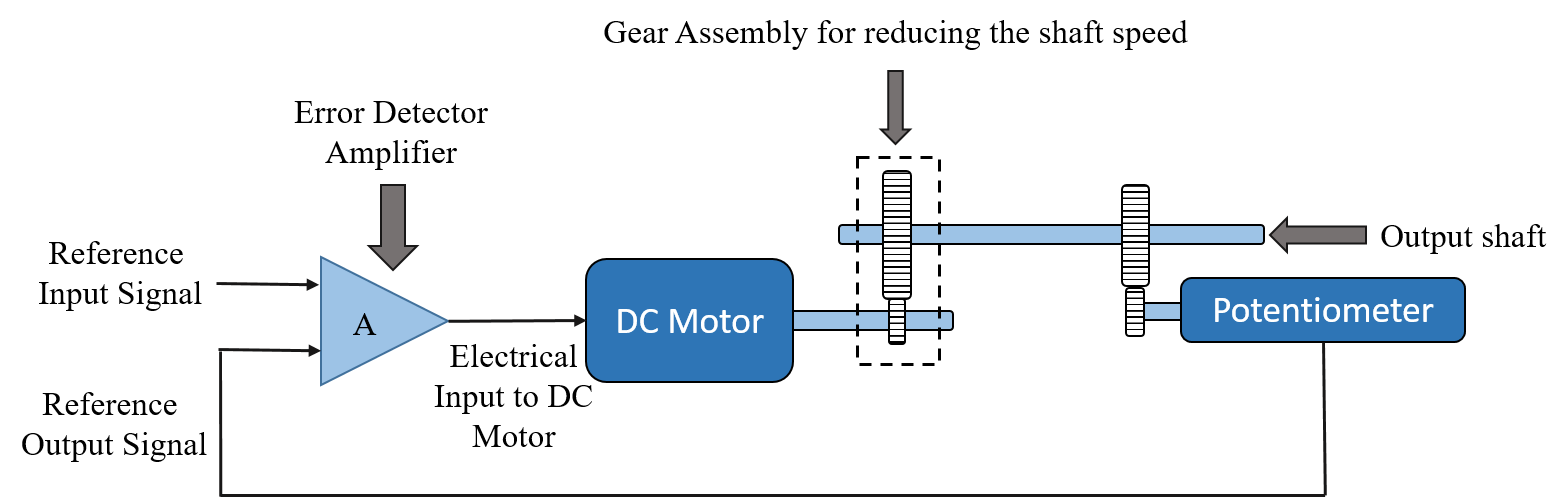
\includegraphics[scale=0.6]{figures/servomotor_expl3new.png}}
\caption{Servomotor’s feedback}
\label{servomotor_expl3}
\end{figure}

In order to be able to do the procedure described in the figure \ref{servomotor_expl3} it is necessary to apply a restricted input voltage signal in regular intervals. Servomotors operate from 4.8V to a 6V supply voltage, but 5V is the typical value. On the other hand, the pulse should have a specific width (PWM – Pulse Width Modulation) because it will be responsible for the amount of rotation. Typically, the duration of the pulse varies from 1ms to 2.2ms and the frequency from 50Hz to 60Hz. The size of the pulse will result in a lesser or greater rotation. The figure \ref{signal_servo} is an example of the relation pulse-rotation and describes three different cases. For instance, if the duration of the pulse is 1.25ms, the servomotor will rotate 90 degrees.

\begin{figure}[H]
\centering
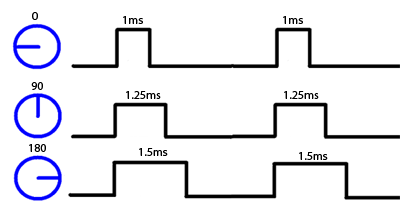
\includegraphics[scale=0.5]{figures/signal_servo.jpg}
\caption{Examples of the relation between the PWM and the rotation}
\label{signal_servo}
\end{figure}

Based on the previous explanation, the servomotor requires a power supply unit and the information about the rotation that should be done through an electrical signal. Hence, this motor needs three different terminals (the figure \ref{cable_servo} is one example of the terminals of a servo motor):
\begin{itemize}  
        \item Orange - Position signal (PWM pulses).
        \item Brown - $V_{cc}$ (from the power supply unit). 
        \item Red - Ground.
\end{itemize}

\begin{figure}[H]
\centering
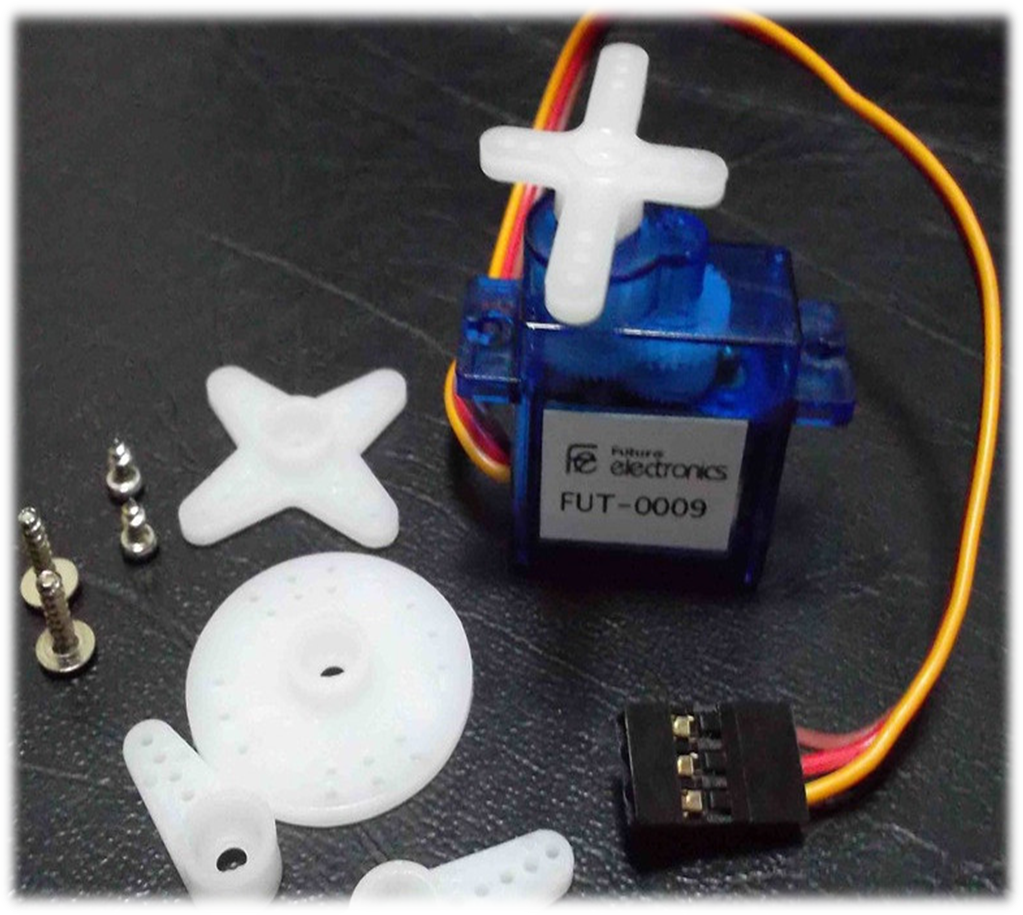
\includegraphics[scale=0.5]{figures/cable_servo.png}
\caption{Servo motor with its three different terminals}
\label{cable_servo}
\end{figure}



\chapter{Frames}\label{ch:frames}

In navigation, guidance, and control of an aircraft or rotorcraft, there are several
coordinate systems (or frames) intensively used in design and analysis. For ease of references, in this chapter the coordinate systems adopted in this project have been sumarized, which include:

\begin{itemize}
\item{The Geodetic Coordinate System}
\item{The Earth-Centered Earth-Fixed (ECEF) Coordinate System}
\item{The local North-East-Down (NED) Coordinate System}
\item{The vehicle-carried NED Coordinate System}
\item{The Body Coordinate System}
\end{itemize}

The relationships among these coordinate systems, i.e., the coordinate transformations, are also introduced. We need to point out that small UAs are normally used at low speeds in relatively small regions (non trans-oceanic travels), due to their inherent mechanical design and power limitation. This is crucial to some simplifications made in the coordinate transformation, e.g., omitting unimportant items in the transformation between the local NED frame and the body frame. For the same reason, partial transformation relationships provided in this chapter are not suitable for describing flight situations in which the rotation of the Earth is taken into account.
\section{Geodetic Coordinate System}\label{sec:coord}

\begin{figure}[H]
   \centering
    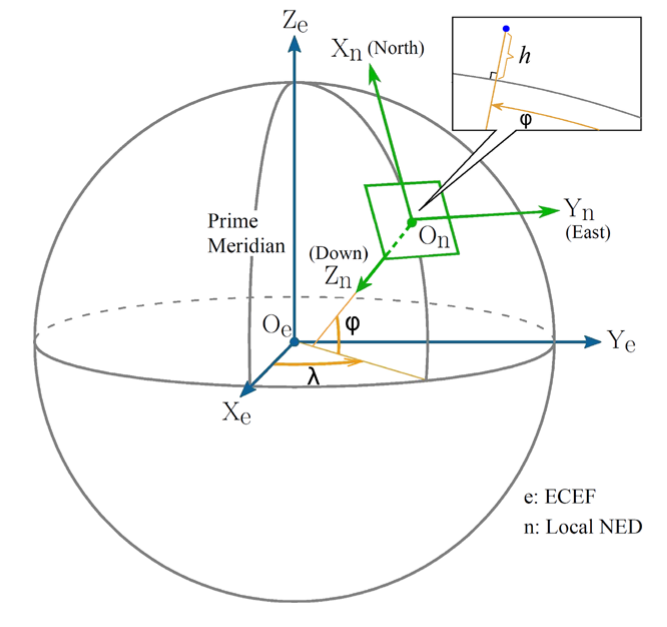
\includegraphics[width=.70\textwidth]{figures/GeoTemp1.png} 
    \caption{Geodetic, ECEF and local NED Frames.}  
    \label{fig:Geodetic1}
\end{figure}

\paragraph{}The geodetic coordinate system is widely used in GPS-based navigation. Note that it is not an usual Cartesian coordinate system but a system that characterizes a coordinate point near the earth’s surface in terms of longitude, latitude, and altitude (or height), which are respectively denoted by $\lambda$, $\varphi$, and h (yellow lines) in figure \ref{fig:Geodetic1}.

\paragraph{}The \textit{World Geodetic System} is a standard used in cartography, geodesy and navigation. This standard sets reference points based on an ellipsoidal model of the earth and a gravitational equipotential surface that defines the nominal sea level. Its latest version is \textbf{WGS84}, and that is the one used throughout this project. 

The longitude measures the rotational angle (ranging from $-180$ to $180$ degrees) between the Prime Meridian and the measured point. The latitude measures the angle (ranging from $-90$ to $90$ degrees) between the equatorial plane and the normal of the reference ellipsoid that passes through the measured point. The height (or altitude) is the local vertical distance between the measured point and the reference ellipsoid.

\paragraph{}Thanks to the \textbf{WGS84} standard a list of parameters can be defined that will help us transform the Geodetic Frame to other Coordinate systems:

\begin{itemize}
\item{Semi-major axis\\
\begin{align*}
& R_{Ea} = 6378137.0 \text{ m}
\end{align*}}
\item{Flattening factor\\
\begin{align*}
& f = 1/298.257223563 
\end{align*}}
\item{Semi-minor axis \\
\begin{align*}
& R_{Eb} = R_{Ea}(1-f) = 6356752.0 \text{ m}
\end{align*}}
\item{First Eccentricity \\
\begin{align*}
& \textbf{e} = \frac{\sqrt{R_{Ea}^2-R_{Eb}^2}}{R_{Ea}} = 0.08181919
\end{align*}}
\item{Meridian radius of curvature \\
\begin{align*}
& M_{E} = \frac{R_{Ea}(1-\textbf{e}^2)}{(1-\textbf{e}^2\sin^2\varphi)^{3/2}} 
\end{align*}}
\item{Prime vertical radius of curvature \\
\begin{align*}
& N_{E} = \frac{R_{Ea}}{\sqrt{(1-\textbf{e}^2\sin^2\varphi)}}
\end{align*}}
\end{itemize}

\section{WGS84}\label{sec:wgs}
\section{North-East-Down (NED) Coordinate System}\label{sec:ned}

\paragraph{} The North-East-Down is a geographical coordinate system fixed to the Earth's surface, and, precesily because of this, is also known as \textbf{local tangent plane (LTP)} or ground coordinate system (green lines in Figure \ref{fig:Geodetic1}). The origin and axis of this system are defined as follows: 
\begin{itemize}
\item{The origin (\textbf{$O_{n}$}) is located at a arbitrary point on the Earth's surface.}
\item{The X-axis (\textbf{$X_{n}$}) points towards the geodetic north.}
\item{The Y-axis (\textbf{$Y_{n}$}) points towards the geodetic east.}
\item{The Z-axis (\textbf{$Z_{n}$}) points downward along the ellipsoidal normal, set by the right-hand rule.}
\end{itemize}

\paragraph{} The local NED frame plays a very important role in flight control and navigation.
Navigation of small-scale UAVs is normally carried out within this frame. It will later be shown that during this work 2 different local NED frames would be described. One being with the origin fixed at the Ground Station location and one with an origin at the center of gravity of the UAV at all times. This is the so-called \textbf{Vehicle-carried NED}, represented with the \textit{nv} subscript in Figure \ref{fig:NED1}.\\
Note that, strictly speaking, the axis of the Vehicle-carried NED are not completely aligned with with the ones of the local NED , varying due to the movement of the vessel. However, for smalls aircrafts the directional difference is completely neglectable. Furthermore, $h = -z$ is often used to denote the actual height of the UAV.

\paragraph{} Now, to define a point within this local frame, spherical coordinates will be used. In mathematics, a spherical coordinate system is a coordinate system for three-dimensional space where the position of a point is specified by three numbers: the \textbf{radial distance} of that point from a fixed origin ($\rho$), its \textbf{polar angle} measured from a fixed zenith direction ($\theta$), and the \textbf{elevation angle} of its orthogonal projection on a reference plane, measured from a fixed reference direction on that plane ($\phi$).\\
The way these spherical coordinates are defined during this specific project are shown in Figure \ref{fig:Spherical1}.
\begin{figure}[H]
   \centering
    \includestandalone[width=.60\textwidth]{figures/3D_Sphcoord} 
    \caption{Spherical Coordinates}
    \label{fig:Spherical1}
\end{figure}

\paragraph{} Note how this cartesian coordinate system is defined such that $\theta = 0$ is aligned with the east ($y$) axis of the NED frame and  $\phi > 0$ is defined for negative values or $z$, i.e., positive height on the surface of the Earth.
Additionally, it is necessary to define a unique set of spherical coordinates for each point, and therefore restricting the range of these parameters is required. In our case the coordinates will be limited as follows:
\begin{align*}
& \rho \geq 0 \\
& -\pi \leq \theta < \pi \\
& \frac{-\pi}{2} \leq \phi \leq \frac{\pi}{2}
\label{eq:los_distToHorizon}
\end{align*}
These constraints define the conversion between Cartesian and Spherical coordinates such that:
\begin{align*}
x &=  \rho\cos\phi\sin\theta  & \rho &= \sqrt{x^{2} + y^{2} + z^{2}} \\
y &= \rho\cos\phi\cos\theta   & \theta &= \arctan\left(x\right)\\
z &= \rho\sin\phi       & \phi &=  \arctan\left(-z\right)
\label{eq:los_distToHorizon}
\end{align*} 


\section{Body Coordinate System}\label{sec:body}
This frame has also the origin in the center of gravity of the UA, however, unlike the vehicle-carried NED, the axis rotate with the craft:
\begin{itemize}
\item{The origin (\textbf{$O_{b}$}) is located at the center of gravity of the UA.}
\item{The X-axis (\textbf{$X_{b}$}) points in the forward direction.}
\item{The Y-axis (\textbf{$Y_{b}$}) points towards starboard, the right side of the UA.}
\item{The Z-axis (\textbf{$Z_{b}$}) points downward, set by the right-hand rule.}
\end{itemize}
\begin{figure}[H]
   \centering
    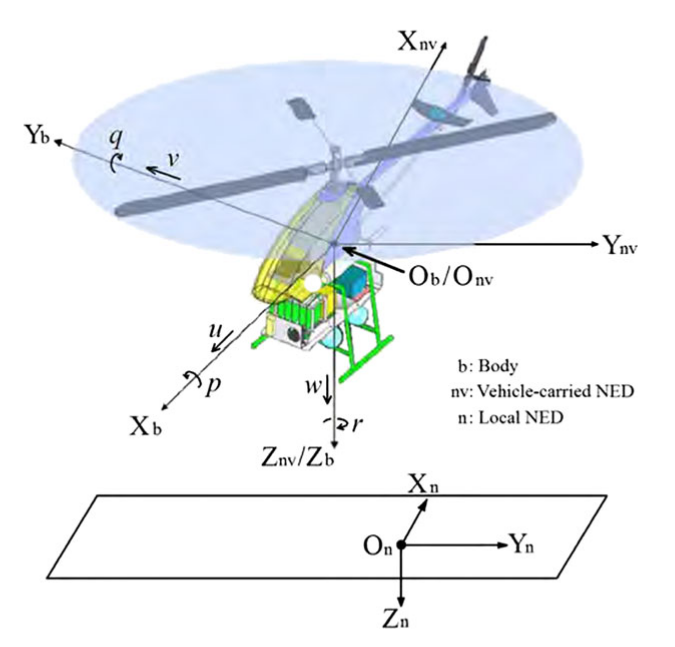
\includegraphics[width=.70\textwidth]{figures/NEDtemp1.png} 
    \caption{Body, vehicle-carried and local NED Frames.\cite{Cai011}}  
    \label{fig:NED1}
\end{figure}

\section{Transformations}\label{sec:body}

\subsection*{From NED to Body}
\paragraph{} The orientation of a Cartesian coordinate system with respect to another can be described in three successive Euler rotations, usually performed about each of the three cartesian axes consequently. During this work we will mainly focus on the transformation between the vehicle-carried NED and the body frame. In order to do this we will follow a specific rotation sequence, moving the reference frame to the referred frame by a Z-Y-X (also called 3-2-1) sequence. These three Euler angles are also known respectively as \textbf{yaw}($\psi$), \textbf{pitch}($\xi$) and \textbf{roll}($\gamma$)\cite{EulerW}.

\paragraph{} This way, the transformation from the vehicle-carried NED frame to the Body frame is given by:
\begin{align}
\textbf{P}_{b} = \textbf{R}_{b/nv}\textbf{P}_{nv}
\end{align}
where \textbf{R}$_{b/nv}$ is the \textbf{Rotation matrix}:
\begin{align*}
\textbf{R}_{b/nv} =
\begin{bmatrix}
c(\xi)c(\psi) & c(\xi)s(\psi) & -s(\xi)\\
s(\gamma)s(\xi)c(\psi) - c(\gamma)s(\psi) & s(\gamma)s(\xi)s(\psi) + c(\gamma)c(\psi) & s(\gamma)c(\xi)\\
c\gamma)s(\xi)c(\psi) + s(\gamma)s(\psi) & c(\gamma)s(\xi)s(\psi) - s(\gamma)c(\psi) & c(\gamma)c(\xi)
\end{bmatrix}
\end{align*}

\paragraph{} However, even though the local NED coordinates is what is necessary to transform to the Body frame, the only available resource  is the GPS position measurements of each of our devices (Ground station and UA). Therefore a transformation from Geodetic Coordinate Frame to local NED frame is in due. The ECEF Coordinate Frame will be used as an intermediate step during this process.

\subsection*{From Geodetic to ECEF}
Being \textbf{P}$_{g}$ the position of a point in the geodetic system such that is defined by its latitude, longitude and height:
\begin{align}
\textbf{P}_{g} = 
\begin{bmatrix}
\lambda \\
\varphi\\
h
\end{bmatrix}
\end{align}
By using the parameters set by the \textbf{WGS84} standard in Section \ref{sec:geodetic} the transformed point, \textbf{P}$_{e}$ will be given by
\begin{align}
\textbf{P}_{e} = 
\begin{bmatrix}
\lambda \\
\varphi\\
h
\end{bmatrix}
=
\begin{bmatrix}
(N_{E}+h)c(\varphi)c(\lambda) \\
(N_{E}+h)c(\varphi)s(\lambda) \\
(N_{E}(1-\textbf{e}^2)+h)s(\varphi)
\end{bmatrix}
\end{align}

\subsection*{From ECEF to NED}
Analogously to the former transformation, we have
\begin{align}
\textbf{P}_{n} = \textbf{R}_{n/e}\left(\textbf{P}_{e} - \textbf{P}_{e,ref}\right)
\end{align}
where \textbf{P}$_{e,ref}$ is the position of the origin of the local NED frame in ECEF frame and \textbf{R}$_{n/e}$ is the \textbf{Rotation matrix} given by: 
\begin{align*}
\textbf{R}_{n/e} =
\begin{bmatrix}
-s(\varphi_{ref})c(\lambda_{ref}) & -s(\varphi_{ref})s(\lambda_{ref}) & c(\varphi_{ref})\\
-s(\lambda_{ref}) & c(\lambda_{ref}) & 0\\
-c(\varphi_{ref})c(\lambda_{ref}) & -c(\varphi_{ref})s(\lambda_{ref}) & -s(\varphi_{ref})\\
\end{bmatrix}
\end{align*}
where $\varphi_{ref}$ and $\lambda_{ref}$ are the latitude and longitude of the reference point in Geodetic frame.

\chapter{Telecommunication}\label{ch:telecommunication}

Drone communication links are generally either radio frequency (RF) or lasercom (optical). Even though both types currently suffer from bandwidth limitations, lasercom could surpass RF in terms of airborne data transfer rate. However, RF will continue to dominate at the lower altitudes for some time into the future because of its better all-weather capability. Additionally, RF links have the advantage of being much more efficient and usually much less complex than lasercom links.
Data rates for RF links have traditionally been restricted due to limited spectrum and
minimization of communication system size, weight, and power.

Radio waves are a form of electromagnetic radiation with frequencies ranging from 3 kHz to 300 GHz. The size and profile constraints of small drones cannot facilitate communication links on the low-frequency (large wavelength) end of the spectrum. 
On the other hand, atmospheric attenuation as well as attenuation by rain, both
exponential in character, becomes a serious limiting factor to the link distance in
the millimeter wavelength region (>300MHz). 
	
Due to these limitations, small drone communication links are restricted to the very high frequency (VHF), the ultrahigh frequency (UHF), and rarely the super-high frequency (SHF) bands.

\section{Telemetry}
One of the main goal of drone surveillance is to procure relevant data. This is done by means of telemetry which is an automated communication process. In this process the data collected is transmitted to a receiving equipment for further processing and monitoring. 

!!! ADD MORE INFO !!!

!!! ADD FIGURE !!!

!!! HOW WE USE IT ? !!!

\section{MAVLink protocol}
When speaking of digital communication it is required to have a certain communication protocol. Given the fact that, this project deals with drones, a special protocol, namely Micro Air Vehicle Link (MAVLink) has been taken into consideration. This protocol is used in a GNS and drones scenario, where inter-communication between systems is needed in order to transmit GPS location, heading angle and speed.  

\subsection{Packet structure}
For further understanding the packet structure of such a protocol is needed as seen in Table \ref{tab:mavlink}.

\begin{table}[h]
	\centering
	\begin{tabular}{|c||c|c|}
		\hline
		Field name       & Index (Bytes)  & Purpose											     \\ \hline\hline
		Start-of-frame   &      0         & Start of frame transmission 							   \\ \hline
		Pay-load-length  &      1         & Length of payload (n)       							   \\ \hline
		Packet sequence  &      2    	  & Sent sequence counter (detect packet loss)                 \\ \hline
		System ID        & 		3		  & Sending system identification 							   \\ \hline
		Component ID     & 		4 		  & Sending component identification 						   \\ \hline
		Message ID       & 		5 		  & Message identification (correctly decoded)      		   \\ \hline
		Payload          &   6 to (n+6)   & Data into the message, depends on Message ID        	   \\ \hline
		CRC              & (n+7) to (n+8) & Check-sum of packet (excluding packet start sign)          \\ \hline
	\end{tabular}
	\caption{MAVLink packet structure}
	\label{tab:mavlink}
\end{table}

The CRC field ensures message integrity of each packet. Another function of the CRC is to establish that both sender and receiver agree on the message transfer. Additionally, a seed value is appended at the end of the data when computing the CRC, generated with every new message.

\subsection{Messages}
As stated above the payload from the packets are MAVLink messages. Also, every message can be identified by its ID field on the packet. Additionally, an XML document (in MAVLink source) has the definition of all the data stored on that payload. A sample of such an XML document can be seen in Figure \ref{fig:mav_msg} which describes a message with an ID 24 giving GPS relevant information.

\begin{figure}[h]
	\centering
	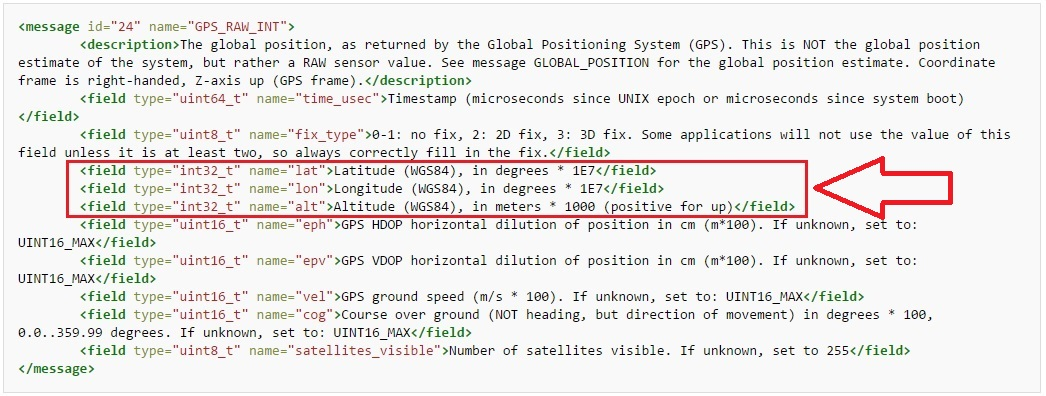
\includegraphics[scale=0.5]{figures/mavlink_msg.jpg}
	\caption{MAVLink message XML document}
	\label{fig:mav_msg}
\end{figure}

To be noted that the XML document describes the logical ordering of the fields for the protocol, not the actual wire format.


\section{Compute Link Budget}

\subsection{Line-Of-Sight Propagation}\label{subsec:los_propagation}
At low frequency (below approximately 3 MHz) radio signals travel as ground waves, which follow the Earth's curvature due to diffraction with the layers of the atmosphere.
However, at higher frequencies and in lower levels of the atmosphere, neither of these effects are significant. Thus any obstruction between the transmitting antenna (transmitter) and the receiving antenna (receiver) will block the signal, just like the light that the eye may sense. Therefore, since the ability to visually see a transmitting antenna (disregarding the limitations of the eye's resolution) roughly corresponds to the ability to receive a radio signal from it, the propagation characteristic of VHF and higher radio frequency (>30 MHz) paths is called line-of-sight. The farthest possible point of propagation is referred to as the radio horizon.

The radio horizon is the locus of points at which direct rays from an antenna are tangential to the surface of the Earth. If the Earth were a perfect sphere and there were no atmosphere, the radio horizon would be a circle.
This way the greatest distance at which a receiver can see the transmitter is explained in the following paragraph.

First, we are going to derive a general expression and after that apply it to a scenario with a drone and a basestation. In figure  \ref{fig:GeometricDist_general} the relationship between the height of the observer above sea level (O point) and the distance d which is between it and the horizon (H point) is shown. Finding this distance is done by the use of the pythagorean theorem. With some simple mathematical calculations the distance d is derived in the following:

\begin{equation}\label{eq:los_distToHorizon}
	(R+h)^2 = R^2+d^2\nonumber \\
	\Rightarrow R^2+2hR+h^2 = R^2+d^2 \Rightarrow d^2 = 2hR + h^2 \\
	\Rightarrow d = \sqrt{2hR + h^2}
\end{equation} 

\begin{figure}
    \hfill
    \subfigure[Geometrical distance to the horizon]{
    	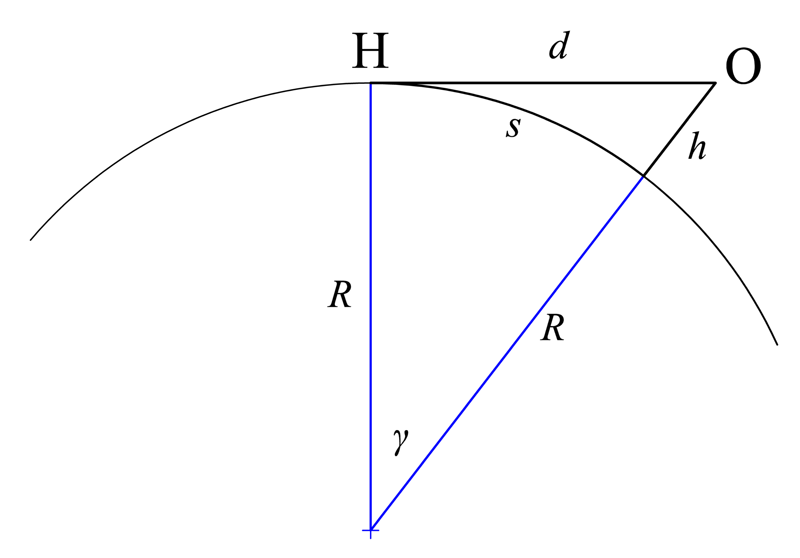
\includegraphics[scale=4]{figures/GeometricDistanceToHorizonOneTriangle.png} 
		\label{fig:GeometricDist_general}}
	\hfill
    \subfigure[Geometrical distance from drone to GNS]{
    	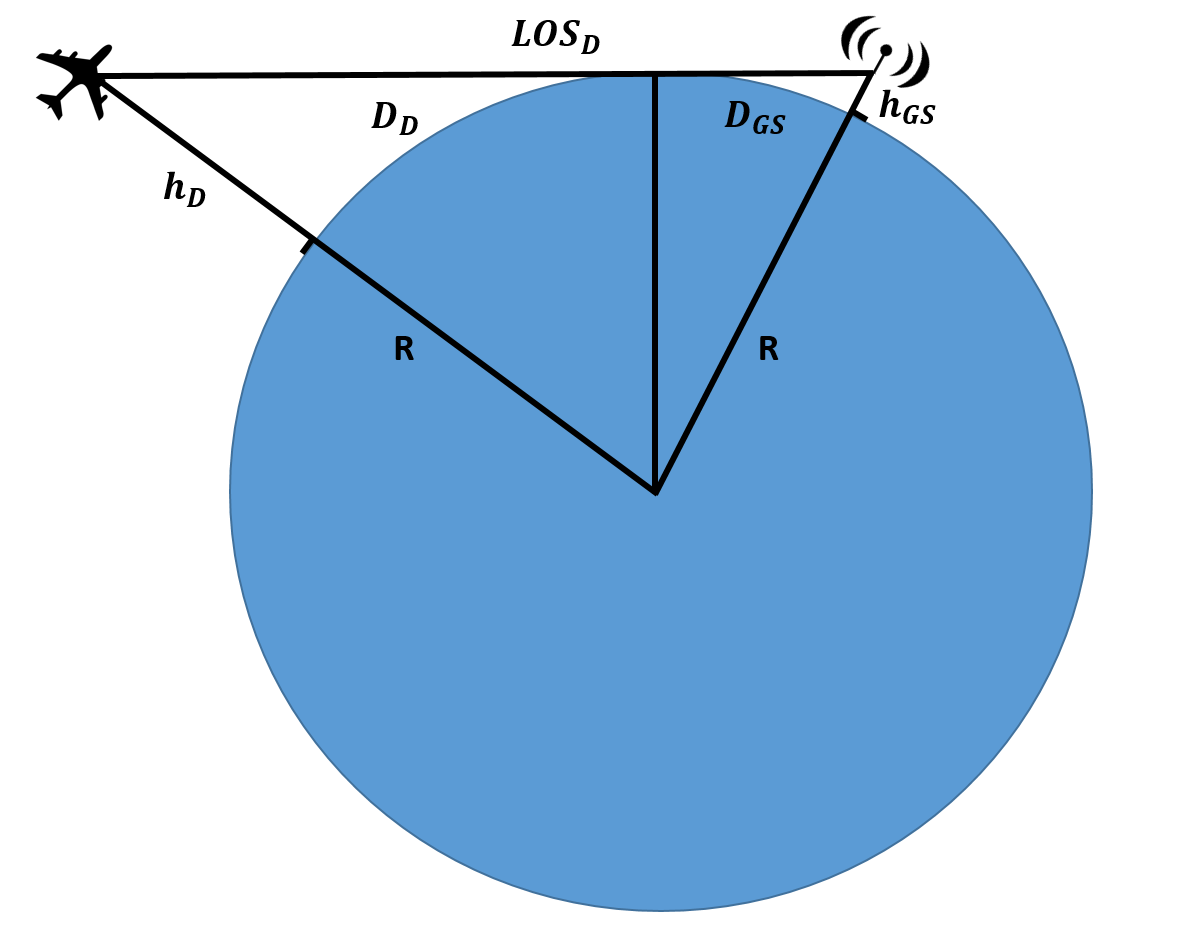
\includegraphics[scale=0.3]{figures/GeometricDistanceToHorizonTwoTriangle.png} 
    	\label{fig:GeometricDist_droneBasestation}}
    \hfill
    \caption{Geometrical distance to the horizon, Pythahorean theorem}
\end{figure}

On figure \ref{fig:GeometricDist_droneBasestation} it is shown that the two objects are a drone and a basestation. Both of them wont be higher then approx 100 meter and since R is radius of the Earth, $2hR$ >> $h^2$ and $h^2$ is therefore neglected in equation \ref{eq:los_distToHorizon}. The two distances $D_D$ and $D_B$ have the same expressions in both cases:
\begin{align*}
	D_D [km] &= \sqrt{2\cdot R \cdot h_D + h_{D}^2} \approx \sqrt{2\cdot 6.378\cdot h_D} = \sqrt{12.756\cdot h_D} = 3.57\cdot \sqrt{h_D} \\
	D_B [km] &= \sqrt{2\cdot R \cdot h_B + h_{B}^2} \approx \sqrt{2\cdot 6.378\cdot h_B} = \sqrt{12.756\cdot h_B} = 3.57\cdot \sqrt{h_B}
\end{align*}

To calculate the distance $D_{DB}$:
\begin{align}
	D_{DB}[km]	 &= D_D + D_B \approx 3.57\cdot \sqrt{h_D} + 3.57\cdot \sqrt{h_B} = {3.57\cdot (\sqrt{h_D} + \sqrt{h_B}} )
\end{align}

\subsection{Example with drone = 100m and basestation = 20m}
Lets take an example if the drone is at $h_D = 100m$ and the basestation at $h_B = 20m$. The distance between the drone and the basestation is as follows:
\begin{equation*}
	D_{DB}[km] = 3.57\cdot (\sqrt{100} + \sqrt{20}) = 51.67km
\end{equation*}

\subsection{Free space path loss}\label{subsec:path_loss}
\paragraph{}
The free space path loss (FSPL) is the loss in signal strength that occurs when an electromagnetic wave travels over a line of sight path in free space. In these circumstances there are no obstacles that might cause the signal to be reflected, refracted, or that might cause additional attenuation. Equation \ref{eq:path_losses} represents the loss in signal strength in dB.

\begin{equation}\label{eq:path_losses}
	L_{FS} = 20\lg\left (\frac{4\pi \cdot d}{\lambda} \right)
\end{equation}

The wave length can also be described by a relationship between the frequency and the velocity of light. This relationship is described by the equation \ref{eq:vel_freq_wavelen1}.

\begin{equation}\label{eq:vel_freq_wavelen1}
	\lambda = \frac{c}{f}
\end{equation}

Explanation of the parameters.
\begin{itemize}
	\item d - distance from transmitter to receiver [m]
	\item $\lambda$ - wavelength of the signal [m]
	\item c - speed of light constant $3\cdot 10^8$ [m/s] 
	\item f - frequency of signal [Hz]
\end{itemize}

Considering our problem we will look into the worst case scenario, which would be maximum distance between the GNS and the drone. 
\begin{equation*}
	Assume 
	\begin{cases}
	d_{max} = \sqrt{x^2+y^2}\\
	\text{f} = f\text{GHz (Should be permitted by law})\\
	\end{cases}
\end{equation*}

Computing signal wavelength:
\begin{equation}\label{eq:vel_freq_wavelen2}
	\lambda = \frac{c}{f} 
	        = \frac{3\cdot 10^{8}}{f\cdot 10^{9}}
	        = \frac{3}{10f}m
\end{equation}

Computing path loss:
\begin{align*}\label{eq:path_loses_calc}
	L = 20\lg\left (\frac{4\pi d}{\lambda} \right) dB 
	 &= 20\lg\left (\frac{4\pi \sqrt{x^2+y^2}}{\frac{3}{10f}} \right) dB\\ 
	 &= 20\lg\left (\frac{4\pi \sqrt{x^2+y^2}\cdot 10f}{ 3} \right) dB
\end{align*}
\noindent \textbf{As an observation, higher distance value between GNS and drone will result in higher path loss.}

\subsection{Link Budget}\label{subsec:link_budget}
\paragraph{}
A link budget is accounting of all of the gains and losses from the transmitter, through the medium  to the receiver in a telecommunication system. It accounts for the attenuation of the transmitted signal due to propagation, as well as the antenna gains, feedline and miscellaneous losses. 
\begin{equation*}\label{eq:link_budget} 
 		\text{Received Power (dBm)} = \text{Transmitted Power (dBm)} + \text{Gains (dB)} - \text{Losses(dB)}
\end{equation*}

In more detailed a common radio link looks like this:

\begin{equation*}\label{eq:link_budget} 
 		P_{RX} = P_{TX} + G_{TX} - L_{TX} - L_{FS} - L_{M} + G_{RX} - L_{RX}
\end{equation*}

Note that decibels are logarithmic measurements, so adding decibels is equivalent to multiplying the actual numeric ratios.


\section{Fresnel zones}
Taking into account that the application at hand involves radio communication it is important to talk about the Fresnel zones. Thus, it can be seen in Figure \ref{fig:fresnel_zones} the three Fresnel zones on the transmission path between A and B. 

\begin{figure}[h]
	\centering
	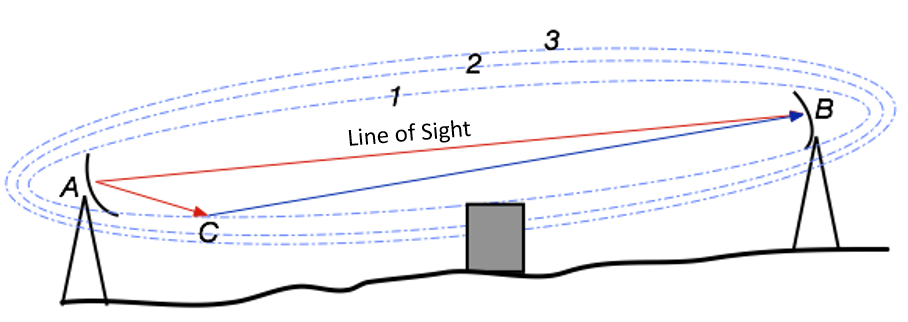
\includegraphics[scale=0.65]{figures/fresnel_zones.png}
	\caption{Fresnel zones between transmitter and receiver}
	\label{fig:fresnel_zones}
\end{figure}


ADD MORE RELEVEANT THINGS 

! ! ! ! \url{https://en.wikipedia.org/wiki/Fresnel_zone}  ! ! ! !


\section{Line-Of-Sight Propagation}\label{subsec:los_propagation}
\paragraph{}At low frequency (below approximately 3 MHz) radio signals travel as ground waves, which follow the Earth's curvature due to diffraction with the layers of the atmosphere.
However, at higher frequencies and in lower levels of the atmosphere, neither of these effects are significant. Thus any obstruction between the transmitting antenna (transmitter) and the receiving antenna (receiver) will block the signal, just like the light that the eye may sense. Therefore, since the ability to visually see a transmitting antenna (disregarding the limitations of the eye's resolution) roughly corresponds to the ability to receive a radio signal from it, the propagation characteristic of VHF and higher radio frequency (>30 MHz) paths is called \textbf{Line-Of-Sight}. The farthest possible point of propagation is referred to as the \textbf{radio horizon}.

\paragraph{}The radio horizon is the locus of points at which direct rays from an antenna are tangential to the surface of the Earth. If the Earth were a perfect sphere and there were no atmosphere, the radio horizon would be a circle.
This way the greatest distance at which a receiver can see the transmitter is explained in the following paragraph.

\paragraph{}First, we are going to derive a general expression and, after that, apply it to a scenario with a UA and a GS. In figure  \ref{fig:GeometricDist_general} the relationship between the height of the observer above sea level (O point) and the distance d which is between it and the horizon (H point) is shown. Finding this distance is done by the use of the pythagorean theorem. With some simple mathematical calculations the distance d is derived in the following:

\begin{equation}\label{eq:los_distToHorizon}
	(R+h)^2 = R^2+d^2\nonumber \\
	\Rightarrow R^2+2hR+h^2 = R^2+d^2 \Rightarrow d^2 = 2hR + h^2 \\
	\Rightarrow d = \sqrt{2hR + h^2}
\end{equation} 

\begin{figure}[H]
    \hfill
    \subfigure[Geometrical distance to the horizon]{
    	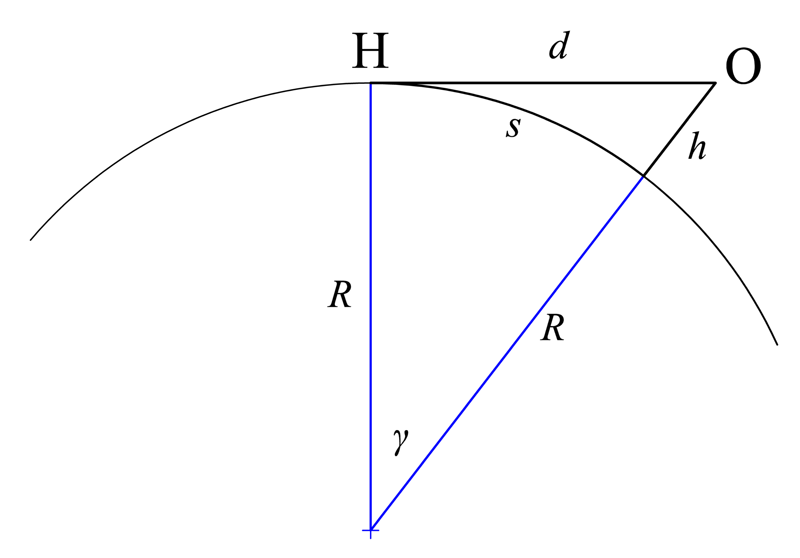
\includegraphics[scale=4]{figures/GeometricDistanceToHorizonOneTriangle.png} 
		\label{fig:GeometricDist_general}}
	\hfill
    \subfigure[Geometrical distance from UA to GS]{
    	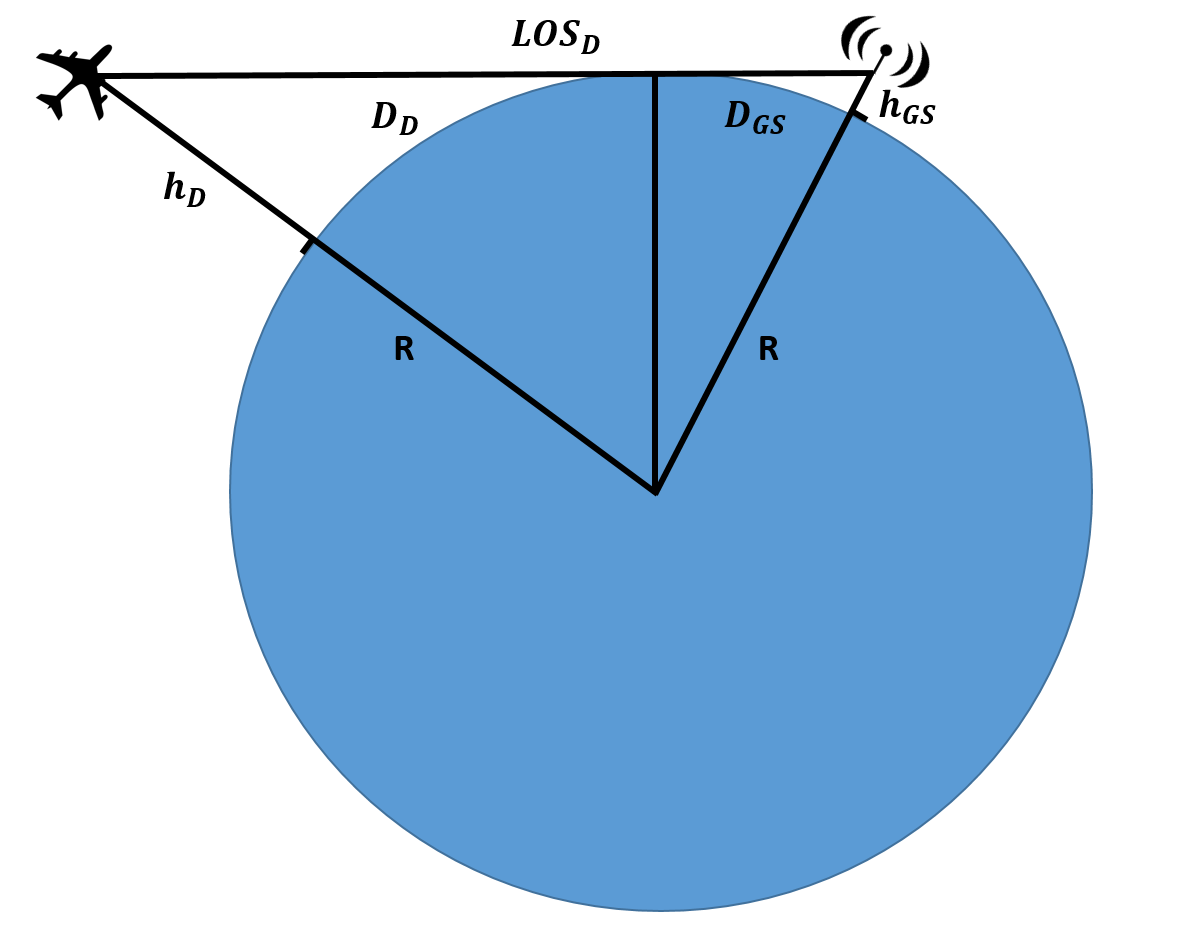
\includegraphics[scale=0.3]{figures/GeometricDistanceToHorizonTwoTriangle.png} 
    	\label{fig:GeometricDist_droneBasestation}}
    \hfill
    \caption{Geometrical distance to the horizon, Pythahorean theorem}
\end{figure}

On Figure \ref{fig:GeometricDist_droneBasestation} it is shown that the two objects are a GS and an UA. Both of them will not be higher then approx 100 meters and since R is radius of the Earth, $2hR$ >> $h^2$ and $h^2$ is therefore neglected in equation \ref{eq:los_distToHorizon}. The two distances $D_D$ and $D_{GS}$ have the same expressions in both cases:
\begin{align*}
	D_D [km] &= \sqrt{2\cdot R \cdot h_D + h_{D}^2} \approx \sqrt{2\cdot 6.378\cdot h_D} = \sqrt{12.756\cdot h_D} = 3.57\cdot \sqrt{h_D[m]} \\
	D_{GS} [km] &= \sqrt{2\cdot R \cdot h_{GS} + h_{GS}^2} \approx \sqrt{2\cdot 6.378\cdot h_{GS}} = \sqrt{12.756\cdot h_B} = 3.57\cdot \sqrt{h_{GS}[m]}
\end{align*}

Now, with these derivations, we can calculate the maximum distance at which both Ground Station and UA are still able to see each other ($LOS_{d}$), and therefore keep the communication.
\begin{align}
	LOS_d[km]	 &= D_D + D_{GS} \approx 3.57\cdot \sqrt{h_D[m]} + 3.57\cdot \sqrt{h_{GS}[m]} = {3.57\cdot (\sqrt{h_D[m]} + \sqrt{h_{GS}[m]}} )
\end{align}

\subsection*{LOS Distance Example}
A simple but realistic example scenario would be where the aircraft is at $h_D = 100$m and the ground station at $h_B = 20$m. This maximum distance between them is as follows:
\begin{equation*}
	LOS_d = 3.57\cdot (\sqrt{100} + \sqrt{20}) = 51.67 \text{ km}
\end{equation*}

During the course of this document this number might sometimes appear as an upper limit for the maximum distance since, further than that, there would not be Line-Of-Sight connection. Increasing this distance would be resulting from either increasing the altitude of the drone (which involves some law considerations) or of the Ground Station (which involves setting the Ground Station in a quite high building or mountain).





\section{Link Budget}\label{subsec:link_budget}
\paragraph{}
As the next step, once it is assured that there is Line-Of-Sight connection, it is important to calculate what is termed as the \textbf{Link budget}. This calculation is an accounting of all the gains and losses from the transmitter, through the medium,  to the receiver in a telecommunication system. It includes terms on it for the attenuation of the transmitted signal due to propagation, as well as the antenna gains, feedline and miscellaneous losses. It is precesily by assesing the link budget that is possible to design the system so that it meets the requirements and performs as desired. Its general form is:
\begin{equation*}\label{eq:link_budget} 
 		\text{Received Power (dBm)} = \text{Transmitted Power (dBm)} + \text{Gains (dB)} - \text{Losses(dB)}
\end{equation*}

And, in a more detailed look, it can divided down into:

\begin{equation*}\label{eq:link_budget} 
 		P_{RX} = P_{TX} + G_{TX} - L_{TX} - L_{FS} - L_{M} + G_{RX} - L_{RX}
\end{equation*}
where,
\begin{itemize}
\item{$P_{RX} -$ Recieved power [dBm]}
\item{$P_{TX} -$ Transmitter output power [dBm]}
\item{$G_{TX} -$ Transmitter antenna gain [dBi]}
\item{$L_{TX} -$ Transmitter feeder and associated losses (transmission line, connectors, etc.) [dB]}
\item{$L_{FS} -$ \textbf{Free Space Loss} or \textbf{Path Loss} [dB]}
\item{$L_{M} -$ Miscellaneus signal propagation losses (fading margin, polarization mismatch, other losses...) [dB]} 
\item{$G_{RX} -$ Receiver Antenna Gain [dBi]}
\item{$L_{RX} -$ Receiver feeder and associated losses (transmission line, connectors, etc.) [dB]} 
\end{itemize}
Note that losses are treated as possitive numbers and therefore they appear as a substraction in the link budget. Also highlight that decibels are logarithmic measurements, so adding decibels is equivalent to multiplying the actual numeric ratios.
 
\subsection{Free Space Loss}\label{subsec:path_loss}
\paragraph{}
The free space path loss is the loss in signal strength that occurs when an electromagnetic wave travels over a line of sight path in free space. In these circumstances there are no obstacles that might cause the signal to be reflected, refracted, or that might cause additional attenuation. Equation \ref{eq:path_losses} represents the loss in signal strength in dB.

\begin{equation}\label{eq:path_losses}
	L_{FS}\text{ [dB]} = 20\log\left (\frac{4\pi d}{\lambda} \right)
\end{equation}
where
\begin{itemize}
	\item d - Distance from transmitter to receiver [m]
	\item $\lambda  = \dfrac{c}{f} = \frac{\text{speed of light [m/s]}}{\text{frequency [Hz]}}$ - wavelength of the signal [m]
\end{itemize}

\paragraph{} Note then that a larger distance value between GS and UAV will result in higher path loss.

\subsection*{Effect of multipath propagation}
\paragraph{}For true free space propagation such as that encountered for satellites there will be no noticeable reflections and there will only be one major path. However for terrestrial systems, the signal may reach the receiver via a number of different paths as a result of reflections, etc that will occur as a result of the objects around the path. Buildings, trees, objects around the office and home can all cause reflections that will result in the signal variations.

\paragraph{}The multipath propagation will cause variations of the signal strength when compared to that calculated from the free space path loss. If the signals arrive in phase with the direct signal, then the reflected signals will tend to reinforce the direct signal. If they are out of phase, then they will tend to cancel the signal. If either the transmitter or receiver moves, then the signal strength will be seen to vary as the relative strengths and phases of the different signals change.
% \section{Technical Scenario}\label{sec:tech}

As mentioned before we need to assure the maximum distance of communication possible between the GS and the drone at a certain working frequency:

\begin{equation*}\label{eq:tech_parameters1} 
 	\begin{cases}
 		d_{max} = 50 km	\\
 		f = 2.4 GHz
 	\end{cases}
\end{equation*}

Computing signal wavelength ($\lambda$) for the working frequency stated above:
\begin{equation*}\label{eq:tech_parameters2}
	\lambda = \frac{c}{f} = \frac{3\cdot 10^{8}}{2.4\cdot 10^{9}} 
	        = 0.125 \text{m}
\end{equation*}

Computing the path loss for a distance of 50 kilometers and the signal wavelength:
\begin{equation*}\label{eq:tech_parameters3}
	L = 20\lg\left (\frac{4\pi d_{max}}{\lambda} \right)
	  = 20\lg\left (\frac{4\pi \cdot 50}{0.125\cdot 10^{-3}} \right)
	  = 134 \text{dB} 
\end{equation*}

Computing the output power of the transmitting antenna of 1 Watt:
\begin{equation*}\label{eq:tech_parameters4}
	P_{TX} = 10\lg\left (\frac{1}{10^{-3}} \right)  
	       = 30 \text{dBm}
\end{equation*}


A simplified link budget omitting some losses of the UAS:
\begin{equation*}\label{eq:tech_parameters5}
	P_{RX} = P_{TX} + G_{TX} + G_{RX} - L  
	       = 30 + 24 + 14 - 134 = -66 \text{dBm}
\end{equation*}
\section{Fresnel zones}\label{sec:fresnel}
Taking into account that the application at hand involves radio communication, it is important to mention Fresnel zones. The Fresnel zone is the area around the visual line-of-sight where radio waves spread out into ellipse shaped areas when they leave the antenna. Thus, in figure \ref{fig:3fresnel_zones} three Fresnel zones are stretched between two antennas. 

\begin{figure}[H]
	\centering
	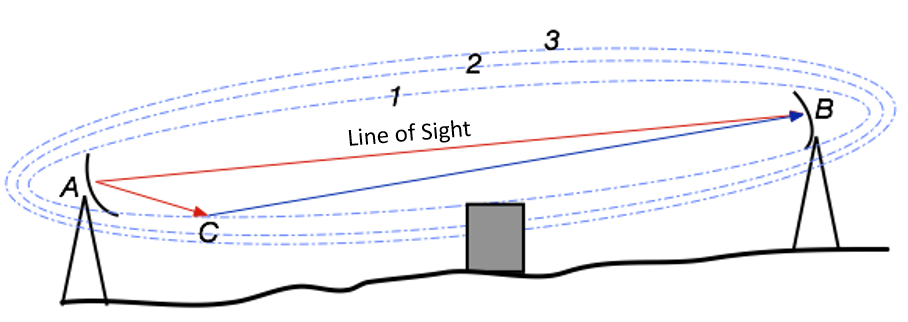
\includegraphics[scale=0.65]{figures/fresnel_zones.png}
	\caption{Fresnel zones between transmitter and receiver}
	\label{fig:3fresnel_zones}
\end{figure}

The figure above shows three examples of Fresnel zones, but there is an infinite number of them. The first zone is the one that has most effect on the performance of the Wireless Network. If there are any obstructions, such as buildings, trees or hills, in the first Fresnel zone, the signal will be affected by them and, consequently, would be weaker at the receiver.

Therefore, it is essential to keep the first Fresnel zone clear of obstruction when planning wireless links. However, it is impractical to avoid 100$\%$ of the obstructions in the real-life. Thus, based on (\hl{refhereimportant})27.maj 09:36, at least 60 $\%$ of the signal should be clear of obstructions. However, to get optimum performance it is recommended to keep the signal 20$\%$ or less blocked.

\subsection{Fresnel zone calculations}
The figure \ref{fig:fresnel_zones} represents the first Fresnel zone between the antennas on the buildings A and B. The radius \textit{r} corresponds to the radius of the Fresnel zone at the point P. 

\begin{figure}[H]
	\centering
	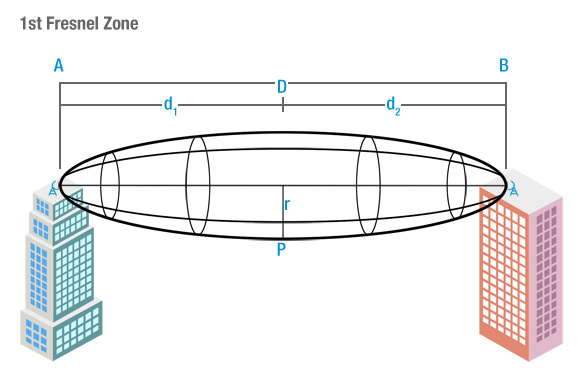
\includegraphics[scale=0.70]{figures/fresnel_zone.jpg}
	\caption{Fresnel zones}
	\label{fig:fresnel_zones}
\end{figure} 

Using the equation \ref{fresnel_zone_cal}, it is possible to calculate the radius, $r_n$, of the nth Fresnel zone at any point P, depending on the wavelength of the transmitted signal, $\lambda$. Thus, $d_1$ and $d_2$ represent the distances between the point P and the antennas A and B, respectively, in figure \ref{fig:fresnel_zones}.

\begin{align}
r_n = \sqrt{\frac{n \lambda d_1 d_2}{d_1+d_2}} \label{fresnel_zone_cal}
\end{align}

On the other hand, it is often useful to know the maximum radius of the zone. The radius of the Fresnel zone achieves its maximum when both distances $d_1$ and $d_2$ have the same size ($d_1=d_2$, which means that $d_1+d_2=D$). Based on the relation between the wavelength and the frequency, $\lambda = \frac{c}{f}$, and on the equation \ref{fresnel_zone_cal}, the radius of the first Fresnel zone can be calculated using the equation \ref{eq:fresnel_radius3}. In this equation, the frequency, $f$, is in gigahertz, and the total distance, $D$, is in kilometres in order to calculate the radius, $r$, in metres.

\begin{align}
r_1 = \sqrt{\frac{c}{f}\frac{d_1 d_2}{d_1+d_2}} = \sqrt{\frac{c}{f}\frac{d^2}{2d}}, d_1=d_2=d \label{eq:fresnel_radius1}
\end{align}

\begin{align}
r_1 = \sqrt{\frac{c}{2}}\sqrt{\frac{d}{f}} = \sqrt{\frac{c}{4}}\sqrt{\frac{D}{f}}, d=\frac{D}{2} \label{eq:fresnel_radius2}
\end{align}

\begin{align}
r_1 = 8.657 \sqrt{\frac{D}{f}} \label{eq:fresnel_radius3}
\end{align}

\subsection{Fresnel Zones examples without curvature of the earth}
In equation \ref{eq:fresnel_radius3}, by changing the distance between the antennas, $D$, it is clear that the radius, $r$, of the Fresnel zone will also change. In this subsection, there are three examples and some parameters are changed in order to analyse the behaviour of the radius' size. In the following examples, a frequency of 2.4 Ghz is used but the curvature of the earth is not considered. 

The first example shows an antenna and a UA at a height of 20 and 100 meters, respectively, and the distance between them is 10km.

\begin{figure}[H]
	\centering
	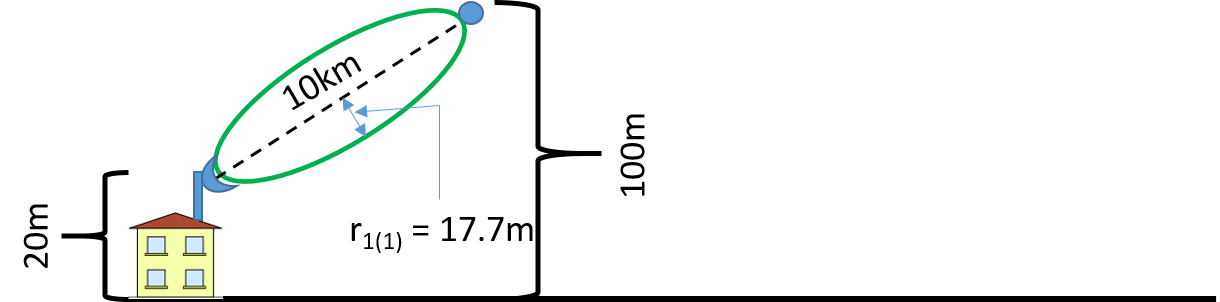
\includegraphics[scale=0.50]{figures/fresnel_10km.png}
	\caption{Fresnel zone when the distance between the transmitter and the receiver is 10km}
	\label{fig:fresnel_zones_10km}
\end{figure}  

In this first example, the radius is:
\begin{align*}
r_1 = 8.657 \sqrt{\frac{10}{2.4}} = 17.7m
\end{align*}

In the second example, the antenna and the UA keep at the same height as before but the distance between them is 20km.

\begin{figure}[H]
	\centering
	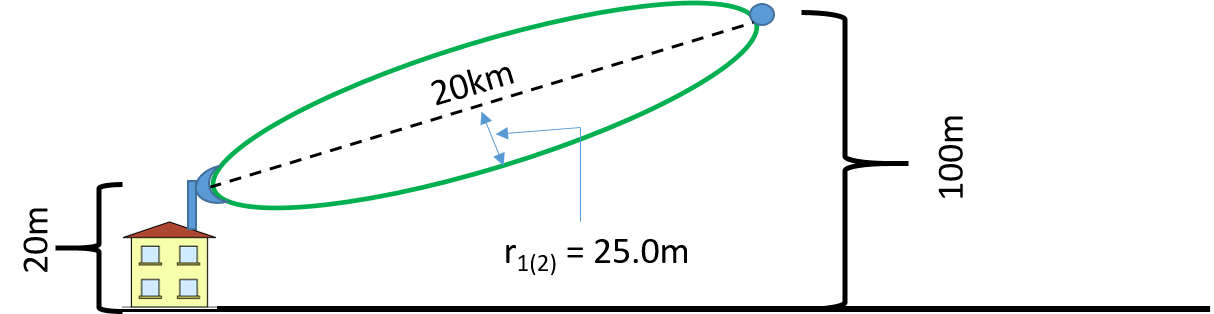
\includegraphics[scale=0.50]{figures/fresnel_20km.png}
	\caption{Fresnel zone when the distance between the transmitter and the receiver is 20km}
	\label{fig:fresnel_zones_20km}
\end{figure}  

The calculated radius is:
\begin{align*}
r_1 = 8.657 \sqrt{\frac{20}{2.4}} = 25.0m
\end{align*}

In the last example of this subsection, the antenna and the UA keep at the same height as in the previous examples but the distance between them is 50km.

\begin{figure}[H]
	\centering
	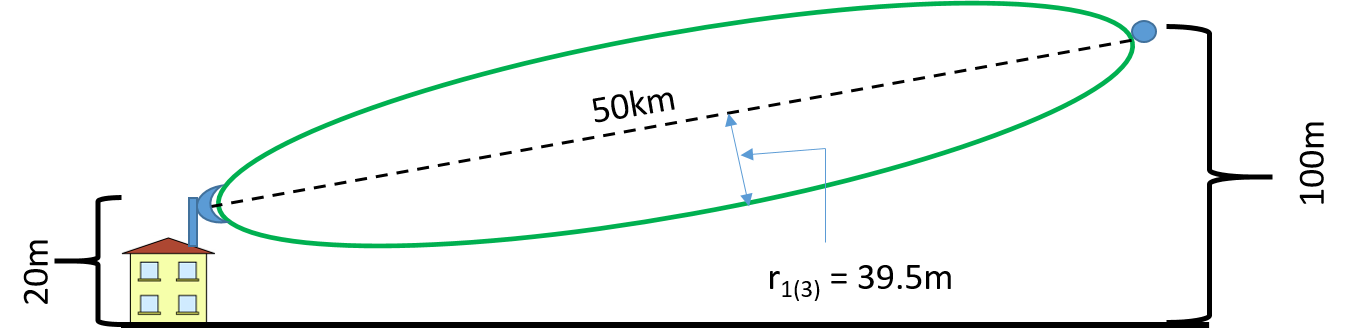
\includegraphics[scale=0.50]{figures/fresnel_50km.png}
	\caption{Fresnel zone when the distance between the transmitter and the receiver is 50km}
	\label{fig:fresnel_zones_50km}
\end{figure}  

In the last case, the calculated radius is:
\begin{align*}
r_1 = 8.657\sqrt{\frac{50}{2.4}} = 39.5m
\end{align*}

In these examples it is demonstrated that the radius of the Fresnel zone increases when the distance between the antennas increases.

\subsection{60$\%$ Clearance Zone of the first Fresnel zone}
As was described in the beginning of this section, it is difficult to have a first Fresnel zone without any obstructions. However, a percentage of obstruction equal or smaller than 40$\%$ makes the connection possible between the transmitter and the receiver.

In this subsection, some examples will demonstrate how tall a structure can be at the center of the first Fresnel zone, taking into account the 60$\%$ clearance. In order to be able to do the calculations the equation \ref{eq:60_percent_radius} was used.

\begin{align}
r_1 = 8.657\sqrt{\frac{0.6D}{f}}\label{eq:60_percent_radius}
\end{align}

For an ideal case, assuming that both antennas are at a height of 20 meters (operating at 2.6GHz) and the distance between them is 10km, the radius is given by the equation \ref{eq:100_distance10}.

\begin{align}
r_1 = 8.657\sqrt{\frac{10}{2.4}} = 17.7m\label{eq:100_distance10}
\end{align}

In this case, the first Fresnel zone would pass just 2.3 meters above the ground level in the middle of the link. 

\begin{figure}[H]
	\centering
	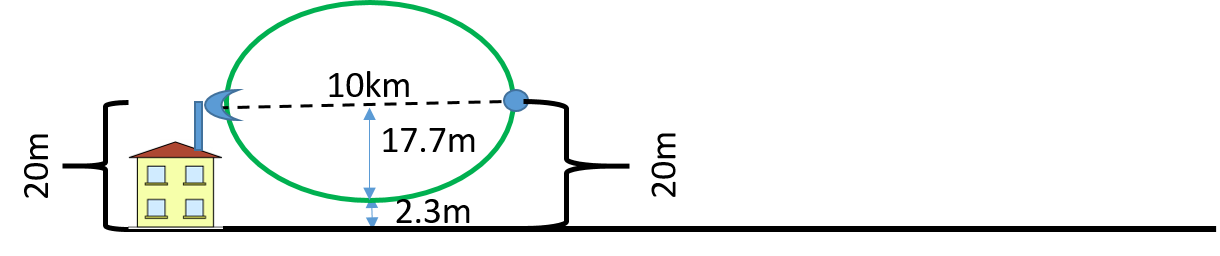
\includegraphics[scale=0.50]{figures/fresnel_10km_height.png}
	\caption{Fresnel zone when the antennas have the same height (20 meters) and when the distance between them is 10km.}
	\label{fig:fresnel_zones_10km_height}
\end{figure}  

In order to calculate how tall a structure should be, it is necessary to calculate the radius of the Fresnel zone when the signal is 60$\%$ cleared (equation \ref{eq:60_distance10}).

\begin{align}
r_{1(60\%)} = 8.657\sqrt{0.6 \frac{10}{2.4}} = 13.7m\label{eq:60_distance10}
\end{align}
  
Therefore, knowing that the height of the longitudinal axis of the ellipsoid is the same as the one of both antennas, it is possible to calculate the maximum altitude of the obstruction. This altitude can be obtained by subtracting the antenna height with the radius calculated in equation \ref{eq:60_distance10}.

\begin{align}
\text{Maximum Obstruction Height} = 20 - 13.7 = 6.3m\label{eq:height_obstruction}
\end{align}

Hence, for this specific example, the maximum tolerated height of any obstruction located in the middle point between both antennas is 6.3m. An illustration of this situation is shown in figure \ref{fig:fresnel_zones_10km_60procent}.

\begin{figure}[H]
	\centering
	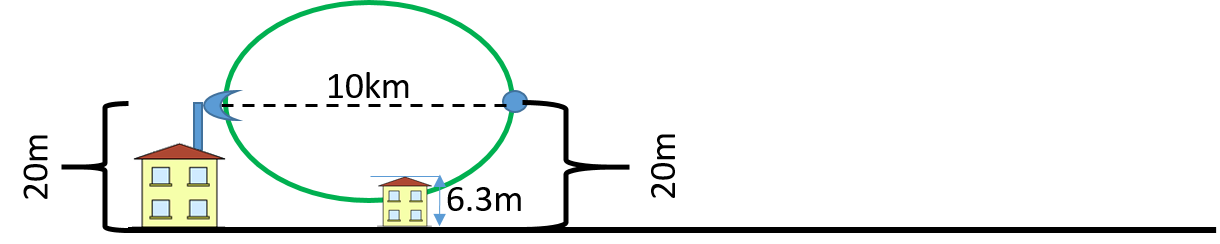
\includegraphics[scale=0.50]{figures/fresnel_10km_60procent.png}
	\caption{Fresnel zone with a 40$\%$ of the signal is blocked.}
	\label{fig:fresnel_zones_10km_60procent}
\end{figure}  

An obstruction higher than 6.3m will give less than 60$\%$ clearance of the Fresnel zone. To prevent this problem, the antenna need to be positioned higher up, the frequency could be changed or the direction of the link should be changed to avoid obstacles.

\subsection{Fresnel zones examples with curvature of the earth}
For longer distance links the curvature of the earth comes into play and may become an obstruction into the Fresnel zone, causing signal losses. Moreover, the longer the distance between the antennas, the greater the radius of the Fresnel zones. Equation \ref{eartheffect} allows to calculate the height difference of Earth's Curvature, $H$, at the mid-point between the two antennas. In order to do the previous calculation, it is necessary to include one parameter related to the total distance between both antennas, $D$ (km), and one related to the effective radius of Earth, $E_r = 8 504 km$.

Furthermore, figure \ref{fig:fresnel_50km_curvature} is an illustration where the curvature of the earth is taking into account. On this figure the antennas on the building and the UA are at 77m height and the distance between them is 50km. 

\begin{align}
H = \frac{1000\cdot D^2}{8\cdot E_r}\label{eartheffect}
\end{align}

\begin{figure}[H]
	\centering
	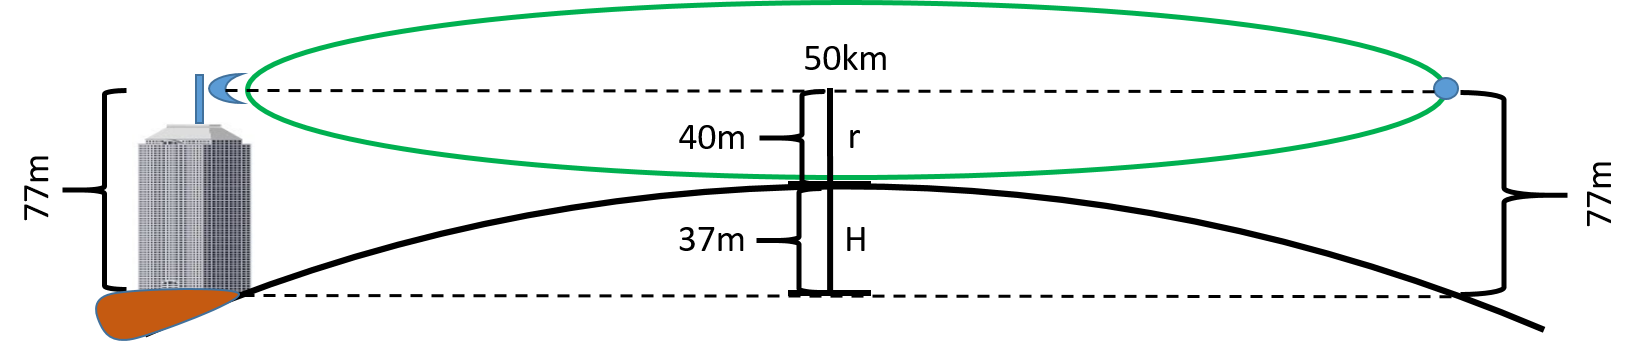
\includegraphics[scale=0.50]{figures/fresnel_50km_curvature.png}
	\caption{Fresnel zone in 50km distance with curvature of the earth taken into account.}
	\label{fig:fresnel_50km_curvature}
\end{figure}

Based on equation \ref{eartheffect}, the height difference of the earth's curvature at the mid-point between the UA and the building:
\begin{align}
\text{H} = \frac{1000 D^2}{8 \cdot E_r} = \frac{1000 \cdot 50^2}{8\cdot 8504} = 36.7m \approx 37m 
\end{align}

Furthermore, the radius of the first Fresnel zone:
\begin{align*}
\text{r} = 8.657\cdot \frac{0.6\cdot D}{f} = 8.657\cdot \frac{50}{2.4} = 39.5m \approx 40m 
\end{align*}

On the other hand, the maximum height of the obstruction between the two devices within the 60$\%$ clearance zone can be calculated with the equations \ref{radius_60}, \ref{Obs_max_height} and \ref{height_max_with_curv}. These calculations are illustrated on figure \ref{fig:fresnel_50km_curvature_obstacle}.

\begin{align}
r_{1(60\%)} &= 8.657\cdot \frac{0.6\cdot D}{f} = 8.657\cdot \frac{0.6\cdot 50}{2.4} = 30.6m \approx 31m \label{radius_60}
\end{align}

The maximum height of the obstruction with the curvature of the earth included:
\begin{align}
\text{Obs}_{\text{max height}} &= 77m - r_{1(60\%)} = 77m - 31m = 46m \label{Obs_max_height}
\end{align}

The actual maximum height of the obstruction:
\begin{align}
\text{height}_{\text{max with curv}} &= \text{Obs}_{\text{max height}} - H = 46m - 37m = 9m\label{height_max_with_curv}
\end{align}

\begin{figure}[H]
	\centering
	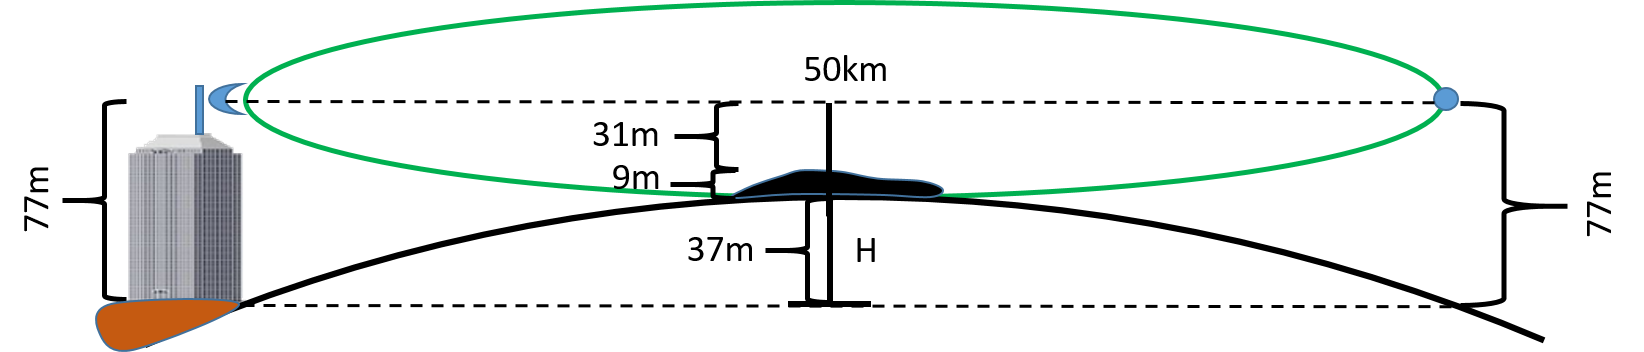
\includegraphics[scale=0.50]{figures/fresnel_50km_curvature_obstacle.png}
	\caption{Fresnel zone taking into account the curvature of the earth and the 60$\%$ clearance.}
	\label{fig:fresnel_50km_curvature_obstacle}
\end{figure}  

Figure \ref{fig:fresnel_50km_curvature_obstacle} shows that it's important to consider the curvature of the earth. Here the obstruction can only be at the height of 9m, since the curvature is an obstruction itself and takes 37m. However, it is important to note that this example only implies when the longitudinal axis of the ellipsoid is the same as the one of both antennas. But nonetheless it gives a good understanding that the Fresnel zones are important factors when building a wireless link network.

% \section{Telemetry}\label{sec:telemetry}
One of the main goal of drone surveillance is to procure relevant data. This is done by means of telemetry which is an automated communication process. In this process the data collected is transmitted to a receiving equipment for further processing and monitoring. 

!!! ADD MORE INFO !!!

!!! ADD FIGURE !!!

!!! HOW WE USE IT ? !!!
\section{MAVLink Protocol}\label{sec:mavlink}
Taking the application at hand, inter-communication between systems is required such that transmission of aircraft parameters (e.g. location, heading angle and speed) to the ground station is fulfilled. In some cases, the whole system will operate in a low communication scenario in such a way that a low bandwidth allocation is essential. In this sense, given its characteristics a favorable candidate for the UAS would be the Micro Air Vehicle Link (MAVLink) protocol.

\subsection{Packet Structure}
In digital communication the information is sent through packets, in this case the data are the UAS parameters. Thus, for further understanding the packet structure of the MAVLink protocol can be as seen in Table \ref{tab:mavlink}.

\begin{table}[H]
	\centerline{
	\begin{tabular}{|c||c|c|}
		\hline
		Field name       & Index (Bytes)  & Purpose											     \\ \hline\hline
		Start-of-frame   &      0         & Start of frame transmission 							   \\ \hline
		Pay-load-length  &      1         & Length of payload (n)       							   \\ \hline
		Packet sequence  &      2    	  & Sent sequence counter (detect packet loss)                 \\ \hline
		System ID        & 		3		  & Sending system identification 							   \\ \hline
		Component ID     & 		4 		  & Sending component identification 						   \\ \hline
		Message ID       & 		5 		  & Message identification (correctly decoded)      		   \\ \hline
		Payload          &   6 to (n+6)   & Data into the message, depends on Message ID        	   \\ \hline
		CRC              & (n+7) to (n+8) & Check-sum of packet (excluding packet start sign)          \\ \hline
	\end{tabular}}
	\caption{MAVLink packet structure}
	\label{tab:mavlink}
\end{table}

The CRC field ensures message integrity of each packet. Another function of the CRC is to establish that both sender and receiver agree on the message transfer.

\subsection{Messages}
As stated above the payload from the packets are MAVLink messages. Also, every message can be identified by its ID field on the packet. Additionally, an XML document (in MAVLink source) has the definition of all the data stored on that payload. A sample of such an XML document can be seen in Figure \ref{fig:mav_msg} which describes a message with a 24 number ID giving GPS relevant information. Thus, from this message it can be observed the latitude, longitude and altitude in the WGS84 coordinate system.

\begin{figure}[H]
	\centering
	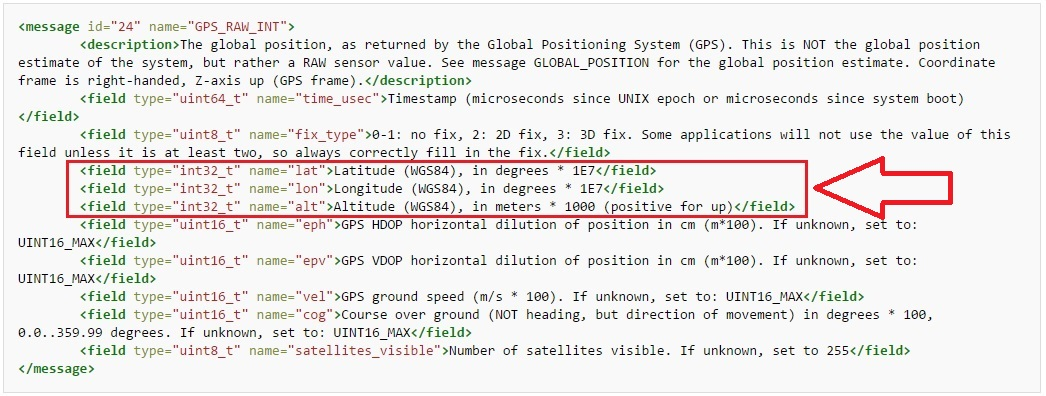
\includegraphics[scale=0.5]{figures/mavlink_msg.jpg}
	\caption{Example of a MAVLink message XML document}
	\label{fig:mav_msg}
\end{figure}

To be noted that the XML document describes the logical ordering of the fields for the protocol, not the actual wire format.

\subsection{Advantages}
To sum up, taking into account the advantages of the MAVLink protocol it can be said that it is a viable option in the case of the UAS at hand:
\begin{itemize}
	\item Small packet size
	\item Message verification
	\item Low bandwidth allocation
	\item Useful at low communication scenario
\end{itemize}


\chapter{Modelling}\label{ch:model}

!!! INTRO !!!

??? State-space model ???


<<<<<<< HEAD
e\section{Moving angle system}\label{servo_model}
=======
\section{DC Servomotor}\label{sec:servo_model}
>>>>>>> fe5f2cb36f351516ba58e4a6b413d6fdce8806bc

The use of a tracking antenna system requires a device to change the orientation of the antennas. The moving angle system is performing this task and is composed of a DC servomotor for the rotational movement of the antennas, a gear to have a precise change of the angles, and a sensor to keep track of the actual angle and compare it to the reference.

The DC servomotor, presented in the section \ref{sec:servo_motor}, can be divided in two different groups: the DC motor and the servomechanism.

DC motor is an actuator which converts electrical energy to mechanical rotation. In the figure \ref{dcmotor_circuit} it is possible to see the model of this motor. DC motors are a type of motors which were built to receive a voltage as an input and, after converting this voltage, to apply a specific velocity on its shaft. In other words, DC motors are able to control the velocity of the shaft.

\begin{figure}[H]
\centering
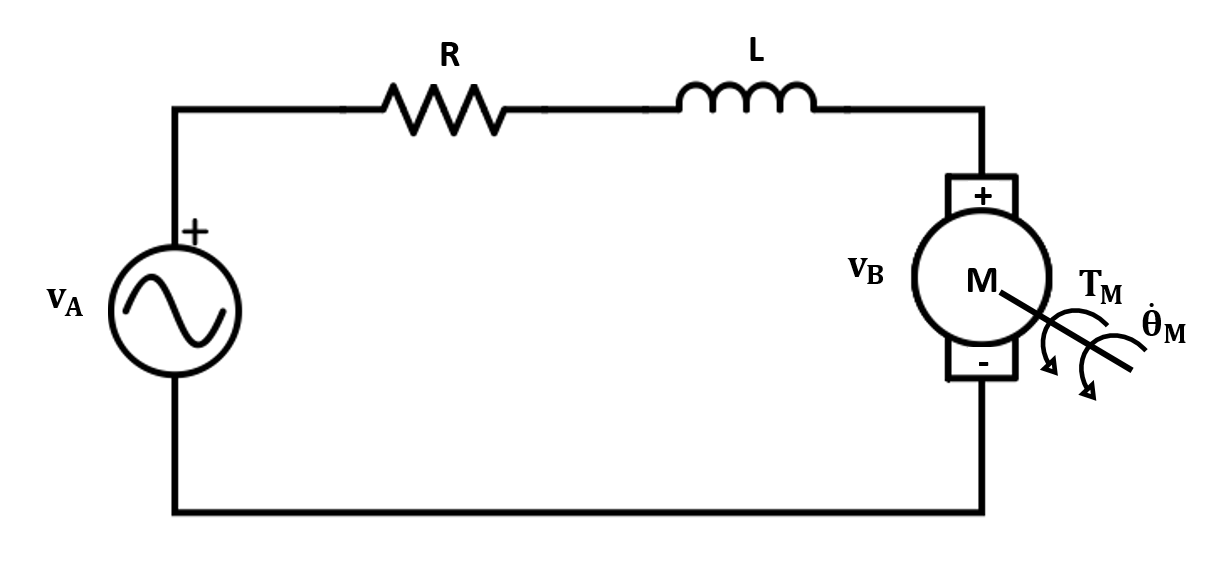
\includegraphics[scale=0.5]{figures/dcmotor_circuit.png}
\caption{Circuit of the DC motor}
\label{dcmotor_circuit}
\end{figure}

The circuit of the previous figure is described by the equations \ref{DC_motor_equation1}, \ref{DC_motor_equation2} and \ref{DC_motor_equation3}. It is possible to observe that between the source unit and the motor there are two elements (resistance and inductance). These elements are important due to the fact that they are the responsible for the stability of the system, avoiding a motor overload. Hence, the relation between the current and the difference between the voltage of the source and the one of the motor is made through an admitance.

\begin{equation}\label{DC_motor_equation1}
v_{a}= v_{b}+i_{a} R_{a}+L_{a}\frac{\mathrm{d} i_{a}}{\mathrm{d} t}
\end{equation}

\begin{equation}\label{DC_motor_equation2}
V_{a}(s)= V_{b}(s)+I_{a}(s) R_{a}+sL_{a}I_{a}(s)
\end{equation}

\begin{equation}\label{DC_motor_equation3}
I_{a}(s)= \frac{V_{a}(s)-V_{b}(s)}{R_{a}+sL_{a}} , I_{a}(s)= G_{I}(V_{a}(s)-V_{b}(s))
\end{equation}

The model of the figure \ref{model1} is the representation of the equation \ref{DC_motor_equation3}.

\begin{figure}[H]
\centering
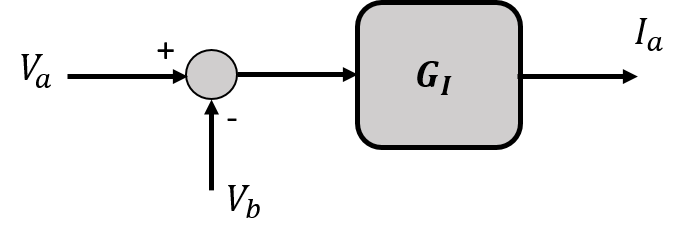
\includegraphics[scale=0.6]{figures/model1.png}
\caption{Relation between the input and the feedback voltage and the current of the circuit}
\label{model1}
\end{figure}

Furthermore, the sum of torques applied on the motor depends on the load attached to the motor shaft. The inertial and damping behaviours of the load can be represented as a inertia coefficient, $J_{e}$, and a viscous damping coefficient, $D_{e}$. This total tendency of a force to rotate an object about an axis is represented by $T_{m}$ which is described through the equation \ref{torque_time}. 

\begin{equation}\label{torque_time}
T_{m}(t)= J_{e}\frac{\mathrm{d} \dot{\theta}_{m}(t)}{\mathrm{d} t}+D_{e}\dot{\theta}_{m}(t)
\end{equation}

However, the servomotor is a type of motor which is able to control the position of the shaft. Using a potentiometer it is possible to send an electrical signal with the information about the angle. Thus, using the relation between the velocity and the position described in the equation \ref{theta_relation}, it is possible to write the equation \ref{torque_frequency_theta}.

\begin{equation}\label{theta_relation}
\dot{\theta}_{m}(s)= s\theta_{m}(s)
\end{equation}

\begin{equation}\label{torque_frequency_theta}
T_{m}(s)= (s^{2}J_{e} + sD_{e})\theta_{m}(s)
\end{equation}

The torque is also proportional to the current that passes through the circuit. The constant of proportionality is called torque constant and the relation between the torque and the current is presented in the equations \ref{torque_curr1} and \ref{torque_curr2}.

\begin{equation}\label{torque_curr1}
T_{m}(t)= K_{t} i_{a}(t)
\end{equation}

\begin{equation}\label{torque_curr2}
T_{m}(s)= K_{t} I_{a}(s)
\end{equation}

Based on the previous equations and on the model in the figure \ref{model1} it is possible to build the model in the figure \ref{model2}.

\begin{figure}[H]
\centering
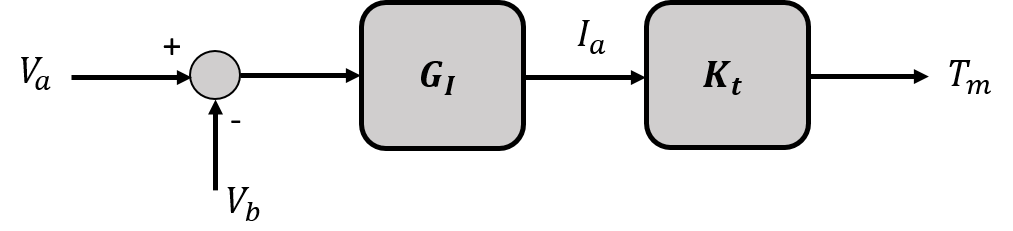
\includegraphics[scale=0.6]{figures/model2.png}
\caption{Relation between the voltage and the applied torque}
\label{model2}
\end{figure}

The applied torque $T_{m}(s)$ described in the previous equations can be also related to the angle position $\theta_{m}(s)$ through the equations \ref{torque_frequency} and \ref{torque_frequency_G}.

\begin{equation}\label{torque_frequency}
T_{m}(s) I_{a}(s)= (s^{2}J_{e} + sD_{e})\theta_{m}(s)
\end{equation}

\begin{equation}\label{torque_frequency_G}
\theta_{m}(s)= G_{\theta}(s)\times T_{m}(s) , G_{\theta}(s)=\frac{1}{s^{2}J_{e} + sD_{e}}
\end{equation}

\begin{figure}[H]
\centering
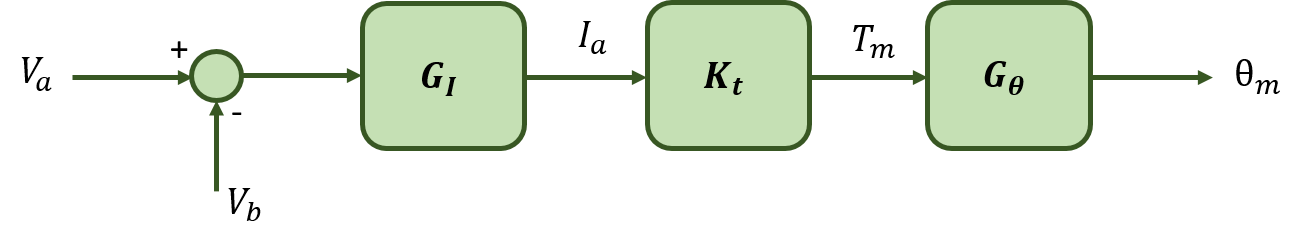
\includegraphics[scale=0.6]{figures/model3.png}
\caption{Relation between the voltage and the angle of the shaft}
\label{model3}
\end{figure}

Finally, it is also possible to calculate the relation between the output theta and voltage. Thus, the comparison between the output and the input voltage allows the formation of a closed loop using a feedback (figure \ref{model4}).

\begin{equation}\label{feedback1}
v_{b}(t)= K_{b}\frac{\mathrm{d} \theta_{m}(t)}{\mathrm{d} t}
\end{equation}

\begin{equation}\label{feedback2}
V_{b}(s)= sK_{b}\theta_{m}(s)
\end{equation}

\begin{figure}[H]
\centering
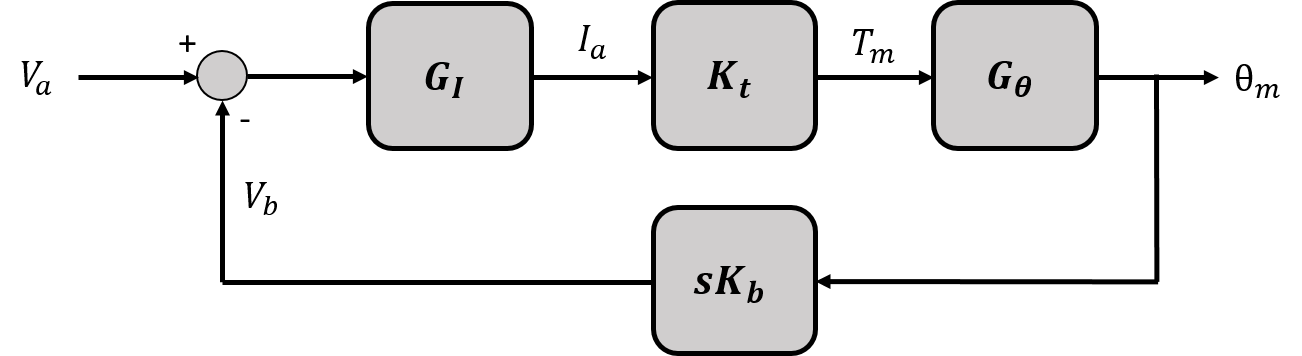
\includegraphics[scale=0.6]{figures/model4.png}
\caption{Model of a servomotor}
\label{model4}
\end{figure}

A gear was added to the servomotor to reduce its speed and obtain a better precision for the output angle. Time to reach the desired angle and required precision were taken into account to choose a gear ratio.
For instance, a gear ratio of 0.001 means that 1000 rotations of the motor will result in a single rotation at the end of the system.

\begin{figure}[H]
\centering
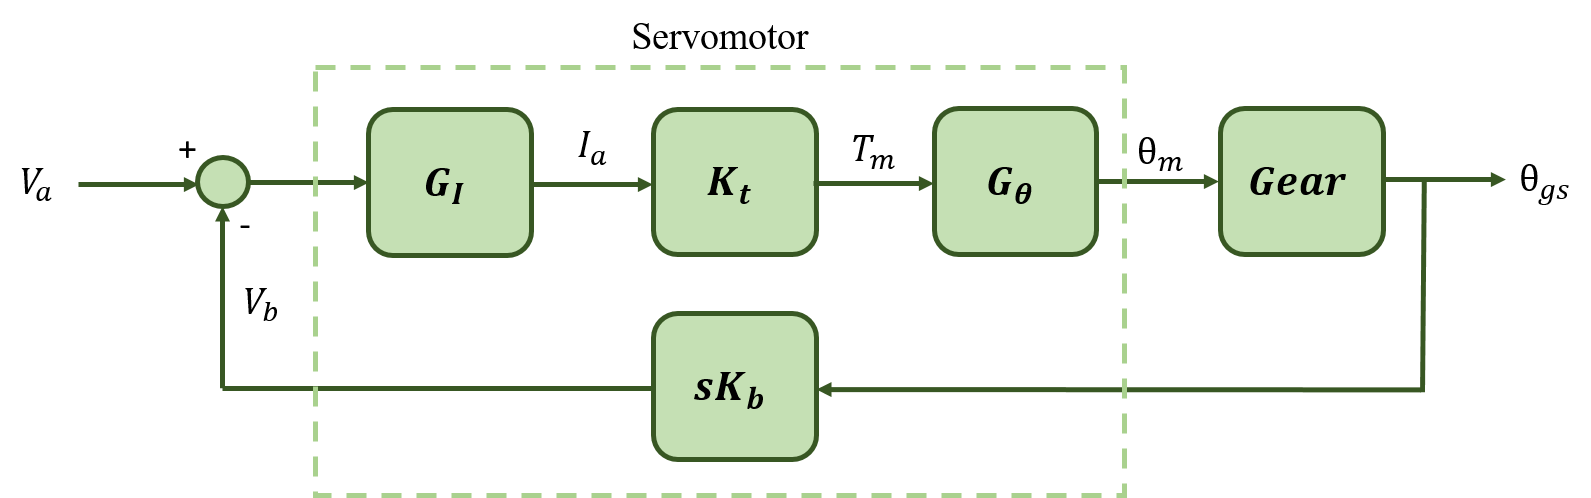
\includegraphics[scale=0.6]{figures/servo+gear.png}
\caption{Servomotor with a gear}
\label{model4}
\end{figure}

In order to control the antennas, the input of the system is the desired angle. However, the servomotor requires an electrical signal input (voltage) that represents the rotations needed. This voltage is the output of a controller whose input is a comparison between the reference angle and the actual one (error angle). The current angle of the system is given by a sensor.
Assuming that the sensor is not ideal, the disturbances caused by it can be simulated by adding a white noise to the feedback of the plant.

\begin{figure}[H]
\centering
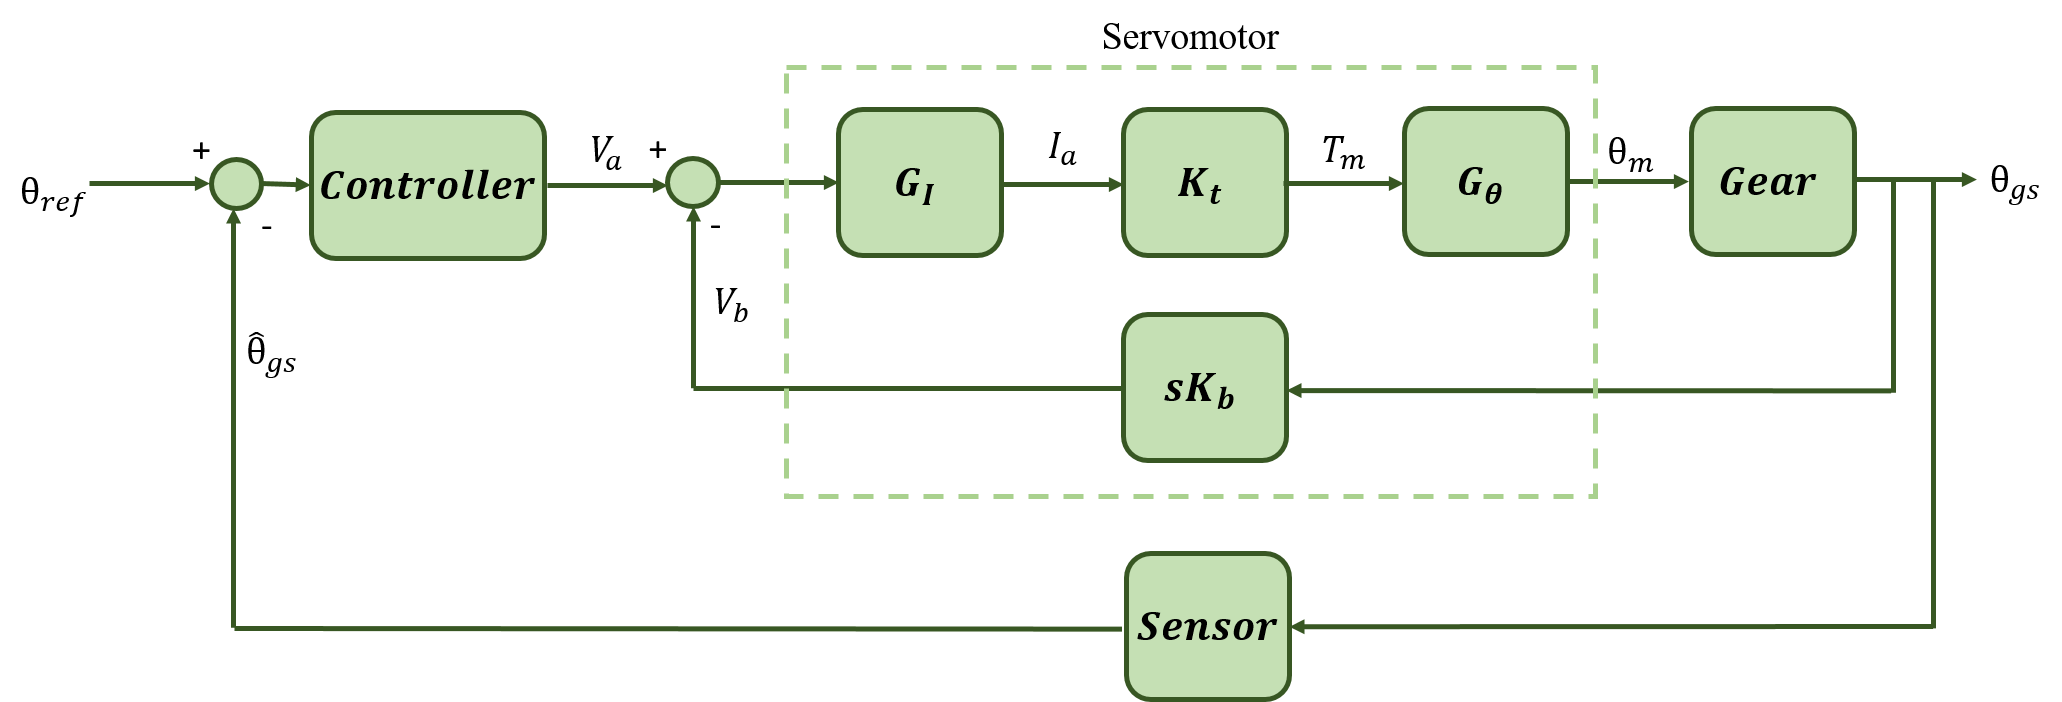
\includegraphics[scale=0.5]{figures/servo+gear+noise.png}
\caption{Limitation of the voltage into the servomotor and its gear}
\label{model4}
\end{figure}

High voltage value can be the consequence of the controller trying to reach the desired value in the fastest way. With a view to procure a range of voltage that the motor can handle and prevent any damage, a saturation box was included.

\begin{figure}[H]
\centering
\includegraphics[scale=0.4]{figures/complete_model.png}
\caption{Model of the Moving Angle System}
\label{model4}
\end{figure}


\section{Optimal Angle}\label{sec:opt_angle}
The right part of the Figure \ref{fig:2d_system} shows two PD controllers where each of them have a servomotor connected. The PD controller is explained in Section \ref{sec:pd_controller} and the servomotor is explained in Section \ref{sec:servo_model}. The left block have two output which is $\theta\_opt\_d$ and $\theta\_opt\_gs$. They are the optimal angle that the drone and ground station need to have to be pointing at each other (Figure \ref{fig:drone_gs}). The PD controllers purpose is to make the servomotors rotate the antenna to the correct position. The PD controllers take the error ($\theta\_opt\_d - \theta\_d$) for the drone and ($\theta\_opt\_gs - \theta\_gs$) for the ground station, and make the servomotors rotate the antenna to the correct position. When the error is zero, which means the input to the PD controller is zero, the antennas are at the correct angles.
\section{Antenna}\label{sec:antenna}

Based on the overview of the system made in Chapter \ref{ch:uas}, a modelling of the radiation pattern of the directional antenna is in due to be able to simulate the scenario.

The radiation patterns are a graphical way of representing the radiation properties of the antenna as a function of space. These patterns are very useful when it comes to how an antenna perform \cite{Balanis97}. As an example, Figure \ref{fig:radpattern} shows the radiation patterns of a real directional antenna.

\begin{figure}[H]
	\centerline{
	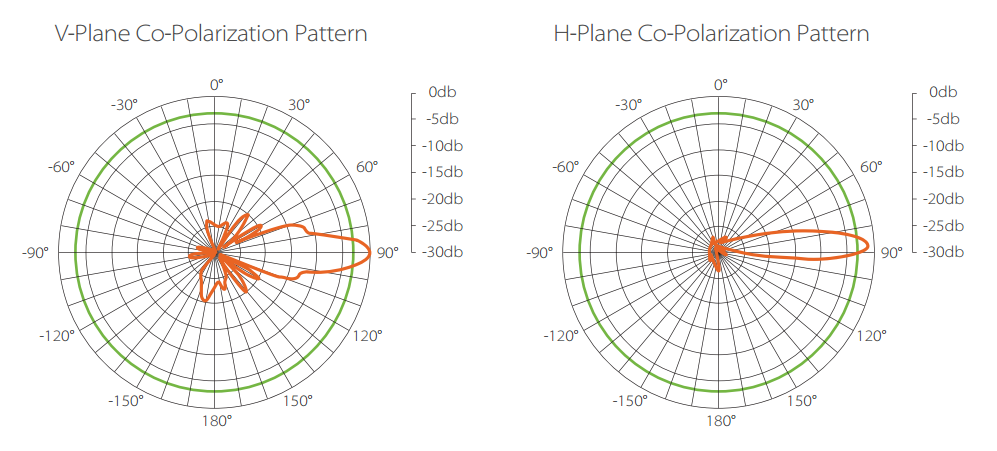
\includegraphics[scale=0.5]{figures/radpattern.png}}
	\caption{Radiation Pattern of a real directional antenna.}
	\label{fig:radpattern}
\end{figure}

\paragraph{}Note how, for a 3 dimensional radiation pattern, 2 planes are defined. These are the horizontal plane (H-plane) and the vertical plane (V-plane). For simplicity, during this project it is assumed that the radiation pattern is symmetric, and therefore, exactly the same for both planes.

\paragraph{}The concentric circles inside the plot represent the normalized power radiated in decibels (even though it is possible to find non-normalized plots as well). The closer to the center the circles are, the weaker the power gets in a logarithmic scale. 

\begin{table}[h]
	\centering
	\begin{tabular}{|c||c|c|}
		\hline
		Parameter & GS & UA\\ \hline\hline
		Type & Parabolic & Patch\\ \hline
		Polarization & Linear & Linear\\ \hline
		Frequency [GHz] & $2.4$ & $2.4$\\ \hline
		Gain [dB] & $24$ & $14$\\ \hline
		HPBW/$H(^{\circ})$ & $14$ & $45$\\ \hline
		HPBW/$V(^{\circ})$ & $10$ & $45$\\ \hline
	\end{tabular}
	\caption{Antennas specifications.}
	\label{table:1}
\end{table}

\paragraph{}Choosing the parabolic and the patch antennas showed in table \ref{table:1} a radiation pattern was build by using the mathematical function \textit{sinc}, as shown in Figure \ref{fig:sinc}.

\begin{figure}[H]
\hfill
\subfigure[Sinc function natural units.]{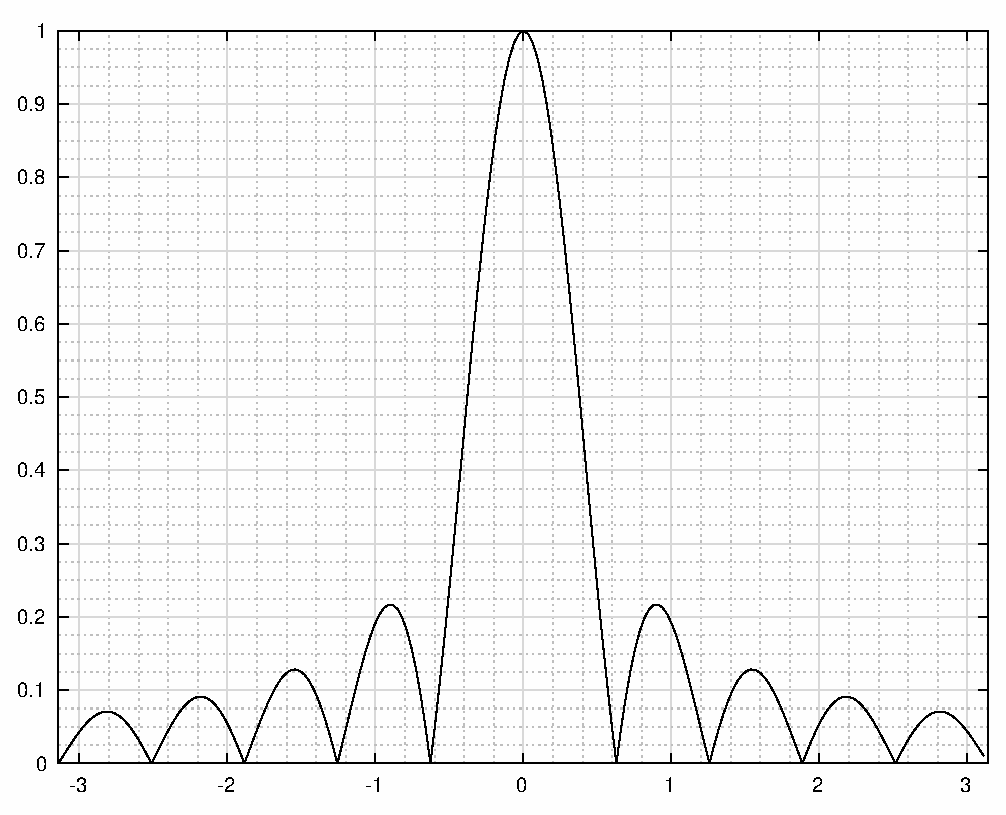
\includegraphics[width=0.45\textwidth]{figures/sinc1.eps}}
\hfill
\subfigure[Sinc function logarithmic units.]{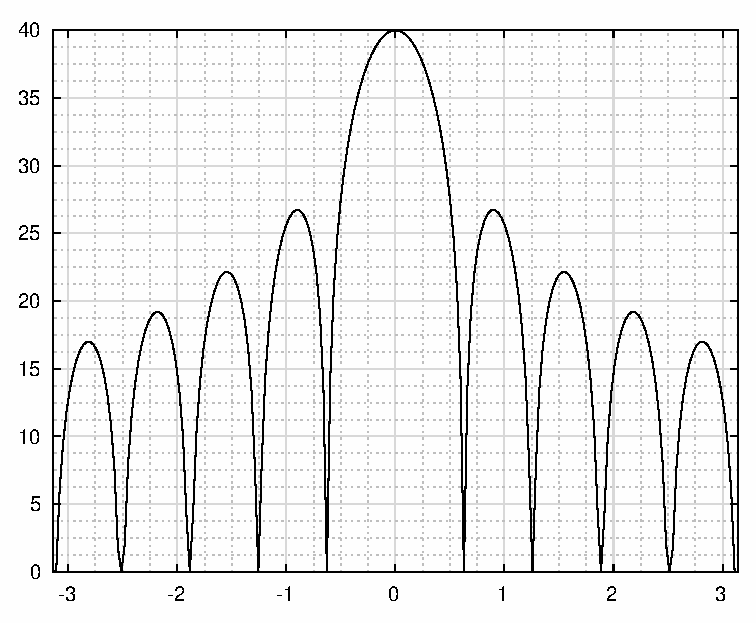
\includegraphics[width=0.45\textwidth]{figures/sinc2.eps}}
\hfill
\caption{Sinc function.}
\label{fig:sinc}
\end{figure}

Plotting this \textit{sinc} in a form of a radiation pattern, similar features of a real antenna can be achieved (Figure \ref{fig:radiationpattern}).

\begin{figure}[H]
	\centering
	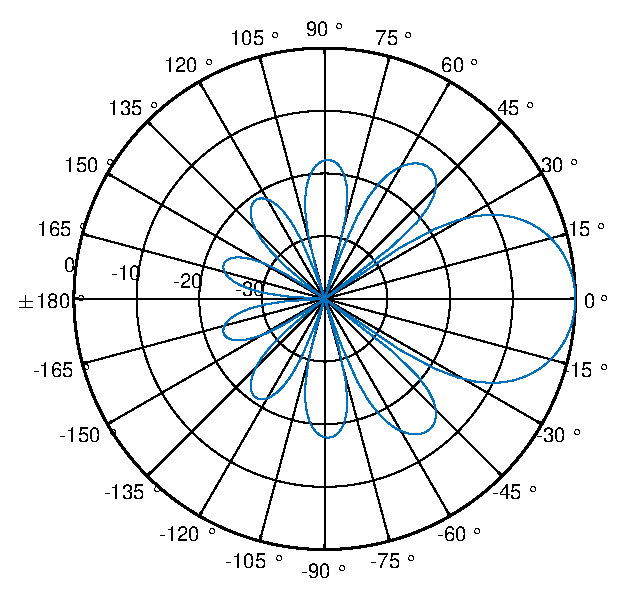
\includegraphics[scale=1.1]{figures/RadPattern.eps}
	\caption{Radiation Pattern based on sinc.}
	\label{fig:radiationpattern}
\end{figure}


%
%\begin{frame}{Controller}{}
%
%  \begin{block}{PID}
%
%  \end{block}
%  
%  \begin{block}{Tunning}
%
%  \end{block}
%
%  \begin{block}{Comparion}
%
%  \end{block}
%
%\end{frame}

%Overview
\begin{frame}{Modelling}{Moving Angle System}
  \begin{block}{Moving Angle System:}

	  \begin{itemize}
  	  	\item Servomotor
	  	\item Gear
	  	\item Sensor
	  	\item Controller
	  	\item Saturation
	  \end{itemize}

	  \begin{figure}
        \includegraphics[scale=0.24]{../report/figures/complete_model.png}
      \end{figure}
  
  \end{block}
\end{frame}


%Servomotor
\begin{frame}{Modelling}{Moving Angle System}
  \begin{block}{Moving Angle System:}

	  \begin{itemize}
	  	\item Servomotor - modelled
	  \end{itemize}

	  \begin{figure}
        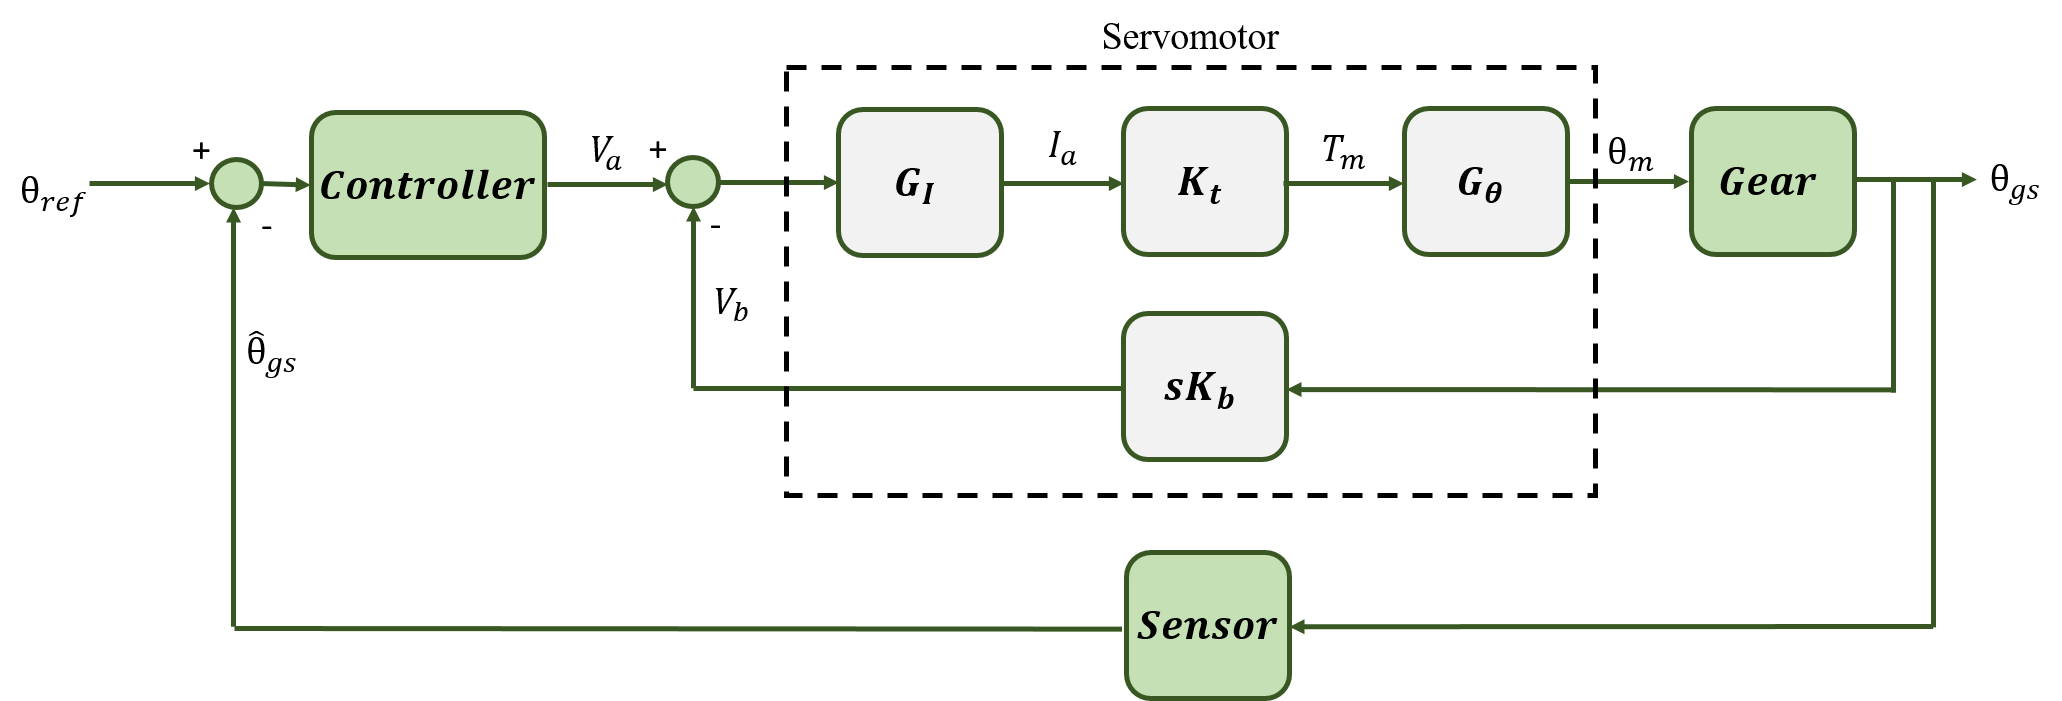
\includegraphics[scale=0.24]{../report/figures/servo+gear+noise+servomotor.png}
      \end{figure}
  
  \end{block}
\end{frame}

%Gear
\begin{frame}{Modelling}{Moving Angle System}
  \begin{block}{Moving Angle System:}
	  \begin{itemize}
	  	\item Gear - reduce speed and increase precision
	  \end{itemize}
	  \begin{figure}
        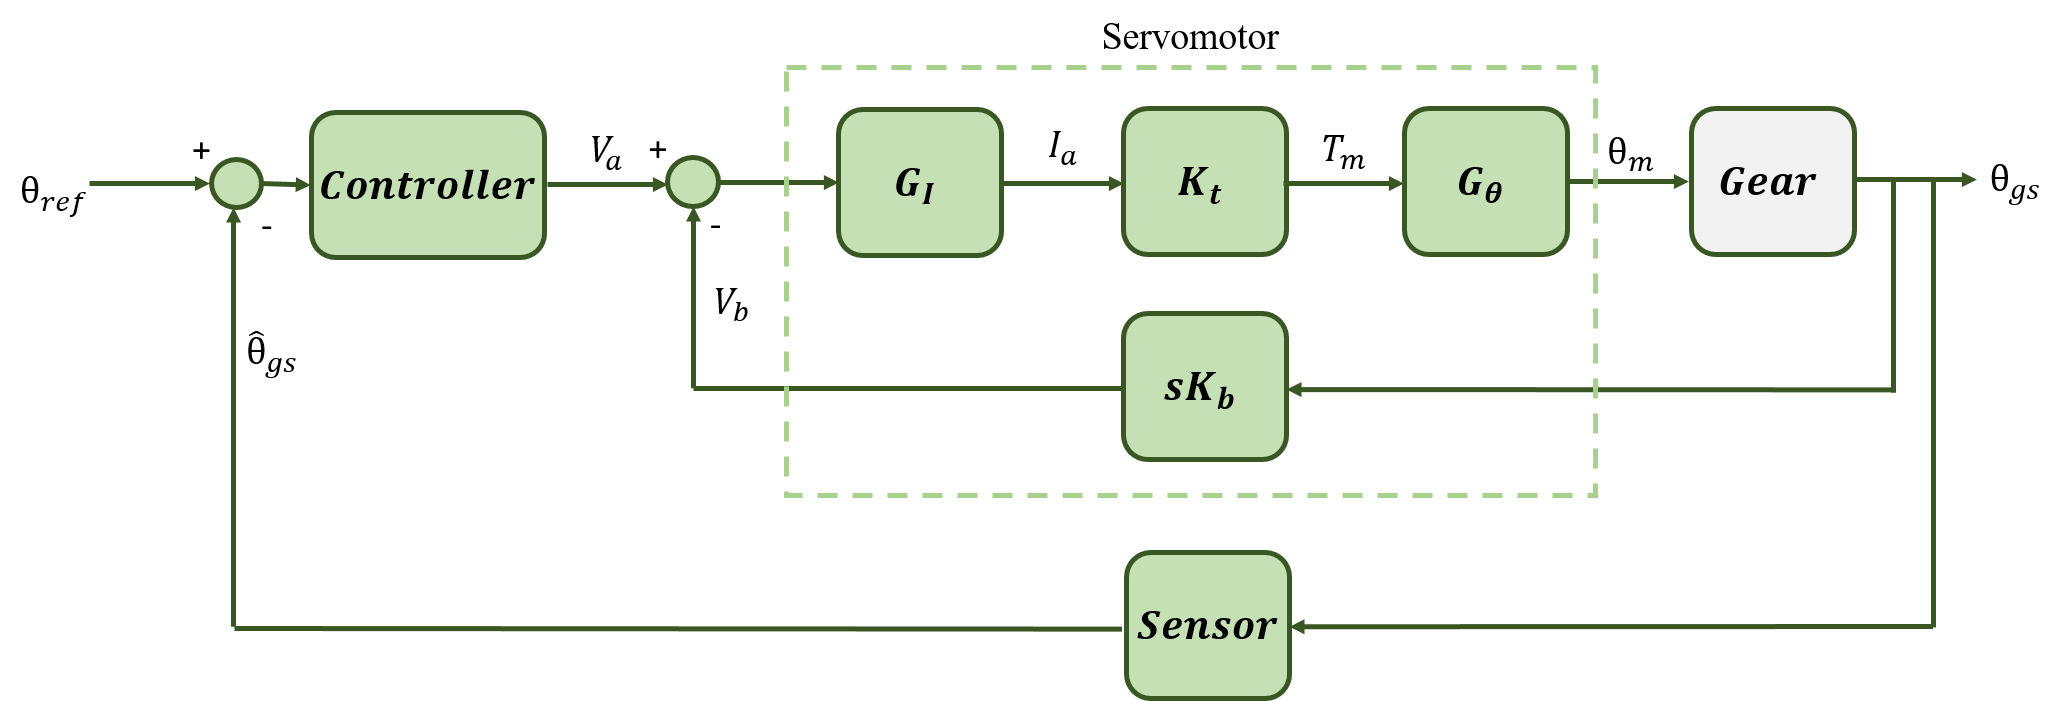
\includegraphics[scale=0.24]{../report/figures/servo+gear+noise+gear.png}
      \end{figure}  
  \end{block}
\end{frame}

%Sensor
\begin{frame}{Modelling}{Moving Angle System}
  \begin{block}{Moving Angle System:}

	  \begin{itemize}
	  	\item Sensor - measurement noise	  
	  \end{itemize}

	  \begin{figure}
        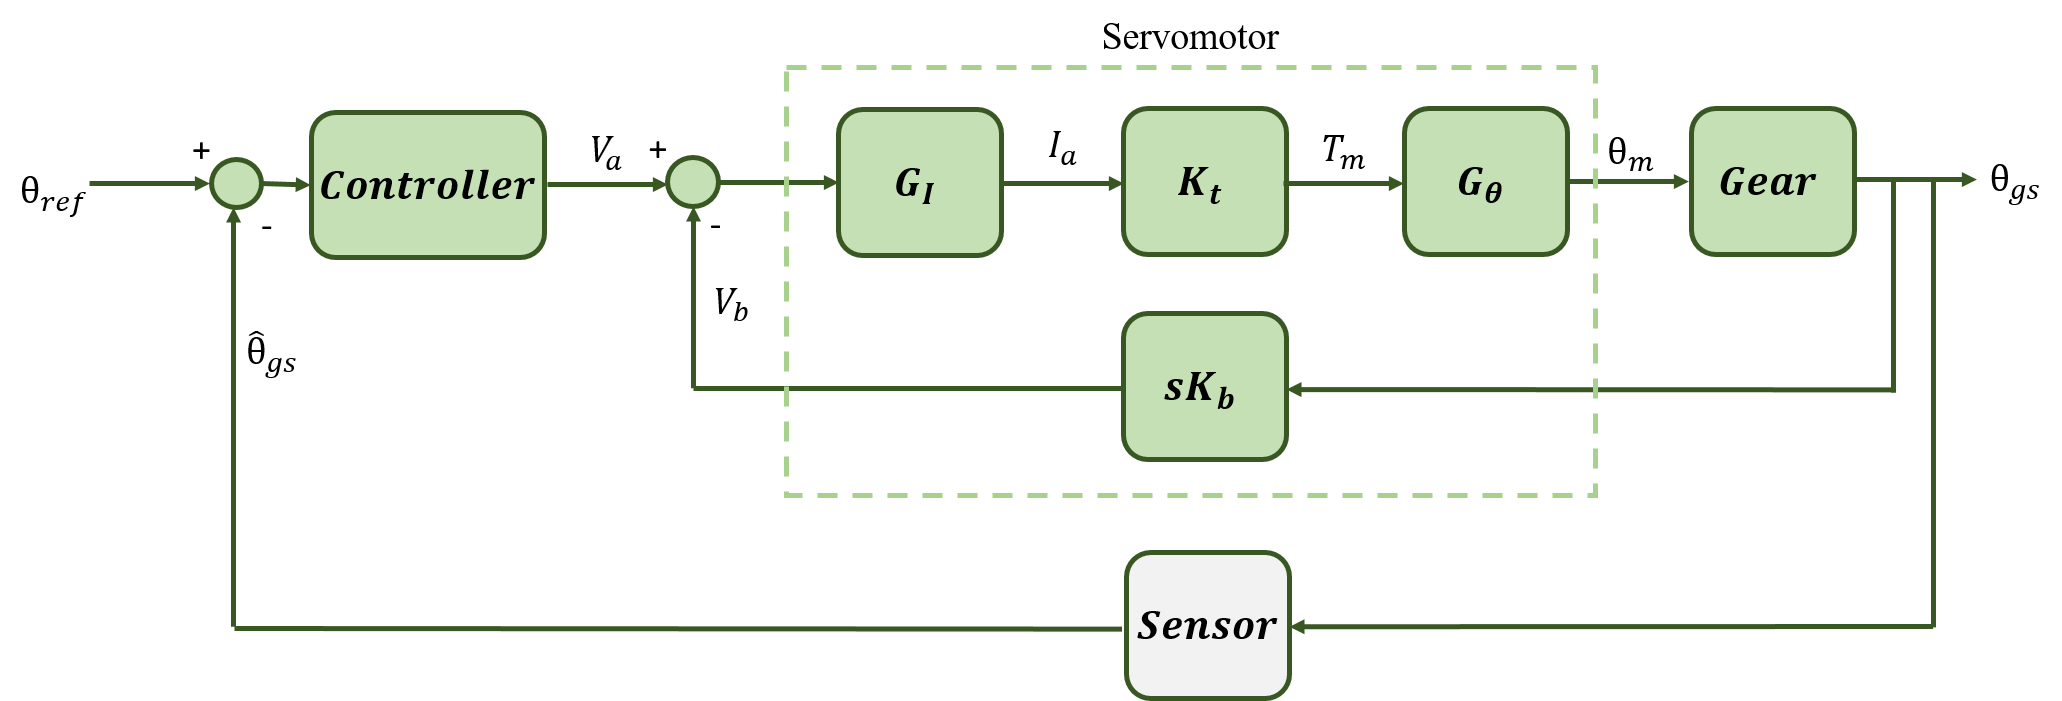
\includegraphics[scale=0.24]{../report/figures/servo+gear+noise+sensor.png}
      \end{figure}
  
  \end{block}
\end{frame}


%Controller
\begin{frame}{Modelling}{Moving Angle System}
  \begin{block}{Moving Angle System:}
	  \begin{itemize}
	  	\item Controller
	  \end{itemize}
	  \begin{figure}
        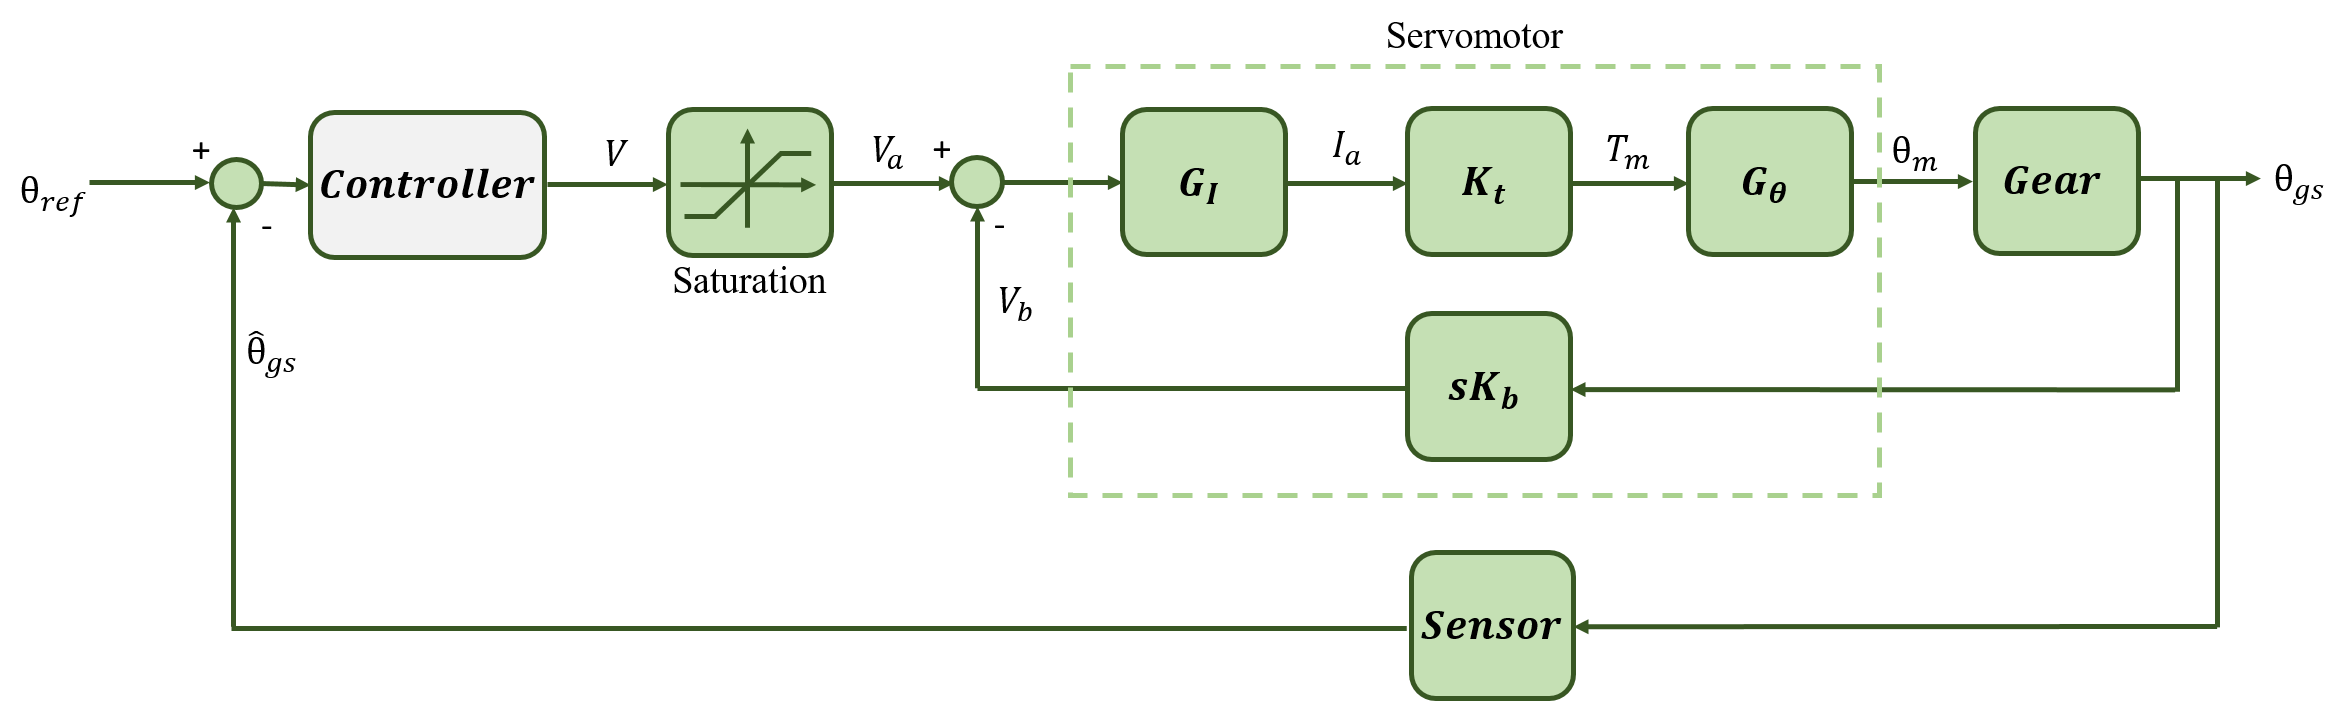
\includegraphics[scale=0.24]{../report/figures/servo+gear+noise+controller.png}
      \end{figure}
  \end{block}
\end{frame}

%Saturation
\begin{frame}{Modelling}{Moving Angle System}
  \begin{block}{Moving Angle System:}

	  \begin{itemize}
	  	\item Saturation - threshold set from -5V to 5V
	  \end{itemize}

	  \begin{figure}
        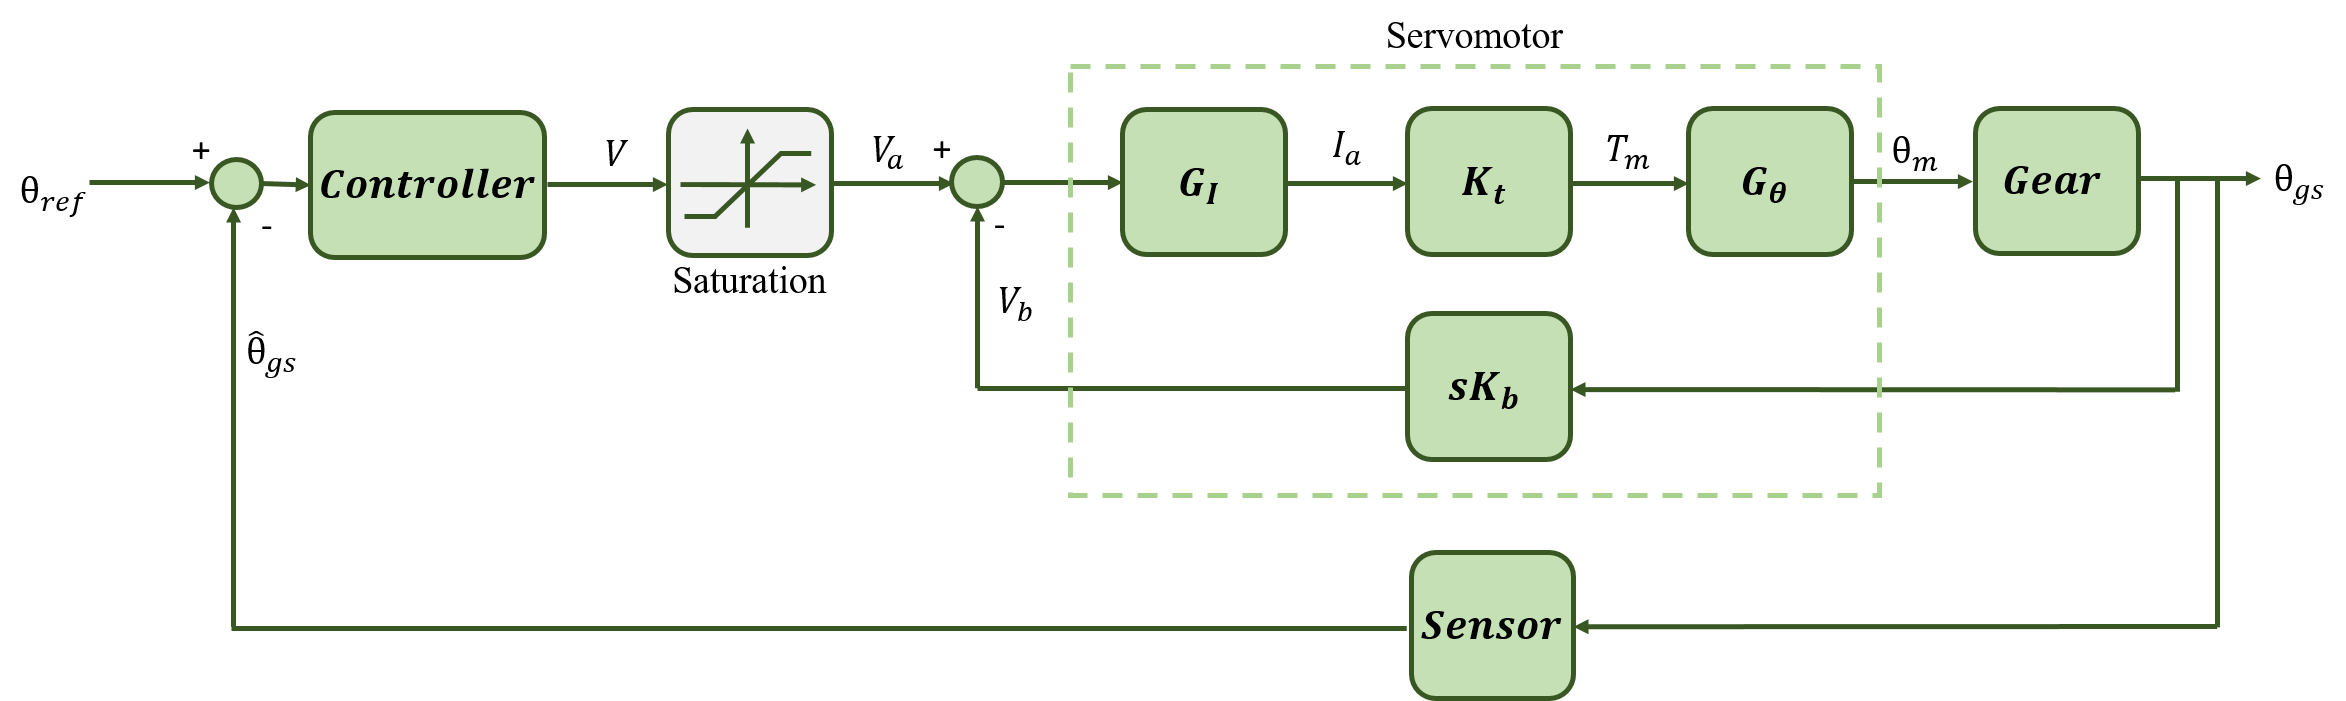
\includegraphics[scale=0.24]{../report/figures/servo+gear+noise+saturation.png}
      \end{figure}

  \end{block}
\end{frame}


%%%
%%Controller
\begin{frame}{Controller}{What controllers}
  \begin{block}{Type of control:}

	  \begin{itemize}
	  	\item PID control
	 	\begin{itemize}
	  	\item Proportional
	  	\item Derivative
	  	\item Integral
	  	\item Combination of them
	  \end{itemize}
	  \end{itemize}


  \end{block}
\end{frame}

%%%  HOW DID WE DESIGN THE CONTROLLERS?
%%Controller
\begin{frame}{Controller}{Tuning Method}
  \begin{block}{Good Gain Method:}
	  \begin{enumerate}
	  	\item Ti = $\infty$, Td = 0, Kp = 1
	  	\item Increase Kp until finding a slight overshoot
		\item Ti = 1.5$\cdot T_{out}$
		\item Td = $\frac{Ti}{4}$
	  \end{enumerate}
	  
  \end{block}
\end{frame}

%%Tuning Method
\begin{frame}{Controller}{Tuning Methods}
  \begin{block}{Good Gain Method}
  
	  \begin{enumerate}
	  	\item Ti = $\infty$, Td = 0, Kp = 1
	  \end{enumerate}
	  \begin{figure}
       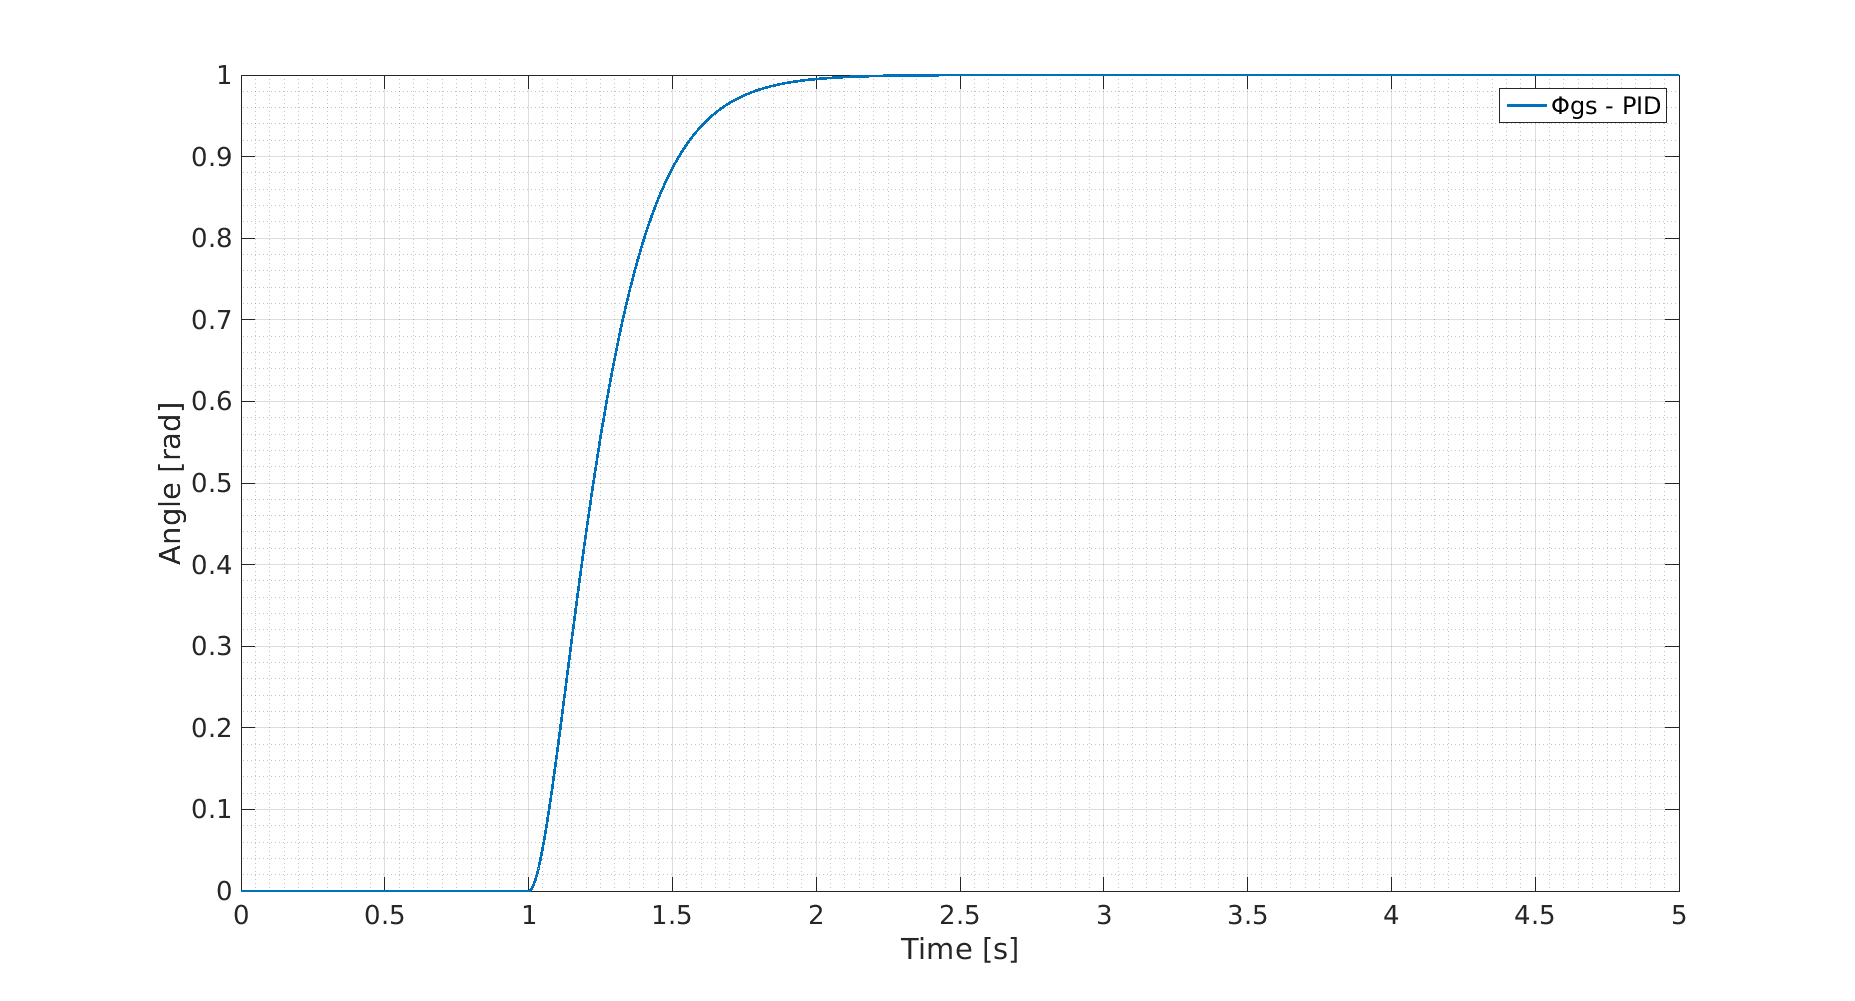
\includegraphics[scale=0.20]{../report/figures/GG1.png}
      \end{figure}
  
  \end{block}
\end{frame}

%Tuning Method
\begin{frame}{Controller}{Tuning Methods}
  \begin{block}{Good Gain Method}
  
	  \begin{enumerate}
	  \setcounter{enumi}{1}
	  	\item Increase Kp until finding a slight overshoot and well damped
	  	\begin{itemize}
	  	\item Save $T_{out}$ = Time between overshoot and undershoot
	  	\end{itemize}
	  \end{enumerate}
	  \begin{figure}
       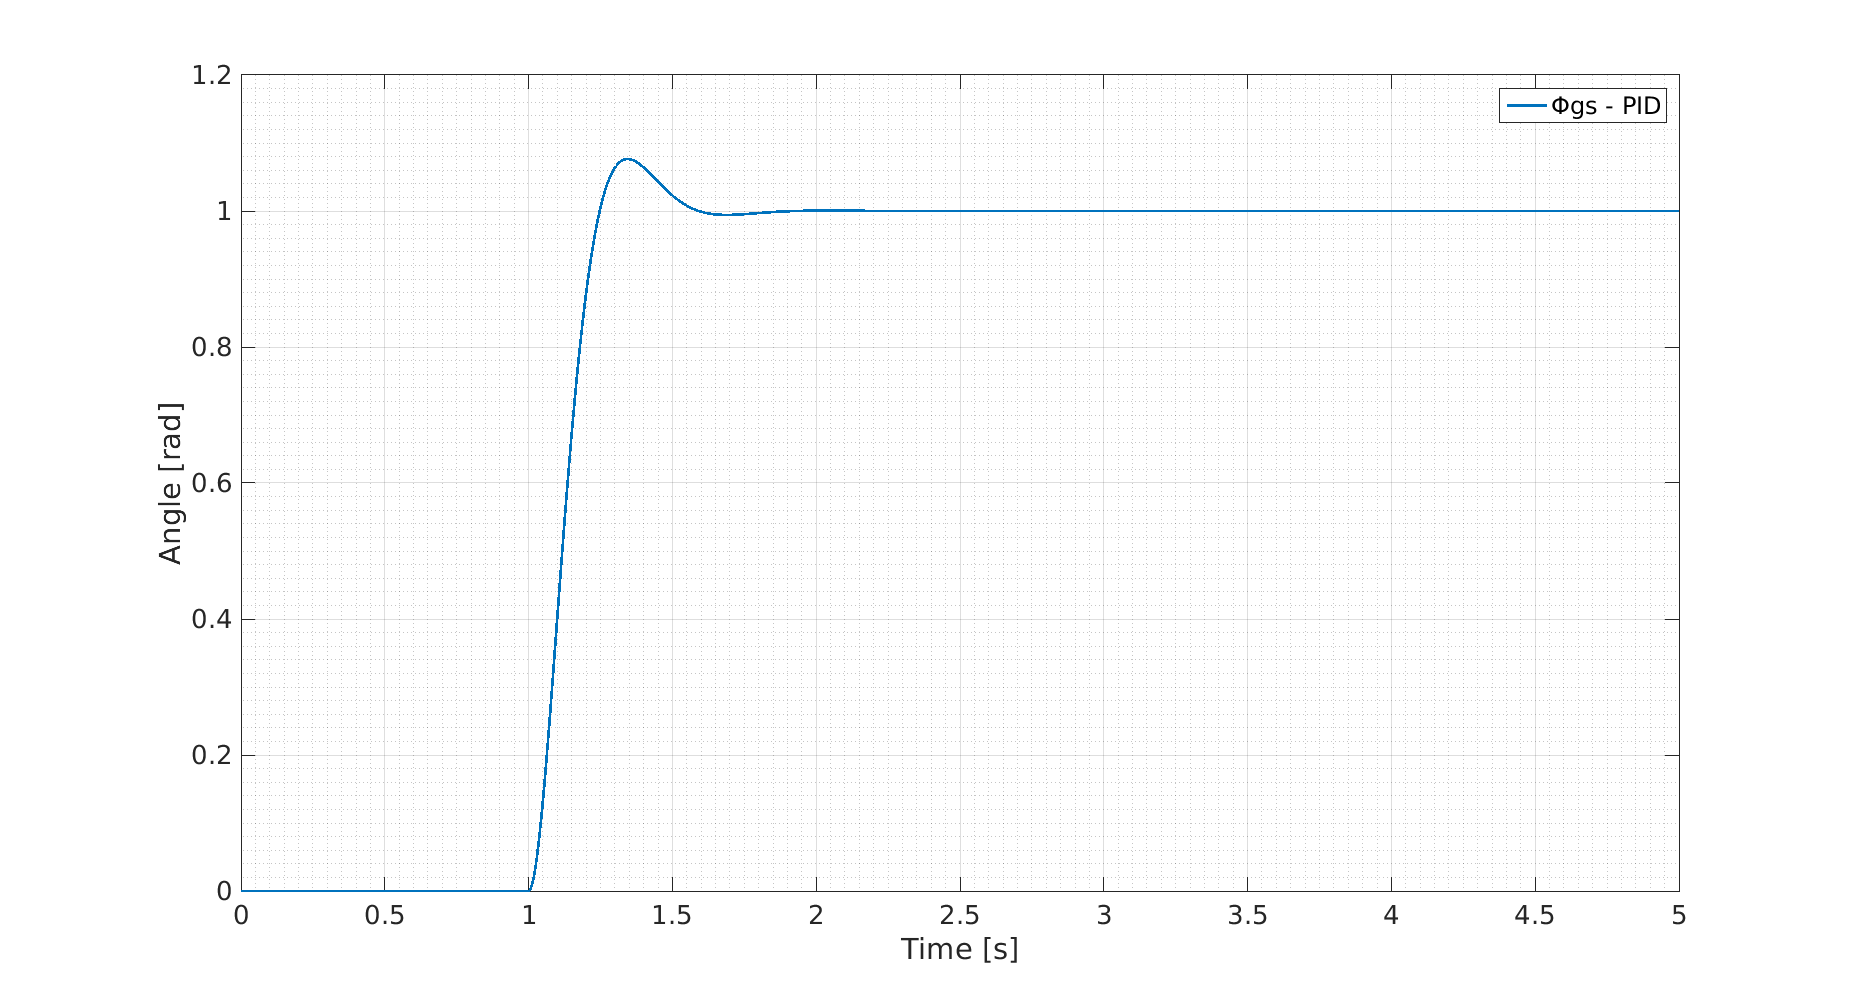
\includegraphics[scale=0.18]{../report/figures/GG2.png}
      \end{figure}
  
  \end{block}
\end{frame}

%Tuning Method
\begin{frame}{Controller}{Tuning Methods}
  \begin{block}{Good Gain Method}
  
	  \begin{enumerate}
	  \setcounter{enumi}{2}
	  	\item Ti = 1.5$\cdot T_{out}$
	  \end{enumerate}
	  \begin{figure}
       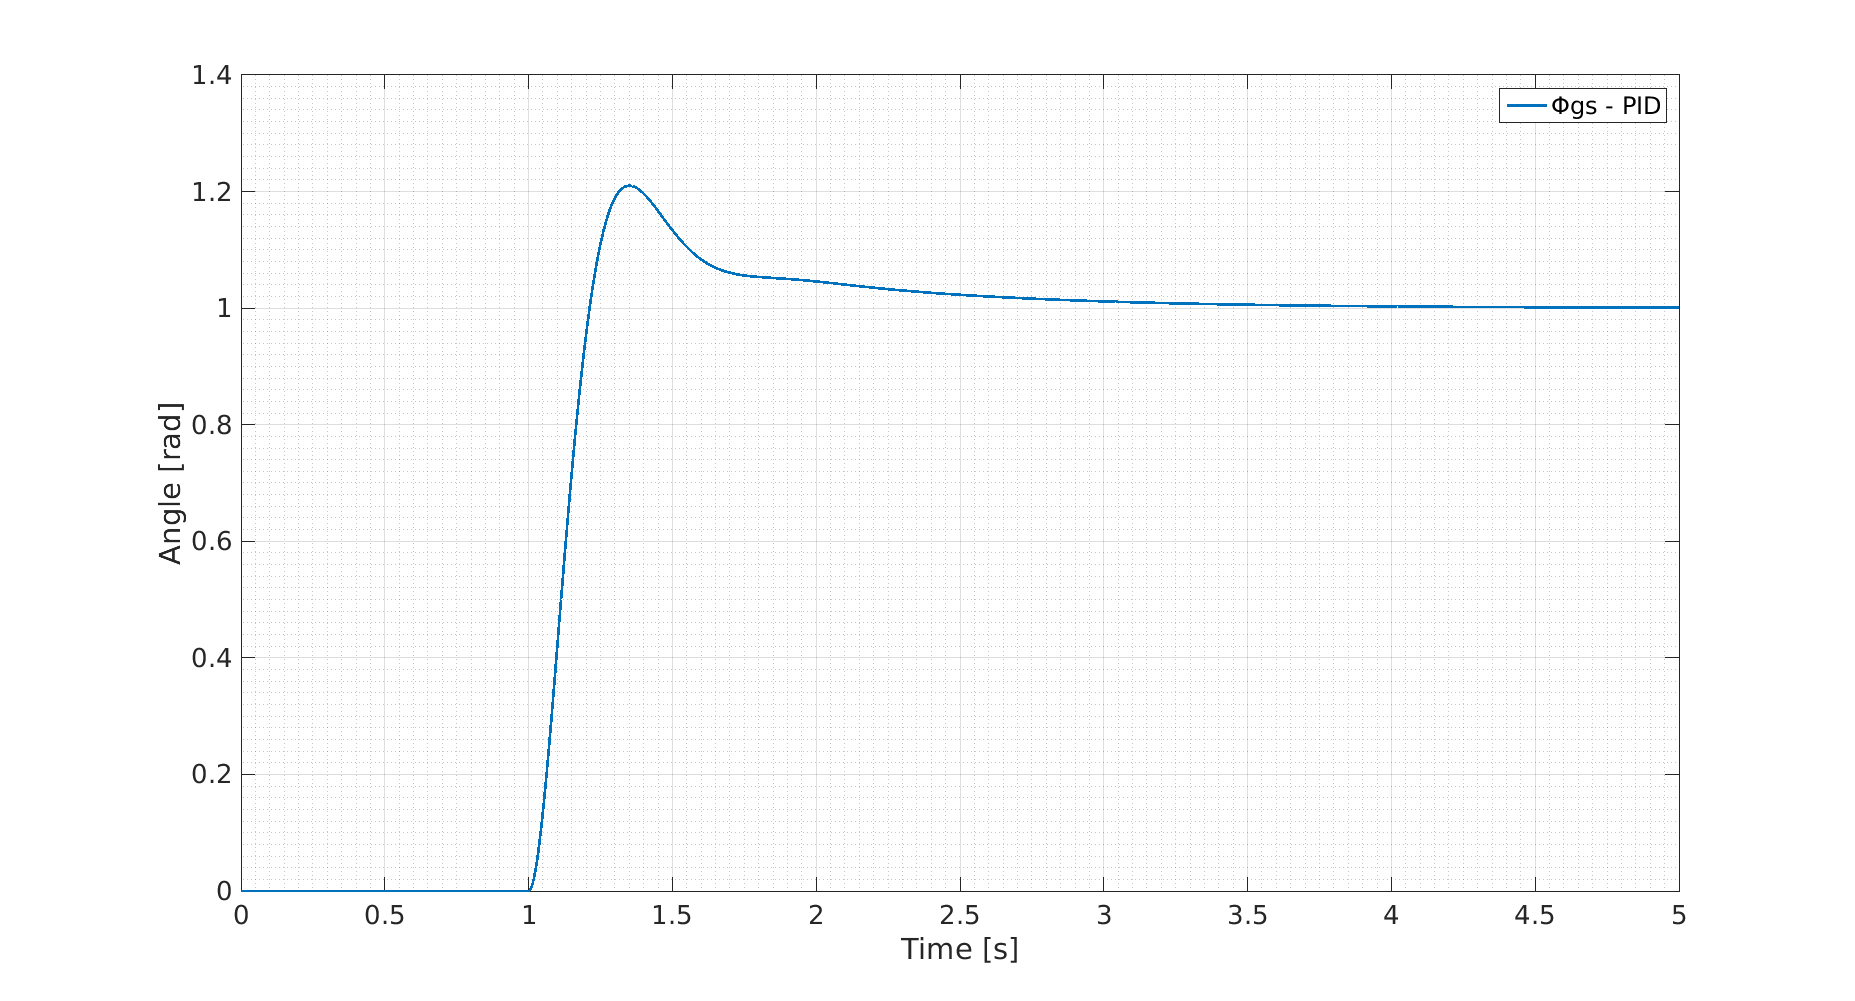
\includegraphics[scale=0.20]{../report/figures/GG3.png}
      \end{figure}
  
  \end{block}
\end{frame}



%Tuning Method
\begin{frame}{Controller}{Tuning Methods}
  \begin{block}{Good Gain Method}
  
	  \begin{enumerate}
	  \setcounter{enumi}{3}
	  	\item Td = $\frac{Ti}{4}$
	  \end{enumerate}
	  \begin{figure}
       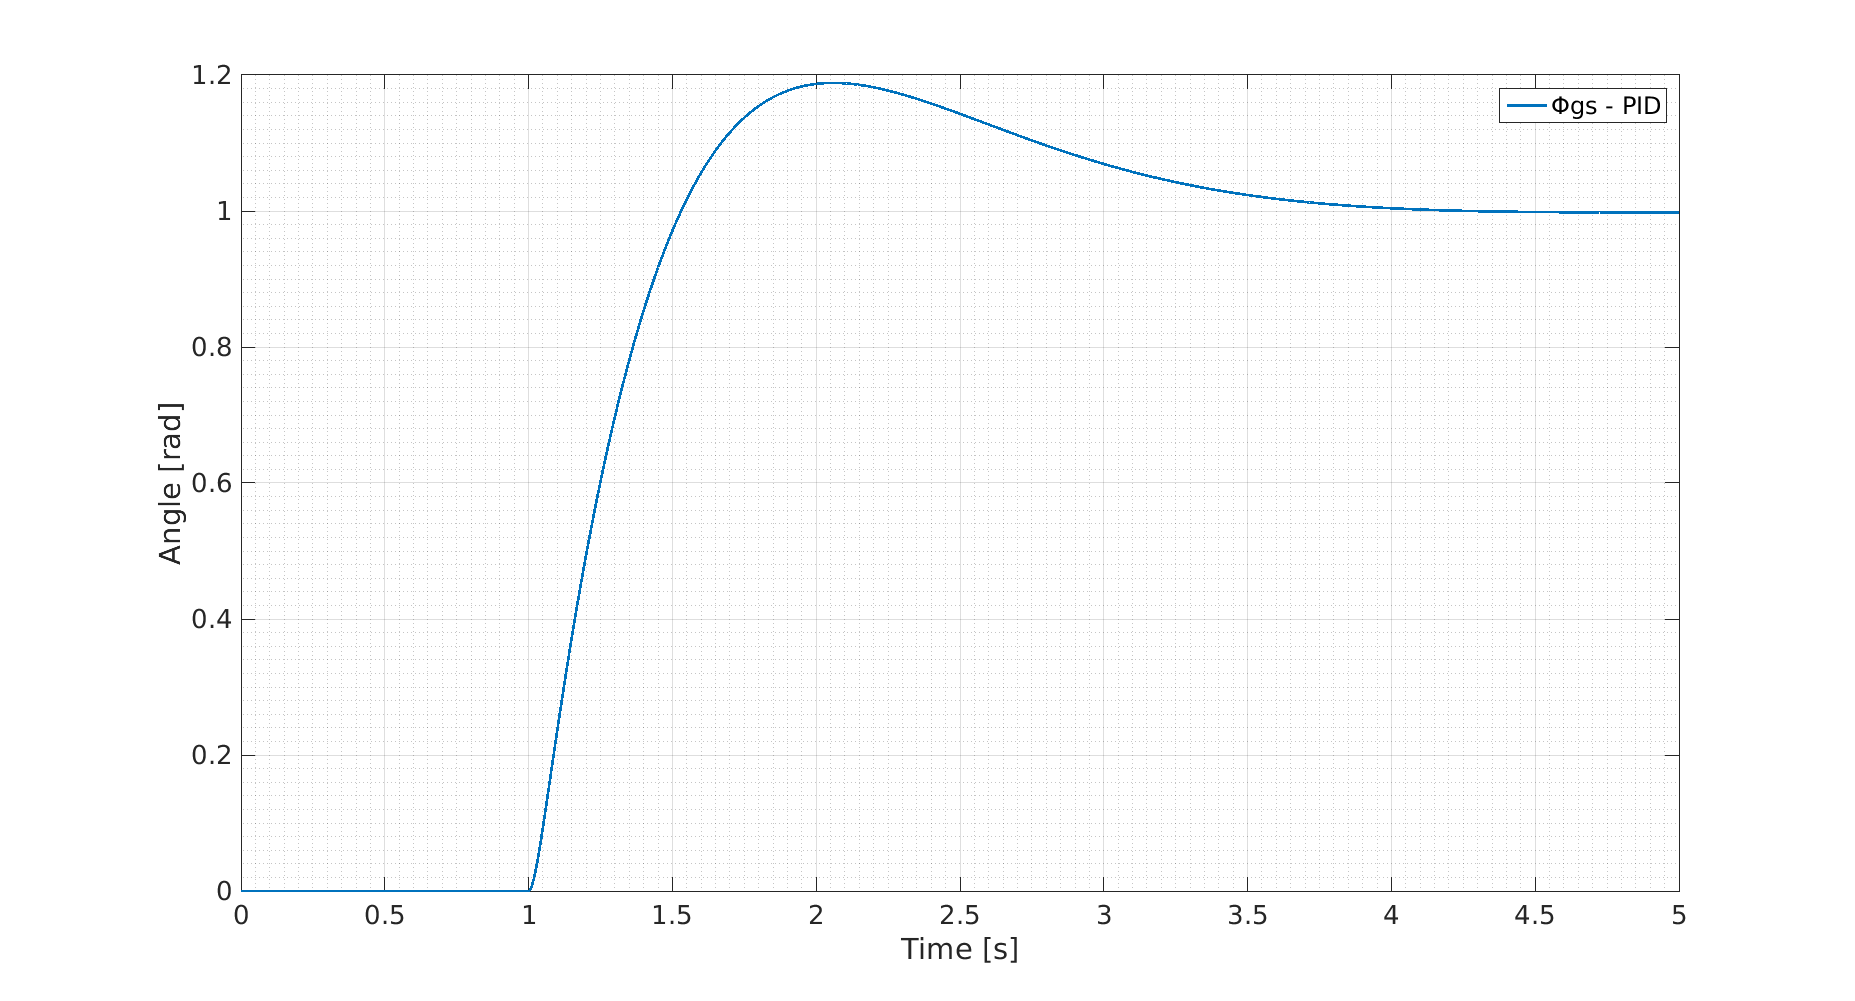
\includegraphics[scale=0.20]{../report/figures/GG4.png}
      \end{figure}
  
  \end{block}
\end{frame}


%Tuning Method
\begin{frame}{Controller}{Tuning Methods}
  \begin{block}{Good Gain Method}
  
	 \begin{itemize}
	  	\item Disadvantages:
	  \begin{itemize}
	  	\item Time consuming
	  	\item Uncertainties of the different steps	  	
	  \end{itemize}
	\end{itemize}
  
  \end{block}
\end{frame}


%%Controller
\begin{frame}{Controller}{Tuning method}
  \begin{block}{PID Simulink Box}

	  \begin{itemize}
	  \item Advantages:
	  \begin{itemize}
	  	\item Automatic Tuning Tool
	  	\item Design multiple controllers
	  	\item Adjust different parameters  	
	  \end{itemize}
	  \end{itemize}

  \end{block}
\end{frame}

%Comparison
\begin{frame}{Controller}{Comparison of step responses}
  \begin{block}{Different controllers:}
  
	  \begin{itemize}
	  	\item PI and PID - highest overshoot
	  		  \begin{itemize}
	  			\item 0.16rad and 0.19rad
	  			\item 9.17deg and 10.8deg
	  			\end{itemize}
	  	\item P and PD - no overshoot, shorter settling time, but still steady state error
	  \end{itemize}

	  \begin{figure}
        \includegraphics[scale=0.16]{../report/figures/full_comp.png}
      \end{figure}
  
  \end{block}
\end{frame}

%Comparison
\begin{frame}{Controller}{Comparison of step responses}
  \begin{block}{Different controllers with noise:}

	  \begin{itemize}
	  	\item PD faster than P
	  	\item PD reacts more to noise then P
	  \end{itemize}

	  \begin{figure}
        \includegraphics[scale=0.18]{../report/figures/PD_noise.png}
      \end{figure}
  
  \end{block}
\end{frame}

%%% CONTROLLER
%
%
%%Tuning Method
%\begin{frame}{Controller}{Tuning Methods}
%  \begin{block}{PID Simulink Box}
%
%
%	  \begin{itemize}
%	  	\item Weakness of Good Gain Method:
%	  		  \begin{itemize}
%	  	\item Time consuming
%	  	\item Uncertainties of the different steps
%	  \end{itemize}
%	  \item Advantages of PID Simulink Box
%	  \begin{itemize}
%	  	\item Automatic tuning tool
%	  	\item Include N term which avoids a "pure derivative" that reacts easily to noises
%	  \end{itemize}
%	  \end{itemize}
%  
%  \end{block}
%\end{frame}



%%Controller
%\begin{frame}{Controller}{Different controllers}
%  \begin{block}{Different controllers:}
%
%	  \begin{itemize}
%	  	\item PID control
%	 	\begin{itemize}
%	  	\item Proportional
%	  	\item Derivative
%	  	\item Integral
%	  	\item Combination of them
%	  \end{itemize}
%	  \end{itemize}
%
%
% 	  \begin{figure}
%        \includegraphics[scale=0.40]{../report/figures/control-theory-chart.jpg}
%      \end{figure} 
%  \end{block}
%\end{frame}
%%
%%Controller P
%\begin{frame}{Controller}{Different controllers}
%  \begin{block}{Proportional Term}
%
%	  \begin{itemize}
%	  	\item Output proportional to the error
%	  \end{itemize}
%
%	  \begin{figure}
%        \includegraphics[scale=0.26]{../report/figures/propor_controller.png}
%      \end{figure}
%  
%  \end{block}
%\end{frame}

%%Controller I
%\begin{frame}{Controller}{Different controllers}
%  \begin{block}{Integral Term}
%
%	  \begin{itemize}
%	  	\item Sums the error term over time
%	  	\item No steady state error
%	  	\item Cause the present value to overshoot the reference value
%	  \end{itemize}
%
%	  \begin{figure}
%        \includegraphics[scale=0.26]{../report/figures/integ_controller.png}
%      \end{figure}
%  
%  \end{block}
%\end{frame}

%%Controller D
%\begin{frame}{Controller}{Different controllers}
%  \begin{block}{Derivative Term}
%
%	  \begin{itemize}
%	  	\item Acts as a brake on the control effort
%	  	\item Highly sensitive to noise
%	  \end{itemize}
%
%	  \begin{figure}
%        \includegraphics[scale=0.26]{../report/figures/deriv_controller.png}
%      \end{figure}
%  
%  \end{block}
%\end{frame}

%%Controller PI
%\begin{frame}{Controller}{Different controllers}
%  \begin{block}{PI Controller}
%
%	  \begin{itemize}
%	  	\item Eliminate the steady state error
%	  	\item Negative impact on the speed of the response
%	  	\item Should be applied when speed is not an important parameter
%	  \end{itemize}
%
%	  \begin{figure}
%        \includegraphics[scale=0.26]{../report/figures/PI_controller.png}
%      \end{figure}
%  
%  \end{block}
%\end{frame}
%
%
%%Controller PD
%\begin{frame}{Controller}{Different controllers}
%  \begin{block}{PD Controller}
%
%	  \begin{itemize}
%	  	\item Why is PD alone good?
%	  \end{itemize}
%
%	  \begin{figure}
%        \includegraphics[scale=0.26]{../report/figures/PD_controller.png}
%      \end{figure}
%  
%  \end{block}
%\end{frame}
%
%%Controller PID
%\begin{frame}{Controller}{Different controllers}
%  \begin{block}{PID Controller}
%
%	  \begin{itemize}
%	  	\item Eliminate steady state error
%	  	\item Fast response
%	  	\item Higher stability
%	  	\item (Derivative Term) Reduction of the overshoot and oscillations
%	  \end{itemize}
%
%	  \begin{figure}
%        \includegraphics[scale=0.26]{../report/figures/PID_controller.png}
%      \end{figure}
%  
%  \end{block}
%\end{frame}






\subsection{Simulation}

\begin{frame}{Simulation}{LOS Coverage Map}
  \begin{block}{Parameters taken into account for map simulation:}

	  \begin{itemize}
	  	\item Terrain elevation
	  	\item Curvature of the Earth
	  	\item Altitude of UA and GS
	  \end{itemize}

	  \begin{figure}
        \includegraphics[scale=0.26]{../report/figures/dk_map.png}
      \end{figure}
  
  \end{block}
\end{frame}

\begin{frame}{Simulation}{LOS Coverage Map}
  \begin{block}{Working Principle}
	  \begin{itemize}
	  	\item Import topography map
	  	\item Input GS and UA altitude
	  	\item Choose GS and UA locations on map to plot LOS distance
	  	\item Choose GS location on map to plot LOS coverage map
	  \end{itemize}
  \end{block}
\end{frame}

\begin{frame}{Simulation}{LOS between UA and GS} 
  	\begin{figure}
        \includegraphics[scale=0.29]{../report/figures/los_2points.png}
    \end{figure}
\end{frame}

\begin{frame}{Simulation}{LOS Coverage Map} 
  	\begin{figure}
        \includegraphics[scale=0.40]{../report/figures/los_odense.png}
    \end{figure}
\end{frame}

\begin{frame}{Simulation}{2D UAS}
	\begin{block}{2D UAS Block Diagram}
		\begin{itemize}
		  	\item Cartesian system (Simplistic)
		  	\item 1 DoF - azimuth angle ($\theta$)
		  	\item Compute optimal azimuth angle for UA and GS 
		\end{itemize}

		\begin{figure}
	        \includegraphics[scale=0.32]{figures/2D_system.png}
	    \end{figure}
    \end{block}
\end{frame}

\begin{frame}{Simulation}{3D UAS}
  \begin{block}{3D UAS Block Diagram}
	\begin{itemize}
	  	\item Realistic Earth Model - WGS84
	  	\item Curvature of the Earth
	  	\item Relief of Earth's surface 
	  	\item Real GPS position: latitude, longitude and altitude
	\end{itemize}

	\begin{figure}
		\includegraphics[scale=0.33]{figures/3D_system.png}
	\end{figure}
  \end{block}
\end{frame}

\section{LOS Coverage Map}\label{sec:los_map}
A point of interest of the project is to know if there is Line-Of-Sight (LOS) between the ground station (GS) and the drone. This has been done on a topographic map which takes into account:

\begin{itemize}
	\item Terrain elevation
	\item Curvature of the Earth
	\item Height of receiver and transmitter
\end{itemize}

\subsection{Mathematical Background}
Should this be here ??? or relate with something from the Frames Chapter ???

\subsection{Initial Step}
In this sense, a MATLAB script has been addressed which at first imports a Web Map Service (WMS) to load the topographic map. The map captures the terrain in Denmark and some of its surroundings as seen in Figure \ref{fig:dk_map}.

\begin{figure}[h]
	\centering
	\includegraphics[scale=2]{figures/denmark.jpg}
	\caption{Topographic map of Denmark}
   	\label{fig:dk_map}
\end{figure}

\subsection{LOS Distance}
Given the map and the topographic data in Figure \ref{fig:dk_map}, now it is possible to input the desired points for the GS and the drone. As mentioned above, there are some parameters taken into account for plotting the LOS distance between the two points of interest. This distance can be seen in Figure \ref{fig:los_2p}, where the LOS is lost after 45 kilometers from the GS.

\begin{figure}[h]
	\centering
	\includegraphics[scale=0.75]{figures/los_2p.jpg}
	\caption{LOS between GS and drone \\ X axis - LOS distance [m] \\ Y axis - Altitude [m]}
   	\label{fig:los_2p}
\end{figure}

\subsection{Coverage Map}
Moving further, for the same map (Figure \ref{fig:dk_map}) a location for the GS can be chosen, such that it will result into a LOS area (white zone) as seen in Figure \ref{fig:los_area}. This area is also referred as the LOS coverage map.

\begin{figure}[h]
	\centering
	\includegraphics[scale=2.5]{figures/coverage_map.jpg}
	\caption{LOS Coverage Map from the GS}
   	\label{fig:los_area}
\end{figure}

It can be observed from Figure \ref{fig:los_area} that in some areas of the map there is no visibility, due to higher terrain elevation. This can be overcome by increasing the GS and/or drone altitude, such that we achieve LOS.  


!!! !!! !!! NEED EXAMPLE OF COAST !!! !!! !!!

\subsection{Working Principle}
Taking into account that a MATLAB script has been achieved, a thourough working principle has to be addressed in the following steps:
\begin{itemize}
	\item Aquire topography map 
	\item Input GS and drone altitudes
	\item Choose locations for GS and drone on (click) the map in order to plot LOS distance
	\item Choose (click) location of the GS in order to plot LOS coverage map
\end{itemize}
\newpage
\section{2D System Simulation}
As it is mentioned earlier, the whole idea of the project is to make the antenna of the drone and the ground stations point at each others. To achieve this its needed to know the angle of the antennas and their optimal angle, which is when they point exactly at each others. To be able to point the antennas towards each others two controllers will be implemented. In this section an algorithm to calculate the optimal angle will be introduced. Furthermore the implementation of the controllers will be explained.
\subsection{Scenario}
In Figure \ref{fig:drone_gs} it is shown a scenario where the antennas of both GS and drone change after some periods of time. In the top part of the figure it shows the angle of the drone ($\theta_{d}$) and the optimal angle ($\theta_{opt\_d}$) that the antenna want to be in. In the lower part of the figure it shows the angle of the ground station ($\theta_{gs}$) and the optimal angle ($\theta_{opt\_gs}$). 

\begin{figure}[h]
	\centering
	
	\includegraphics[scale=0.45]{figures/drone_gs_ex_1.jpg}
	\caption{Example of a drone-gs scenario}
	\label{fig:drone_gs}
\end{figure}

As it is seen on the figure at time k the antenna of the drone ($\theta_d (k)$) is not equal the optimal angle ($\theta_{opt\_d}(k)$). The same goes with the $\theta_{gs}(k)$ and the optimal angle $\theta_{opt\_gs}(k)$. As the drone moves further on the X-axis the angle of the ground station and the drone goes closer to the optimal angle. 

\subsection{System overview}
The system presented is a Multiple Input Multiple Output (MIMO) system, such that in this case there are 4 inputs and 2 outputs. The system is shown in figure \ref{fig:2d_system}. 

\begin{figure}[h]
	\centering
	\includegraphics[scale=0.42]{figures/2d_system.png}
	\caption{2D sytem overview}
	\label{fig:2d_system}
\end{figure}
The first block of the system takes as inputs the parameters below and computes the optimal angles for the ground station ($\theta\_opt\_gs$) and drone ($\theta\_opt\_d$) antennas, such that a strong communication link is achieved. \\

\noindent The 2 outputs, of the first block, that it is needed to control are:
\begin{itemize}
	\item Drone's antenna angle ($\theta_{d}$)
	\item Groundstation's antenna angle ($\theta_{gs}$)
\end{itemize}

\noindent The system's inputs are as follows:
\begin{itemize}
	\item Drone's antenna angle ($\theta_{d}$)
	\item Groundstation's antenna angle ($\theta_{gs}$)
	\item Drone position ($x_{drone},y_{drone}$)
	\item Groundstation position ($x_{gs},y_{gs}$)
\end{itemize}

\subsection{Optimal angle}
The right part of figure \ref{fig:2d_system} shows two PD controllers where each of them have a servomotor connected. The PD controller is explained in chapter \ref{dcmotor_circuit} and the servo is explained in chapter \ref{ch:simulation}. The left block have two output which is $\theta\_opt\_d$ and $\theta\_opt\_gs$. They are the optimal angle that the drone and ground station need to have to be pointing at each other (Figure \ref{fig:drone_gs}). The PD controllers purpose is to make the servomotors rotate the antenna to the correct position. The PD controllers take the error ($\theta\_opt\_d$ -$\theta\_d$) for the drone and ($\theta\_opt\_gs$ - $\theta\_gs$ for the ground station, and make the servomotors rotate the antenna to the correct position. When the error is zero, which means the input to the PD controller is zero, the antennas are at the correct angles.   

\subsection{Simulations}
To verify that the 2D simulations work, some simulations are made. In the first simulation the drone is simulated by starting in (0,50) and going to (100,50), which means that the drone is only moving in the x-axis. The simulation is shown in figure \ref{fig:gs_angle_vs_optimal} where the top one is showing the Drone angle versus the optimal angle and the bottom one is showing the ground station angle versus the optimal one. 

\begin{figure}[h]
	\centering
	\includegraphics[scale=0.6]{figures/gs_angle_vs_optimal.png}
	\caption{Ground station angle vs optimal}
	\label{fig:gs_angle_vs_optimal}
\end{figure}

In this plot the angle is shown in degree to make it easier to understand. The blue line in both plots is respectively the drone and the ground stations antenna angle. They both start in 0 degree and have no initial starting point. Here it takes about 46 seconds for the drones antenna to be at the optimal angle and in the other case it takes about 17 seconds for the ground station antenna to turn to the optimal angle. But when they reached their optimal angle, the controller holds the antennas to the optimal angle. 
\newpage


\section{3D System Unmanned Aircraft System}\label{sec:3d_sim}

\paragraph{}The 2D simulation in the former section serves its purpose as a simple case scenario that gives an insight of how to approach the problem, but it differs greatly from reality. Besides from the obvious lack of the 3rd dimension, another flaws need to be addressed, such as using real earth model (WGS84) instead of a simple cartesian coordinate plane  and taking into account the curvature and relief of the Earth's surface. However, the same geometrical principles are used, as long as the proper frame transformations are derived (Chapter \ref{ch:frames}).

\paragraph{} Figure \ref{fig:diagram3D} shows the actual augmented block diagram used in MATLAB Simulink in order to run this simulation. It is mainly based in the following steps:
\begin{enumerate}
\item{Read Ground Station and Drone GPS position.}
\item{Calculate optimal angles (reference), error signal and other parameters. This requires from frames transformation and other functions, and it is performed inside the MATLAB function block, which will be explained later on.}
\item{Input the error signal into the controller.}
\item{Limit the output signal from the controller by the use of the saturation box.}
\item{Input the output signal into Servo-motor model box. This model can be seen in Figure \ref{fig:servomotor3D}, whose parameters have been explain in Chapter \ref{sec:servo_model}.}
\item{Feedback the output angle into the MATLAB function block and repeat again from step 2.}
\end{enumerate}

\subsection*{MATLAB Function}
\paragraph{}Firstly note that, as explain in section \ref{sec:opt_angle}, this function is duplicated since almost the same calculations for Ground Station and Drone have to be done, being the only diference the reference (origin) for the local NED transformation.
The Ground station version will transform the Drone GPS coordinates to ECEF and then to the local NED Frame with respect to the Ground Station position. The Drone version do the analgous calculation but the NED Frame will be with respect to the Drone position.

\paragraph{}After this, the \textbf{optimal} or {reference} angles will be calculated according to the equations \ref{eq:OptGS} and the error signal obtained by substracting this calculated angle with the current angle position of the antenna, which comes from the outer loop feedback.

\paragraph{} Some scopes and blocks come out of the output signals of these funcions with mainly debugging and plotting purposes, having no impact in the actual performance of the system. 

\begin{figure}[h]
	\centering
	\includegraphics[width=1\textwidth]{figures/servomotor_3D.png}
	\caption{Servo-motor Block Diagram}
   	\label{fig:servomotor3D}
\end{figure}

\clearpage

\begin{sidewaysfigure}[h]
	\centering
	\includegraphics[width=1.1\textwidth,height=1.1\textheight,keepaspectratio]{figures/diagram_3D.png}
	\caption{Block Diagram for 3D Simulation}
   	\label{fig:diagram3D}
\end{sidewaysfigure}

\clearpage


\subsection*{Simulations}

In the following chapter, the results of 4 different simulations will be presented, each of them exampling some specific characteristics. These will consist in short straight paths between two points and they will use the 3D Unmmaned Aircraft System showed in Figure \ref{fig:diagram3D}.

However, in order to perform this simulations some parameters need to be set and some considerations noted:

\begin{itemize}
\item{The antenna used for the simulation is the same for both GS and UA, and it has the specifications defined in table \ref{table:2}.}
\begin{table}[h]
	\centering
	\begin{tabular}{|c||c|}
		\hline
		Parameter & GS\\ \hline\hline
		Type & Parabolic\\ \hline
		Polarization & Linear\\ \hline
		Frequency [GHz] & $2.4$\\ \hline
		Gain [dB] & $27.6$\\ \hline
		HPBW/$H(^{\circ})$ & $14$\\ \hline
		HPBW/$V(^{\circ})$ & $14$\\ \hline
	\end{tabular}
	\caption{Antenna Specifications}
	\label{table:2}
\end{table}
\item{It is assumed that the Moving Angle System of both the UA and GS use the same servo-motor, defined in Chapter \ref{sec:servo_model}.}
\item{The controller used will be defined in each of the simulations.}
\item{The saturation voltage threshold going into the servomotor is set to +5v and -5v.}
\item{The measurement noise at the output will be modelled as a Gaussian White Noise with a noise power of 0.0001}
\item{No power threshold fixed in the receiver.}
\item{The UA will be facing always the end point of the path during the flight}
\end{itemize}




\chapter{Results and Discussion}\label{ch:results}
Taking into account the 3D simulation discussed in Chapter \ref{ch:sim} 
\section{Scenario 1}\label{sec:scenario1}
% The purpose of this scenario is to simulate 4 controllers in order to compare them using the map in Figure \ref{fig:s1_map}. 

% \begin{figure}[H]
% 	\hfill
% 	\subfigure[UAS Map Positioning]{\includegraphics[scale=0.33]{figures/s1_p_map.png}}
% 	\hfill
% 	\subfigure[LOS and Distance]{\includegraphics[scale=0.33]{figures/s1_los.png}}
% 	\hfill
% 	\caption{Mountain Scenario}
% 	\label{fig:s1_map}
% \end{figure}

% \subsection{UA}
% In Figure \ref{fig:s1_ua} the angle tracking of the UA antenna can be seen.

% \begin{figure}[H]
% 	\hfill
% 	\subfigure[UAS Map Positioning]{\includegraphics[scale=0.33]{figures/scenario_1_map.png}}
% 	\hfill
% 	\subfigure[LOS and Distance]{\includegraphics[scale=0.33]{figures/scenario_1_los.png}}
% 	\hfill
% 	\caption{Mountain Scenario}
% 	\label{fig:s1_map}
% \end{figure}

% \subsection{GS}
% In Figure \ref{fig:s2_gs} the angle tracking of the GS antenna can be seen.

% \begin{figure}[H]
% \hfill
% \subfigure[UAS Map Positioning]{\includegraphics[scale=0.33]{figures/scenario_1_map.png}}
% \hfill
% \subfigure[LOS and Distance]{\includegraphics[scale=0.33]{figures/scenario_1_los.png}}
% \hfill
% \caption{Mountain Scenario}
% \label{fig:s1_map}
% \end{figure}

% \subsection{Power}
% In Figure \ref{fig:s2_power} the power at the receiver antenna of the GS antenna can be seen.

% \begin{figure}[H]
% \hfill
% \subfigure[UAS Map Positioning]{\includegraphics[scale=0.33]{figures/scenario_1_map.png}}
% \hfill
% \subfigure[LOS and Distance]{\includegraphics[scale=0.33]{figures/scenario_1_los.png}}
% \hfill
% \caption{Mountain Scenario}
% \label{fig:s1_map}
% \end{figure}

\newpage
\section{Scenario 2 - Curvature of the Earth}\label{sec:scenario2}
The purpose of this scenario is to show how the curvature of the Earth comes into play, as seen on the map in Figure \ref{fig:s2_map}. In this case, the UA starts near the GS and moves away from it in a somewhat straight line. To be mentioned that a PD controller is used in simulation of the UAS in this scenario.

\begin{figure}[H]
	\centering
	\subfigure[UAS Map Positioning]{\includegraphics[scale=0.37]{figures/s2_map.png}}
	\subfigure[UAS Map Zoom]{\includegraphics[scale=0.31]{figures/s2_zoom.png}}
	\\
	\subfigure[LOS and Distance]{\includegraphics[scale=0.53]{figures/s2_los.png}}
	\hfill
	\caption{Curvature Scenario}
	\label{fig:s2_map}
\end{figure}


\subsection*{UA and GS Tracking Angles}
In this scenario, the UA is on the left side of the GS as is illustrated on Figure \ref{fig:s2_map}. As was explained in Scenario 1 (Section \ref{sec:scenario1}), due to the chosen body frame coordinate of the GS, the optimal azimuth angle is always negative. On the other hand, the UA is flying away from the GS in a straight line which results in an almost constant azimuth angle as it can be seen in Figure \ref{fig:s2_gs}. 

The optimal elevation angle has a slightly decrease (bigger than in the previous scenario) during the whole movement. It starts with a higher value because the UA is close to the GS. While the UA is progressing towards the end point, the distance between both devices grows which causes a decrease in the antenna's $\phi_{OPTIMAL}$ angle. However, in this situation, the $\phi_{OPTIMAL}$ becomes negative on the 70th sample, which means that, in the point of view of the GS, it has a bigger altitude compared to the UA one. The $\phi_{OPTIMAL}$ can achieve negative values because the curvature of the Earth was taken into account.

\begin{figure}[H]
	\centering
	\includegraphics[scale=0.75]{figures/s2_gs.png}
	\caption{Azimuth and elevation angles of GS following the optimal angle}
	\label{fig:s2_gs}
\end{figure}


\paragraph{}
The optimal and UA azimuth angles in Figure \ref{fig:s2_ua} have the same behaviour, despite of the opposed values that they show. This is due to the fact that different conventions applied in each variable (Section \ref{sec:scenario1}), the lines are not overlapped but they represent the same angle.

Previously explained, the UA is flying away from the GS which also implies that the reference of the body frame is pointing to the end point. Therefore, it demands that the antenna of the UA is pointing back in order to keep the connection with the GS. 

The elevation angle has a similar behaviour to the one of the GS. However, in this case, the antenna of the UA is pointing down because the altitude of the UA is higher than the GS. During the flight the angle of the antenna is increasing, moving towards zero meaning that the UA is going over the horizon.


\begin{figure}[H]
	\centering
	\includegraphics[scale=0.75]{figures/s2_ua.png}
	\caption{Azimuth and elevation angles of UA following the optimal angle}
	\label{fig:s2_ua}
\end{figure}


\subsection*{Signal Power}
In Figure \ref{fig:s2_power} the power at the receiver antenna of the GS antenna can be seen. In the beginning the signal power at the receiver is weak (-100dBm) because the antennas are not pointing at each other. Although, after 4 samples, the connection is accomplished and the power reaches its maximum (-35dBm). During the flight the signal power gradually decreases, because the aircraft is moving away from the ground station. 

\begin{figure}[H]
	\centering
	\includegraphics[scale=0.75]{figures/s2_power.png}
	\caption{Power at the receiver's antenna at both ends}
	\label{fig:s2_power}
\end{figure}


\newpage
\section{Scenario 3 - Above the GS}\label{sec:scenario3}
The scenario 3 run in a short distance from north to south, where the Unmanned Aircraft flies over the Ground Station. The UA starts and ends 6km from the GS from North to South as can be seen in the Figure \ref{fig:s3_map}(a). The distance between the 2 devices at every sample is shown in the Figure \ref{fig:s3_map}(b). As followings in former graphs, the blue circles mean that there is line of sight between them. 


\begin{figure}[H]
	\centering
	\subfigure[UAS Map Positioning]{\includegraphics[scale=0.38]{figures/s3_map.png}}
	\subfigure[UAS Map Zoom]{\includegraphics[scale=0.32]{figures/s3_zoom.png}}
	\\
	\subfigure[LOS and Distance]{\includegraphics[scale=0.53]{figures/s3_los.png}}
	\caption{Above the GS Scenario}
	\label{fig:s3_map}
\end{figure}

\subsection*{UA and GS Tracking Angles}
In the start of the simulation, both Ground Station and Unmanned Aircraft calculte their azimuth and elevation angles necessary to point at each other (optimal angles). A small delay can be seen in Figure \ref{fig:s3_gs} for the azimuth angle of the Ground Station to reach its reference angle. This delay is the result of the starting point of the antennas, being 0$^{\circ}$, and the motions of the moving angles system. Hence, no delay can be observed for the azimuth angle of the UA and the elevation angles of both devices, by cause of having 0 degree for their optimal angle and their starting angle (Figures \ref{fig:s3_ua} and \ref{fig:s3_gs}).

The crossing point can be clearly observed on their elevation angles, where the speed of the aircraft is directly related to their sudden changes, resulting in a quick peak of almost -90 and 90 degrees for respectvively, the UA and the GS. 

\begin{figure}[H]
	\centering
	\includegraphics[scale=0.8]{figures/s3_gs.png}
	\caption{Azimuth and elevation angles of GS following the optimal angle}
	\label{fig:s3_gs}
\end{figure}

\begin{figure}[H]
	\centering
	\includegraphics[scale=0.8]{figures/s3_ua.png}
	\caption{Azimuth and elevation angles of UA following the optimal angle}
	\label{fig:s3_ua}
\end{figure}

\subsection*{Signal Power}
In Figure \ref{fig:s3_power}, the power in the receiver is growing in time. While the UA is moving in the direction of the GS, the distance between them decreases and thus the power in the receiver increases. However, a drop-off can be seen at their crossing point. The reference angle is changing too fast for the Moving angle system to reach it in time. Thus, at their crossing point, the antennas of the two devices will not point directly at each other, having for effect to decrease the power in the receiver.

\begin{figure}[H]
	\centering
	\includegraphics[scale=0.8]{figures/s3_power.png}
	\caption{Power at the receiver's antenna (GS)}
	\label{fig:s3_power}
\end{figure}
\section{Scenario 4}\label{sec:scenario4}
The purpose of this scenario is to show what can happen when the UAS loses line-of-sight because of a mountain, as seen on the map in Figure \ref{fig:s4_map}. Also, the controller used in the simulation is a PD controller.

\begin{figure}[H]
\hfill
\subfigure[UAS Map Positioning]{\includegraphics[scale=0.33]{figures/scenario_4_map.png}}
\hfill
\subfigure[LOS and Distance]{\includegraphics[scale=0.33]{figures/scenario_4_los.png}}
\hfill
\caption{Mountain Scenario}
\label{fig:s4_map}
\end{figure}

\subsection{UA}
In Figure \ref{fig:s4_ua} the angle tracking of the UA antenna can be seen.

\begin{figure}[H]
\centering
\includegraphics[scale=0.75]{figures/scenario_4_ua.png}
\caption{Azimuth and elevation angles of UA following the optimal angle}
\label{fig:s4_ua}
\end{figure}

\subsection{GS}
In Figure \ref{fig:s4_gs} the angle tracking of the GS antenna can be seen.

\begin{figure}[H]
\centering
\includegraphics[scale=0.75]{figures/scenario_4_gs.png}
\caption{Azimuth and elevation angles of GS following the optimal angle}
\label{fig:s4_gs}
\end{figure}

\subsection{Power}
In Figure \ref{fig:s4_power} the power at the receiver antenna of the GS antenna can be seen.

\begin{figure}[H]
\centering
\includegraphics[scale=0.75]{figures/scenario_4_power.png}
\caption{Power at the receiver's antenna (GS)}
\label{fig:s4_power}
\end{figure}

\chapter{Conclusion}\label{ch:conclusion}
In case you have questions, comments, suggestions or have found a bug, please do not hesitate to contact me. You can find my contact details below.
  \begin{center}
    Jesper Kjær Nielsen\\
    \href{mailto: jkn@es.aau.dk}{jkn@es.aau.dk}\\
    \href{http://kom.aau.dk/~jkn}{http://kom.aau.dk/\textasciitilde jkn}\\
    Fredrik Bajers Vej 7\\
    9220 Aalborg Ø
  \end{center}


\printbibliography
\label{bib:mybiblio}
\appendix
% \section{Controller System}\label{sec:controller_sys}
\href{http://ctms.engin.umich.edu/CTMS/index.php?example=MotorPosition&section=SystemModeling}{DC Motor Position: System Modeling}

\subsection{Physical Setup}
A common actuator in control systems is the DC motor. It directly provides rotary motion and, coupled with wheels or drums and cables, can provide translational motion. The electric equivalent circuit of the armature and the free-body diagram of the rotor are shown in the following figure. 

\begin{figure}[h!]\label{fig:motor_model}
	\centering
	\includegraphics[width=0.7\textwidth]{figures/motor.png}
	\caption{DC Servo Motor}
\end{figure}

From the figure above, we can derive the following governing equations based on Newton's 2nd law and Kirchhoff's voltage law.

\begin{equation}
	J \dot{\dot{\Theta}} + b\dot{\Theta} = Ki \\
	L\frac{di}{dt} + Ri = V - K\dot{\Theta}
\end{equation}

\subsection{Transfer Function}
Applying the Laplace transform, the above modeling equations can be expressed in terms of the Laplace variable s. On the link they dont consider initial condition and we want them.

\begin{equation}
	\mathscr{L}\{J \dot{\dot{\Theta}}\}  + \mathscr{L}\{b\dot{\Theta}\} = \mathscr{L}\{Ki\}
\end{equation}

The result become:
\begin{align*}
	& L(I(s)s-i(0)) + RI(s) = V(s) - K(s\Theta (s) - \theta (0)) \\
	& \Rightarrow I(s)(Ls+R) = V(s) - K(s\Theta (s) - \theta (0)) +Li(0) \\
	& \Rightarrow I(s) = \frac{V(s) - K(s\Theta (s) - \theta (0)) +Li(0)}{(Ls+R)}
\end{align*}

Kirchoffs voltage law:
\begin{equation*}
	\mathscr{L}\{L\frac{di}{dt}\} + \mathscr{L}\{Ri\} = \mathscr{L}\{V\} - \mathscr{L}\{K\dot{\Theta}\}
\end{equation*}

The result become:
\begin{align*}
	& J(s^2 \Theta(s) - s\theta (0) - \dot{\theta} (0)) +b(s\Theta (s)-\theta (0)) = KI(s) \\
	& Js^2 J\Theta(s) - Js\theta (0) - J\dot{\theta} (0) +b(s\Theta (s)-\theta (0) = KI(s) 
\end{align*}

And with I(s) inserted:
\begin{align*}
	& Js^2 J\Theta(s) - Js\theta (0) - J\dot{\theta} (0) +b(s\Theta (s)-\theta (0) = K (\frac{V(s) - K(s\Theta (s) - \theta (0)) +Li(0)}{(Ls+R)}) \\
	& (Js^2 J\Theta(s) - Js\theta (0) - J\dot{\theta} (0) +b(s\Theta (s)-\theta (0))(Ls+R) =  K(V(s) - K(s\Theta (s) - \theta (0)) +Li(0)) \\
	& \Theta(s)(Js^2 J +bs) - Js\theta (0) - J\dot{\theta} (0) -\theta (0))(Ls+R) =  K(V(s) - K(s\Theta (s) - \theta (0)) +Li(0))
\end{align*}

And then...
\begin{align*}
	& \Theta(s)((Ls+R)(Js^2 J +bs)+K^2s) + \\
	& (Ls+R)(-Js\theta (0) - J\dot{\theta} (0) -b\theta (0)) = KV(s) - K^2 \theta (0) +KLi(0)
\end{align*}

And then...
\begin{align*}
	\Theta(s) &= \frac{KV(s) - K^2 \theta (0) +KLi(0) - (Ls+R)(-Js\theta (0) - J\dot{\theta} (0) -b\theta (0))}{(Ls+R)(Js^2 J +bs)+K^2s} \\
			  &= \frac{K}{(Ls+R)(Js^2 J +bs)+K^2s}V(s) + \\
	          &\frac{KV(s) - K^2 \theta (0) +KLi(0) - (Ls+R)(-Js\theta (0) - J\dot{\theta} (0) -b\theta (0))}{(Ls+R)(Js^2 J +bs)+K^2s}
\end{align*}

\end{document}